\documentclass[12pt,a4paper]{book}
\usepackage[QX]{polski}
\usepackage[utf8]{inputenc}
\usepackage{latexsym}
\usepackage{tgpagella}
\usepackage{lmodern}
\usepackage{mathtools}
\usepackage{amsmath,amsthm,amsfonts,amssymb,alltt}
\usepackage{epsfig}
\usepackage{pdflscape}
\usepackage[font=small]{caption}
\usepackage{indentfirst}
\usepackage{cite}
\usepackage{boondox-calo}

\usepackage{float}
\usepackage{graphicx}
\usepackage{subcaption}

\usepackage{color}
\usepackage[x11names,dvipsnames,table]{xcolor}
\usepackage{hyperref}
\hypersetup{
pdfauthor={Jakub Wąsik},
colorlinks=True,
linkcolor=darkgray,  % color of internal links (change box color with linkbordercolor)
citecolor=BrickRed,  % color of links to bibliography
filecolor=Magenta,   % color of file links
urlcolor=NavyBlue}	%%pdfpagemode=FullScreen}
\usepackage[linesnumbered,lined,commentsnumbered, algochapter]{algorithm2e}
\SetKwFor{ForEach}{for each}{do}{end for}%
\SetKwFor{ForAll}{for all}{do}{end for}%
\newenvironment{myalgorithm}
{\rule{\textwidth}{0.5mm}\\\SetAlCapSty{}\SetAlgoNoEnd\SetAlgoNoLine\begin{algorithm}}{\end{algorithm}\rule{\textwidth}{0.5mm}}

%---------------------
\overfullrule=2mm
\pagestyle{plain}
\textwidth=15cm \textheight=685pt \topmargin=-25pt \linespread{1.3} 
\setlength{\parskip}{0pt}
\setlength\arraycolsep{2pt}
\oddsidemargin =0.9cm
\evensidemargin =-0.1cm


\captionsetup{width=.95\linewidth, justification=justified}
%---------------------
% tikz
\definecolor{myblue}{RGB}{80,80,160}
\definecolor{mygreen}{RGB}{80,160,80}
\usepackage{tikz}
\usetikzlibrary{positioning}
\usetikzlibrary{arrows}
\usetikzlibrary{arrows.meta}
\usetikzlibrary{chains,fit,shapes,calc}
\tikzset{main node/.style={circle,fill=blue!20,draw,minimum size=1cm,inner sep=0pt},}

%--------------------

%\definecolor{mygreen}{rgb}{0,0.6,0}
\definecolor{mygray}{rgb}{0.92,0.92,0.92}
\definecolor{light-gray}{gray}{0.85}
\definecolor{mymauve}{rgb}{0.58,0,0.82}
%\definecolor{myred}{rgb}{1,0,0}


\usepackage{listings}
% wspólny licznik dla figures and lislistings
\makeatletter
\AtBeginDocument{%
  \let\c@figure\c@lstlisting
  \let\thefigure\thelstlisting
  \let\ftype@lstlisting\ftype@figure % give the floats the same precedence
}
\makeatother
%----------------------------------------
\usepackage{listingsutf8}
\renewcommand{\lstlistingname}{Rys.}%{Kod \'{z}r\'{o}d\l{l}owy}
\lstset{
basicstyle=\ttfamily ,
language=python,
inputencoding=utf8/cp1250,
extendedchars=true,
numbers=left, %eller none
numberstyle=\scriptsize\color{black}\bfseries,
%frame = tb,
captionpos = rb,
backgroundcolor=\color{light-gray},
xleftmargin=\parindent,
% xrightmargin=3.5cm
showstringspaces=false,
commentstyle=\color{Red},
keywordstyle=\color{YellowOrange},
keywordstyle=[2]\color{RedViolet},
keywords={and,del,from,not,while,as,elif,global,or,with,assert,else,if,pass,yield,break,
except,import,class,exec,in,raise,continue,finally,is,return,def,for,lambda,try},
keywords=[2]{print,object,type,input,sum,min,max,int,float,str,list,dict,set,tuple},
rulesepcolor=\color{Blue},
escapeinside={<@}{@>},
stringstyle=\color{OliveGreen},
%basicstyle=\color{Black},
%morecomment=[l]\#,%
morestring=[d]{\\'},
morestring=[d]{\\"},
%morestring=[b]',%
%morestring=[b]",%
%morestring=*[d]',%
%morestring=*[d]",%
%morestring=[d]{\\'},
%morestring=**[d]{"},
%morestring=[d]{\\"},
morestring=[s]{'}{'},
morestring=[s]{"}{"},
morestring=[s]{'''}{'''},
morestring=[s]{"""}{"""},
morestring=[s]{f"""}{"""},
morestring=[s]{r"""}{"""},
morestring=[s]{f"}{"},
morestring=[s]{f'}{'},
morestring=[s]{r"}{"},
morestring=[s]{r'}{'},
morecomment=[s]{Traceback}{Error*},
literate={ą}{{\k{a}}}1
             {Ą}{{\k{A}}}1
             {ę}{{\k{e}}}1
             {Ę}{{\k{E}}}1
             {ó}{{\'o}}1
             {Ó}{{\'O}}1
             {ś}{{\'s}}1
             {Ś}{{\'S}}1
             {ł}{{\l{}}}1
             {Ł}{{\L{}}}1
             {ż}{{\.z}}1
             {Ż}{{\.Z}}1
             {ź}{{\'z}}1
             {Ź}{{\'Z}}1
             {ć}{{\'c}}1
             {Ć}{{\'C}}1
             {ń}{{\'n}}1
             {Ń}{{\'N}}1
}




\newtheorem{tw}{Twierdzenie}[chapter]
\newtheorem{lem}[tw]{Lemat}
\newtheorem{co}[tw]{Wniosek}
\newtheorem{prop}[tw]{Stwierdzenie}
\theoremstyle{definition}
\newtheorem{ex}{Przykład}
\newtheorem{re}[tw]{Uwaga}
\newtheorem{de}{Definicja}[chapter]

\newcommand{\bC}{{\mathbb C}}
\newcommand{\bR}{{\mathbb R}}
\newcommand{\bZ}{{\mathbb Z}}
\newcommand{\bQ}{{\mathbb Q}}
\newcommand{\bN}{{\mathbb N}}
\newcommand{\p}{{\mathcal p}}
\newcommand{\bb}{\boldsymbol}
%\newcommand{\path}{{\mathfrak p}}
\newcommand{\captionT}[1]{\caption{\textsc{\footnotesize{#1}}}}
\renewcommand\figurename{Rys.}
\newenvironment{eqal}{\equation\aligned}{\endaligned\endequation}
\numberwithin{equation}{chapter}
\renewcommand{\thefootnote}{\arabic{footnote})}
%\renewcommand{\thefootnote}{\alph{footnote})}

\begin{document}
\begin{titlepage}
\begin{center}
{\Large UNIWERSYTET PEDAGOGICZNY}\\[0.2cm]
{\Large im. Komisji Edukacji Narodowej}\\[0.2cm]
{\Large W KRAKOWIE}\\[0.2cm]
{\Large Wydział Matematyczno-Fizyczno-Techniczny}\\[0.2cm]
{\Large Kierunek Informatyka, specjalność administracja systemami informatycznymi}\\[4.cm]

{\Large \textbf{JAKUB WĄSIK} \\[1.0cm] }

% Title
{\LARGE \textbf{ALGORYTMY WYZNACZAJĄCE NAJKRÓTSZE ŚCIEŻKI W GRAFACH WAŻONYCH} \\[6.0cm] }

% Author and supervisor
\begin{flushright}
\large
  \begin{tabular}{ll}
	Praca licencjacka\\
	napisana pod kierunkiem\\ 
	dra Romana Czapli
  \end{tabular}
\end{flushright}


\vfill

% Bottom of the page
{\large KRAKÓW \the\year}

\end{center}
\end{titlepage}

\tableofcontents
\newpage

%############################################################################################
%############################################################################################
%-----------            	Wstęp. Postawienie zagadnień                         -----------# 
%############################################################################################
%############################################################################################
\chapter*{Wstęp} 
\addcontentsline{toc}{chapter}{Wstęp}
Celem niniejszej pracy jest przedstawienie algorytmów wyznaczających najkrótsze ścieżki w grafach ważonych oraz ich implementacji w języku Python. W pracy zostały zawarte podstawowe informacje na temat teorii grafów oraz wspominanych algorytmów. Teoria grafów to ważny i ciągle rozwijany dział matematyki i informatyki o wielu praktycznych zastosowaniach. Natomiast język Python to potężny i~jednocześnie łatwy język programowania wspierający wiele paradygmatów programowania. Warto zaznaczyć, że w ostatnim czasie popularność języka Python rośnie bardzo dynamicznie. Ma to związek m.in. z rozwojem dziedziny wiedzy jaką jest sztuczna inteligencja, a przede wszystkim jej poddziedziny - uczenia maszynowego.  Nie powinno zatem dziwić, że autor pracy wybrała właśnie ten język w celu implementacji omawianych algorytmów. W pracy możemy wyróżnić dwie główne części, pierwsza zawiera dokładne omówienie i teoretyczny opis tych algorytmów, w~drugiej części zaprezentowano implementacje algorytmów oraz analizę i porównanie wspomnianych implementacji. 

%############################################################################################
%############################################################################################
%-----------            	Rozdział 1. Preliminaria                             -----------# 
%############################################################################################
%############################################################################################

\chapter{Podstawy teorii grafów}\label{ch_1}
Zanim przejdziemy do opisu algorytmów wyznaczania najkrótszych ścieżek w~niniejszym rozdziale wprowadzimy podstawowe pojęcia z teorii grafów, które będą stosowane w dalszej części pracy. Te informacje jak
i ich uzupełnienie można znaleźć między innymi w~\cite{CORMEN, KOR&LYCZ, WOJ&PIEN}.

\section{Pojęcie grafu}
\textit{Graf} to struktura matematyczna opisująca pewien zbiór punktów i połączenia między nimi. Pojęcie grafu jest bardzo intuicyjne, dlatego w różnych źródłach można spotkać różne definicje grafu.

Historia powstania grafów sięga \textit{XVIII} wieku, dokładniej w 1736 roku Leonhard Euler\footnote{Leonhard Euler (1707-1783) – szwajcarski matematyk i fizyk. Był prekursorem rozwoju w wielu obszarach obu tych nauk. Większą część swojego życia spędził w Rosji oraz Prusach. Jest uważany za jednego z najbardziej produktywnych matematyków w historii.} jako pierwszy przeprowadził badania rozwiązując \textit{problem mostów królewieckich}.
Problem ten dotyczył rzeki Pregoły przepływającej przez Królewiec (obecna, rosyjska nazwa to Kaliningrad) i siedmiu mostów pomiędzy brzegami rzeki oraz dwoma wyspami znajdującymi się w rozwidleniu rzeki (zob. rysunek \ref{rys_mosty}). Problem, który postawił i rozwiązał Euler, był następujący: "\textit{Czy można przejść kolejno przez wszystkie mosty tak, żeby każdy przekroczyć tylko raz?}".
Euler dowiódł, że nie jest to możliwe ustalając przy tym pierwsze własności grafów.

\begin{figure}[H]
\centering
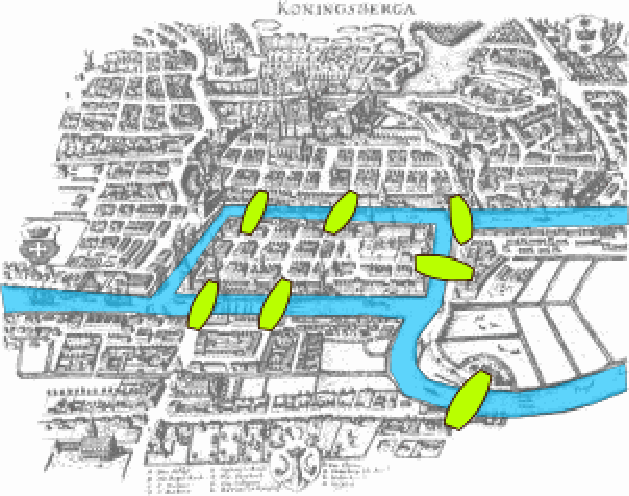
\includegraphics[width=0.5\textwidth]{images/bridges.pdf}
\caption{Mapa przedstawiająca mosty królewieckie za życia Leonharda Eulera. Źródło: \cite{wiki_mosty}}
\label{rys_mosty}
\end{figure}

\begin{de}
\textit{Grafem nieskierowanym} (\textit{niezorientowanym}) $G$ nazywamy parę $(V, E)$ składającą się z niepustego i skończonego zbioru \textit{wierzchołków} $V$ oraz skończonego zbioru krawędzi $E$
$$
E = \big\{ \{v_{i}, v_{j}\}\colon v_i, v_j\in V\big\}.
$$
\textit{Krawędzią} w grafie nieskierowanym o wierzchołkach $u, v\in V$ nazywamy dwuelementowy  zbiór $\{u, v\} \in E$ i mówimy, że krawędź $\{u, v\}$ jest \textit{incydentna} do wierzchołków $u$ i $v$. Do oznaczenia krawędzi grafu $\{u,v\}$ będziemy stosować notację $(u,v)$ - w tym przypadku zapis $(u,v)$ i $(v,u)$ oznacza tą samą krawędź (zob. przykład na rysunku \ref{rys_graf_niesk}).
\end{de}

\begin{figure}[H]
\centering
\begin{tikzpicture}[auto,node distance=1.5cm,semithick, every loop/.style={}]
    \node[main node] (1) {$1$};
    \node[main node] (2) [above left = 1.5cm and 0.2cm of 1]  {$2$};
    \node[main node] (3) [above right = 0.8cm and 1cm of 1] {$3$};
    \node[main node] (4) [right = of 3] {$4$};

    \path[draw,thick]
    (1) edge node {} (2)
    (1) edge node {} (3)
    (2) edge node {} (3)
    (3) edge node {} (4)
    (4) edge [in = 50, out = 100, loop] node {} (4);
\end{tikzpicture}
\caption{Graf nieskierowany $G =(V,E)$, gdzie $V = \{1,2,3,4\}$ i~$E = \big\{(1,2),(1,3),(2,3),(3,4),(4,4)\big\}$. Krawędź $(4,4)$ jest pętlą własną}
\label{rys_graf_niesk}
\end{figure}

\begin{de}
\textit{Grafem skierowanym} (\textit{zorientowanym} lub \textit{digrafem} z ang. \textit{directed graph}) $G$ nazywamy parę $(V, E)$, gdzie $E$ to zbiór krawędzi, a $V$ to zbiór wierzchołków. W przypadku grafu skierowanego zbiór krawędzi definiujemy jako zbiór uporządkowanych par:
$$
E = \big\{ (v_{i}, v_{j})\colon v_i, v_j\in V\big\}.
$$
Krawędź grafu skierowanego nazywana jest też \textit{łukiem}. Mówimy, że krawędź~$e=(u,v)\in E$ jest \textit{wychodząca} z wierzchołka $u$ i \textit{wchodząca} do wierzchołka $v$. (zob. przykład na rysunku \ref{rys_graf_sk}).
\end{de}

\begin{figure}[!htp]
\centering
\begin{tikzpicture}[->,>=stealth',auto,node distance=2cm,semithick]
    \node[main node] (1) {$1$};
    \node[main node] (2) [right = 4cm of 1]  {$2$};
    \node[main node] (3) [below = of 1] {$3$};
    \node[main node] (4) [right = of 3] {$4$};

    \path[draw,thick]
    (1) edge node {} (2)
    (1) edge node {} (4)
    (1)	edge node {} (3)
    (2) edge node {} (4)
    	edge [loop below] node {} (2)
    (3) edge [bend right] node {} (4)
    (4) edge [bend right] node {} (3);
\end{tikzpicture}

\caption{
Graf skierowany $G =(V,E)$, gdzie $V = \{1,2,3,4\}$ i $E = \big\{(1,2),(1,3),(1,4),(2,2),(2,4),(3,4),(4,3))\big\}$. Krawędź $(2,2)$ jest pętlą własną, krawędzie $(3,4)$ i $(4,3)$ są różne.}
\label{rys_graf_sk}
\end{figure}

\begin{de}
W grafie $G=(V,E)$, krawędź $e = (u,v)\in E$, dla której $u=v$ nazywamy \textit{pętlą własną}. 
Powtarzające się krawędzie lub pętle grafu $G$ (tzn. gdy $E$ jest \textit{multizbiorem}\footnote{Multizbiór jest uogólnieniem pojęcia zbioru, w którym jeden element (w naszym wypadku krawędź grafu) może występować więcej niż jeden raz.}) nazywamy \textit{równoległymi} lub \textit{wielokrotnymi}. Graf bez krawędzi wielokrotnych i pętli nazywamy \textit{grafem prostym}. Graf, który zawiera krawędzie lub pętle wielokrotne nazywamy \textit{multigrafem} (zob. przykład na rysunku \ref{rys_multigraf}).
\end{de}

\begin{figure}[!htp]
\centering
\begin{tikzpicture}[->,>=stealth',auto,node distance=2.8cm,semithick]
    \node[main node] (1) {$1$};
    \node[main node] (2) [above right = 4cm and 2 cm of 1]  {$2$};
    \node[main node] (3) [right = 4cm of 1] {$3$};

    \path[draw,thick]
    (1) edge node {} (2)
    (3) edge [bend left] node {} (1)
    	edge [bend right] node {} (1)
    (2) edge node {} (3)
    	edge [in=60, out=90, loop] node {} (2)
    (2)	edge [in=30, out=120, loop] node {} (2)
    	edge [bend left] node {} (3)
    	edge [bend right] node {} (3);
    	
%    \path[draw,thick] (2) edge [in=-10,out=120,loop] node[auto] {} (2);
\end{tikzpicture}
\caption{
Multigraf (skierowany) $G =(V,E)$, gdzie $V = \{1,2,3\}$ i~$E = \big\{(1,2),(2,2),(2,2),(2,3),(2,3),(2,3),(3,1),(3,1))\big\}$. Przedstawiony multigraf  zawiera między innymi trzy krawędzie $(2,3)$, które są równoległe. W tym przypadku nie da się odróżnić tych krawędzi i należałoby nadać odpowiednie etykiety każdej krawędzi (mielibyśmy do czynienia tzw. \textit{grafem etykietowanym}).}
\label{rys_multigraf}
\end{figure}

\begin{de}
\textit{Drogą} (\textit{ścieżką}) o długości $k$ w grafie $G = (V,E)$ prowadzącą z wierzchołka $u$ do wierzchołka $u'$ nazywamy ciąg wierzchołków $(v_i)_{i=0}^{k}$ takich, że $u = v_0$, $u'= v_k$ i $(v_i, v_{i+1}) \in E$ dla $i = 0,1,2,\dots, k-1$. \textit{Droga prosta} to szczególny przypadek drogi, w której wszystkie wierzchołki są różne. \textit{Długość drogi} to ilość jej krawędzi (lub wierzchołków nie licząc startowego).  Jeżeli istnieje ścieżka $\p$ z wierzchołka $u$~ do wierzchołka $v$ to mówimy, że $v$ jest osiągalny z $u$, co zapisujemy symbolicznie $u\stackrel{\p}{\leadsto}v$, jeżeli $G$ jest grafem skierowanym.
\end{de}

\begin{de}
Jeżeli graf $G = (V,E)$ jest skierowany to drogę $\p = (v_i)_{i=0}^{k}$ nazywamy \textit{cyklem} jeżeli $v_0 = v_k$. Analogicznie, \textit{cyklem prostym} nazywamy cykl, w którym wszystkie wierzchołki są różne poza wierzchołkiem początkowym i końcowym. W~grafie nieskierowanym droga $\p = (v_i)_{i=0}^{k}$ tworzy \textit{cykl}, jeżeli $k>0$,  $v_0 = v_k$ oraz wszystkie krawędzie są na tej drodze różne. \textit{Graf acykliczny} to taki graf, który nie zawiera cykli. 
\end{de}

\begin{de}
\textit{Grafem spójnym} nazywamy graf, w którym dla każdego wierzchołka $v \in V$ istnieje droga do każdego innego wierzchołka $v' \in V$. W takim przypadku graf nieskierowany nazywamy krótko \textit{grafem spójnym}, natomiast graf skierowany nazywamy \textit{grafem silnie spójnym}.
\end{de}
 
\begin{de}
\textit{Stopień wierzchołka} w grafie nieskierowanym to suma krawędzi incydentnych do niego. W grafie skierowanym dla każdego wierzchołka wyróżniamy \textit{stopień wejściowy} będący liczbą krawędzi do niego wchodzących oraz \textit{stopień wyjściowy}, który jest liczbą krawędzi z niego wychodzących. \textit{Stopniem wierzchołka} w grafie skierowanym nazywamy sumę stopni wchodzących i wychodzących. Pętle zwiększają stopień wierzchołka o $2$. Wierzchołek stopnia $0$ jest nazywany \textit{wierzchołkiem izolowanym}, a wierzchołek stopnia $1$ \textit{wierzchołkiem końcowym} albo \textit{wierzchołkiem wiszącym}.
\end{de}

\begin{de}
Gęstością grafu $G= (E,V)$ nazywamy stosunek liczby jego krawędzi do maksymalnej możliwej ilości krawędzi w grafie. W grafach prostych będą to więc odpowiednio liczby\footnote{Dla grafów prostych maksymalna ilość krawędzi w grafie skierowanym wynosi $|V|\big(|V|-1\big)$ natomiast w grafie nieskierowanym jest to $|V|\big(|V|-1\big)/2$.} 
\begin{itemize}
\item dla grafów nieskierowanych
$$
\rho(G) = \frac{2|E|}{|V|\big(|V|-1\big)}
$$
\item dla grafów skierowanych:
$$
\rho(G) = \frac{|E|}{|V|\big(|V|-1\big)}
$$
\end{itemize}

\textit{Grafem rzadkim} będziemy określić graf, w którym ilość wszystkich krawędzi $|E|$ jest dużo mniejsza niż kwadrat ilości wierzchołków $|V|^2$. Natomiast gdy ilość krawędzi będzie bliska $|V|^2$ to mówimy, że graf jest \textit{gęsty}\footnote{Jak można wywnioskować z tej definicji, pojęcie grafu rzadkiego i gęstego nie jest precyzyjne. Korzystając z pojęcia gęstości grafu możemy określać, dla jakiej wartości progowej graf uznajemy za rzadki lub gęsty.}.
\end{de}

\begin{de}
\textit{Drzewem} nazywamy nieskierowany graf, który jest acykliczny i spójny (zobacz rysunek \ref{rys_drzewo}). 
Wierzchołek drzewa o stopniu równym $1$ nazywamy \textit{liściem}. Drzewo, w którym jest wyróżniony jeden z wierzchołków nazywamy \textit{drzewem ukorzenionym}, a wyróżniony wierzchołek – \textit{korzeniem}. Graf nieskierowany i acykliczny, ale niekoniecznie spójny nazywamy \textit{lasem}.
\end{de}

\begin{figure}[H]
\centering
\begin{tikzpicture}[auto,node distance=1.5cm,semithick]
    \node[main node] (4) {$4$};
    \node[main node] (1) [above left = of 4]  {$1$};
    \node[main node] (2) [above = of 4] {$2$};
    \node[main node] (3) [above right = of 4] {$3$};
    \node[main node] (5) [below right = 1cm and 0.5cm of 4] {$5$};
    \node[main node] (6) [below left = 1cm of 5] {$6$};

    \path[draw,thick]
    (1) edge node {} (4)
    (2) edge node {} (4)
    (3) edge node {} (4)
    (4) edge node {} (4)
    (4) edge node {} (5)
    (5) edge node {} (6);
\end{tikzpicture}
\caption{Przykład grafu będącego drzewem.}
\label{rys_drzewo}
\end{figure}

\begin{de}
\textit{Grafem z wagami} lub \textit{grafem ważonym} nazywamy taki graf $G=(V, E)$, w którym z każdą krawędzią związana jest pewna liczba rzeczywista zwana \textit{wagą} lub \textit{kosztem}. Wagi krawędzi przeważnie określone są poprzez \textit{funkcję wagową} $w\colon E\to \bR$. Możemy zatem powiedzieć, że grafem ważonym nazywamy trójkę $G = (V, E, w)$, gdzie $w$ jest pewną funkcją wagową (zob. przykład na rysunku \ref{rys_graf_wa}). Jeżeli nie będzie to prowadzić do nieporozumień to w celu oznaczenia wartości funkcji wagowej (czyli wagi) dla $(u,v)\in E$ będziemy pisać $w(u,v)$ zamiast $w\big((u,v)\big)$.
\end{de}

\begin{figure}[H]
\centering
\begin{tikzpicture}[auto,node distance=2.8cm,semithick]
	\node[main node] (a) {$a$};
    \node[main node] (b) [below = 1cm of a]  {$b$};
    \node[main node] (c) [below = 1cm of b] {$c$};
    \node[main node] (d) [right = of c] {$d$};
    \node[main node] (e) [right = of d] {$e$};
    \node[main node] (f) [above = of e] {$f$};
    \node[main node] (g) [left = of f] {$g$};

    \path[draw,thick]
    (a) edge node {$5$} (b)
    (a) edge node {$6$} (g)
    (g) edge node {$-3$} (f)
    (g) edge node {$1$} (d)
    (g) edge node {$-8.5$} (b)
    (f) edge node {$11$} (e)
    (f) edge node {$3$} (d)
    (e) edge node {$-1$} (d)
    (d) edge node {$2$} (c)
    (d) edge node {$9$} (b)
    (c) edge node {$0.5$} (b);
\end{tikzpicture}
\caption{Przykład nieskierowanego grafu ważonego.}
\label{rys_graf_wa}
\end{figure}

\begin{de}
\textit{Graf dwudzielny} to taki graf, który można podzielić na dwa oddzielne zbiory wierzchołków, które nie będą połączone ze sobą wewnątrz tego zbioru. Można też stworzyć graf $K$-dzielny, zasada jest podobna, podział na $K$ rozłącznych zbiorów wierzchołków (zob. przykład na rysunku \ref{rys_graf_dwudzielny}).
\end{de}

\begin{figure}[!htp]
\centering
\begin{tikzpicture}[thick,
  every node/.style={draw,circle},
  fsnode/.style={fill=myblue,circle,fill=blue!20,draw,minimum size=1cm,inner sep=0pt},
  ssnode/.style={fill=mygreen,circle,fill=blue!20,draw,minimum size=1cm,inner sep=0pt},
  every fit/.style={ellipse,draw,inner sep=-2pt,text width=2cm}]

\begin{scope}[start chain=going below,node distance=7mm]
\foreach \i in {1,2}
  \node[fsnode,on chain] (f\i) {$\i$};
\end{scope}

\begin{scope}[xshift=4cm,start chain=going below,node distance=7mm]
\foreach \i in {3,4,5}
  \node[ssnode,on chain] (s\i) {$\i$};
\end{scope}

\node [myblue,fit=(f1) (f2)] {};
\node [mygreen,fit=(s3) (s5)] {};

\draw (f1) -- (s3);
\draw (s3) -- (f2);
\draw (f2) -- (s4);
\draw (s4) -- (f1);
\draw (f1) -- (s5);
\end{tikzpicture}
\caption{Przykład grafu dwudzielnego.
Jak widać podany graf dwudzielny można podzielić na $2$ zbiory wierzchołków $\{1,2\}$ oraz $\{3,4,5\}$.}
\label{rys_graf_dwudzielny}
\end{figure}

\begin{de}
Niech $G = (V, E, w)$ będzie grafem ważonym z funkcją wagową  $w\colon E\to \bR$. \textit{Wagą drogi} (\textit{długością drogi}) $\p = (v_i)_{i=0}^{k}$ nazywamy liczbę będącą sumą wag krawędzi tworzących tę drogę:
$$
w(\p) = \sum_{j = 0}^{k-1}w(v_{i}, v_{i+1}).
$$
Cykl o wadze ujemnej nazywamy \textit{cyklem ujemnym} (zob. przykład na rysunku \ref{rys_ujemny_cykl}).

\noindent
\textit{Wagę najkrótszej ścieżki} $\delta(u, v)$ z wierzchołka $u$ do wierzchołka $v$ definiujemy następująco:
$$
\delta(u, v) = 
\left\{
\begin{array}{ll}
\min\{w(\p)\colon\; u\stackrel{\p}{\leadsto}v\},&\quad \mbox{gdy istnieje droga z $u$ do $v$}\\
\infty, & \quad \mbox{gdy nie istnieje droga z $u$ do $v$}
\end{array}
\right..
$$
Każdą ścieżkę $\p$ z wierzchołka $u$ do wierzchołka $v$, dla której zachodzi równość $w(\p) =\delta(u, v)$ nazywamy \textit{najkrótszą ścieżką}.
\end{de}

\begin{figure}[H]
\centering
\begin{tikzpicture}[->,>=stealth',auto,node distance=2cm,semithick]
    \node[main node] (1) {$1$};
    \node[main node] (2) [above right = of 1]  {$2$};
    \node[main node] (4) [right = of 2] {$4$};
    \node[main node] (3) [below right = of 4] {$3$};

    \path[draw,thick]
    (1) edge node {$1$} (2)
    (1) edge node {$3$} (3)
    (2)	edge node {$-1$} (4)
    (4) edge [bend left] node {$2$} (3)
    (3) edge [bend left] node {$-6$} (4);
\end{tikzpicture}
\caption{Przykład skierowanego grafu ważonego zawierającego cykl ujemny.
Na podanym grafie pomiędzy wierzchołkiem $3$ oraz $4$ występuje ujemny cykl o wadze równej $-4$.}
\label{rys_ujemny_cykl}
\end{figure}

Analizując algorytmy będziemy często używać oznaczeń zaczerpniętych z teorii zbiorów: $|V|$ i $|E|$ dla oznaczenia odpowiednio liczby wszystkich wierzchołków grafu oraz liczby wszystkich krawędzi w grafie\footnote{Chodzi tu konkretnie o symbole oznaczające \textit{moc zbioru}, czyli liczbę jego elementów.}. Często też, ilość wierzchołków w grafie $G$ będziemy oznaczać symbolem $n$, a liczbę krawędzi symbolem $m$. Dodatkowo podczas analizy złożoności algorytmów zazwyczaj podaje się sam symbol bez dodatkowych znaków, na przykład $V^2$ zamiast $|V|^2$.

Istnieje wiele rodzajów grafów, ale najprostszym podziałem będzie podział na:
\begin{itemize}
\item Grafy nieskierowane (\textit{niezorientowane})
\item Grafy skierowane (\textit{zorientowane})
\item Grafy ważone
\item Drzewa
\item Multigrafy
\end{itemize}

\section{Reprezentacja grafów w komputerze}

Istnieją dwa najpopularniejsze sposoby reprezentacji grafów w pamięci komputera:
\begin{itemize}
\item Lista sąsiedztwa
\item Macierz sąsiedztwa
\end{itemize}

\textit{Lista sąsiedztwa} to taka struktura danych, w której dla każdego wierzchołka w~grafie tworzymy listę sąsiadujących z nim wierzchołków.

\begin{figure}[H]
\centering
\begin{tabular}{l}
	\vspace{0.4em}
	1 \begin{tabular}{| c |} \hline	$\cdot$\\ \hline \end{tabular}
	$\rightarrow$
	\begin{tabular}{| c | c |} \hline 2 & $\cdot$\\ \hline \end{tabular}
	$\rightarrow$
	\begin{tabular}{| c | c |} \hline 3 & /\\ \hline \end{tabular} \\
	\vspace{0.4em}
	2 \begin{tabular}{| c |} \hline $\cdot$\\ \hline \end{tabular}
	$\rightarrow$
	\begin{tabular}{| c | c |} \hline 1 & $\cdot$\\ \hline \end{tabular}
	$\rightarrow$
	\begin{tabular}{| c | c |} \hline 3 & /\\ \hline \end{tabular} \\
	\vspace{0.4em}
	3 \begin{tabular}{| c |} \hline	$\cdot$\\ \hline \end{tabular}
	$\rightarrow$
	\begin{tabular}{| c | c |} \hline 1 & $\cdot$\\ \hline \end{tabular}
	$\rightarrow$
	\begin{tabular}{| c | c |} \hline 2 & $\cdot$\\ \hline \end{tabular}
	$\rightarrow$
	\begin{tabular}{| c | c |} \hline 4 & /\\ \hline \end{tabular} \\
	\vspace{0.4em}
	4 \begin{tabular}{| c |} \hline $\cdot$\\ \hline \end{tabular}
	$\rightarrow$
	\begin{tabular}{| c | c |} \hline 3 & $\cdot$\\ \hline \end{tabular}
	$\rightarrow$
	\begin{tabular}{| c | c |} \hline 4 & /\\ \hline \end{tabular} \\
\end{tabular}
\caption{Lista sąsiedztwa grafu nieskierowanego z rysunku \ref{rys_graf_niesk}.}
\label{rys_lista_sasiedztwa_nieskierowany}
\end{figure}

\begin{figure}[H]
\centering
\begin{tabular}{l}
	\vspace{0.4em}
	1 \begin{tabular}{| c |} \hline /\\ \hline \end{tabular} \\
	\vspace{0.4em}
	2 \begin{tabular}{| c |} \hline	$\cdot$\\ \hline \end{tabular}
	$\rightarrow$
	\begin{tabular}{| c | c |} \hline 1 & /\\ \hline \end{tabular} \\
	\vspace{0.4em}
	3 \begin{tabular}{| c |} \hline	$\cdot$\\ \hline \end{tabular}
	$\rightarrow$
	\begin{tabular}{| c | c |} \hline 2 & $\cdot$\\ \hline \end{tabular}
	$\rightarrow$
	\begin{tabular}{| c | c |} \hline 5 & /\\ \hline \end{tabular} \\
	\vspace{0.4em}
	4 \begin{tabular}{| c |} \hline	$\cdot$\\ \hline \end{tabular}
	$\rightarrow$
	\begin{tabular}{| c | c |} \hline 2 & /\\ \hline \end{tabular} \\
	\vspace{0.4em}
	5 \begin{tabular}{| c |} \hline	$\cdot$\\ \hline \end{tabular}
	$\rightarrow$
	\begin{tabular}{| c | c |} \hline 3 & $\cdot$\\ \hline \end{tabular}
	$\rightarrow$
	\begin{tabular}{| c | c |} \hline 4 & /\\ \hline \end{tabular} \\
	\vspace{0.4em}
	6 \begin{tabular}{| c |} \hline	$\cdot$\\ \hline \end{tabular}
	$\rightarrow$
	\begin{tabular}{| c | c |} \hline 3 & /\\ \hline \end{tabular} \\
\end{tabular}
\caption{Lista sąsiedztwa przykładowego grafu skierowanego przedstawionego na rysunku \ref{rys_DiGraf}.}
\label{rys_lista_sasiedztwa_skierowany}
\end{figure}

\begin{figure}[H]
\centering
\begin{tikzpicture}[->,>=stealth',auto,node distance=2cm,semithick]
    \node[main node] (1) {$1$};
    \node[main node] (2) [right = of 1]  {$2$};
    \node[main node] (3) [below right = of 2] {$3$};
    \node[main node] (4) [below = of 2] {$4$};
    \node[main node] (5) [below right = of 4] {$5$};
    \node[main node] (6) [above right = of 3] {$6$};

    \path[draw,thick]
    (2) edge node {} (1)
    (4) edge node {} (2)
    (3)	edge node {} (2)
    (5) edge node {} (4)
    (5) edge [bend left] node {} (3)
    (3) edge [bend left] node {} (5)
    (6) edge node {} (3);
\end{tikzpicture}
\caption{Przykładowy graf skierowany.}
\label{rys_DiGraf}
\end{figure}

W celu zaimplementowania listy sąsiedztwa w języku Python musimy stworzyć listę wierzchołków, a każdy wierzchołek będzie listą sąsiednich wierzchołków więc otrzymujemy listę list. W przypadku grafu ważonego, listę zastępujemy słownikiem, aby dodatkowo opisać wagi na krawędziach. Najprostszy przykład kodu w języku Python dla grafu przedstawionego na rysunku \ref{rys_graf_niesk} może obrazować kod źródłowy z~rysunku \ref{Python_lista_sasiedztwa_nieskierowany}. Bardziej złożony graf skierowany z rysunku \ref{rys_DiGraf} może być zaimplementowany w Pythonie jak na rysunku \ref{Python_lista_sasiedztwa_skierowany}.

\lstinputlisting[label = Python_lista_sasiedztwa_nieskierowany, caption = {Kod \'{z}r\'{o}d\l{}owy implementacji listy s\k{a}siedztwa grafu nieskierowanego.}]{python_source/lista_sasiedztwa_nieskierowany.py}


\lstinputlisting[label = Python_lista_sasiedztwa_skierowany, caption = {Kod \'{z}r\'{o}d\l{}owy implementacji listy s\k{a}siedztwa grafu skierowanego.}]{python_source/lista_sasiedztwa_skierowany.py}

\textit{Macierz sąsiedztwa} to macierz kwadratowa $\bb A = [a_{ij}]$ o rozmiarze $n \times n$ ($n$ to liczba wierzchołków grafu) taka, że $a_{ij} = 1$, jeżeli w grafie istnieje krawędź $(i,j)$, a~$a_{ij} = 0$, jeżeli nie istnieje. Jeśli graf jest nieskierowany to macierz sąsiedztwa jest symetryczna. 

\begin{figure}[H]
$$
\bb A = 
\begin{bmatrix}
0 & 0 & 0 & 0 & 0 & 0\\
1 & 0 & 0 & 0 & 0 & 0\\
0 & 0 & 1 & 0 & 1 & 0\\
0 & 0 & 1 & 0 & 0 & 0\\
0 & 0 & 1 & 1 & 0 & 0\\
0 & 0 & 1 & 0 & 0 & 0\\
\end{bmatrix}
$$
\caption{Macierz sąsiedztwa dla grafu z rysunku \ref{rys_DiGraf}}
\label{macierz}
\end{figure}

Aby zaimplementować macierz sąsiedztwa w języku Python należy stworzyć listę list $n$ - wymiarowych, gdzie $n$ to liczba wierzchołków w grafie, dla grafu z rysunku \ref{rys_DiGraf} macierz sąsiedztwa przedstawia rysunek \ref{Python_macierz_sasiedztwa}

\lstinputlisting[label = Python_macierz_sasiedztwa, caption = {Kod \'{z}r\'{o}d\l{}owy implementacji macierzy s\k{a}siedztwa.}]{python_source/macierz_sasiedztwa.py}

\section{Podstawowe algorytmy badania grafów}
\textit{Badanie grafu} to algorytmiczne przejście każdego wierzchołka grafu i sprawdzenie (zbadanie) relacji z innymi wierzchołkami. Można dzięki temu znajdować m.in.: \textit{spójne składowe grafu}, ścieżki między wierzchołkami (w tym dla grafów nieważonych te najkrótsze) lub badać czy dany graf jest dwudzielny.

Najprostszymi algorytmami badającymi grafy są 2 podstawowe algorytmy:
\begin{itemize}
\item Przeszukiwania wszerz (\textit{BFS})
\item Przeszukiwania wgłąb (\textit{DFS})
\end{itemize}

Są one używane w wielu bardziej skomplikowanych algorytmach. Przykładem użycia przeszukiwania w głąb jest \textit{sortowanie topologiczne} \textit{skierowanych grafów acyklicznych} (z ang. \textit{directed acyclic graph}, w skrócie \textit{DAG}), polegające na uporządkowaniu w porządku liniowym wierzchołków w taki sposób, aby każdy kolejny wierzchołek wymagał poprzedniego, czyli relacja między dwoma wierzchołkami przechodziła od poprzedniego do następnego. Popularnym zastosowaniem DAG-ów jest analiza sieci PERT\footnote{\textit{PERT} (z ang. \textit{Program Evaluation and Review Technique}) - metoda planowania i zarządzania projektem, przedstawiana jako graf skierowany z wagami, którego wierzchołki stanowią zadania realizowane w ramach projektu oraz krawędzie z wagami mówiące o czasie potrzebnym na wykonanie zadania.}. 

\section{Problem najkrótszych ścieżek w grafie ważonym}

Problem znajdowania najkrótszej ścieżki między dwoma wierzchołkami $u$ i $v$ w~grafie ważonym sprowadza się do wyznaczenia drogi, która prowadzi z wierzchołka $u$~do $v$, której waga (koszt) jest minimalna. Istnieją różne odmiany algorytmów wyznaczania najkrótszych ścieżek w grafach:
\begin{itemize}
\item \textbf{Najkrótsze ścieżki z jednym wierzchołkiem źródłowym.} W problemie tym wyróżniamy jeden wierzchołek $s$ (zwany \textit{źródłem}, ang. \textit{source}) grafu $G$ i poszukujemy najkrótszych ścieżek z wierzchołka $s$ do pozostałych wierzchołków grafu.
\item \textbf{Najkrótsze ścieżki z jednym wierzchołkiem docelowym.} Wyróżniamy w grafie $G$ jeden wierzchołek docelowy $t$ (ang. \textit{target}) i poszukujemy najkrótszy ścieżek ze wszystkich pozostałych wierzchołków grafu $G$ do wierzchołka $t$. Łatwo zauważyć, że gdy zmienimy zwroty wszystkich krawędzi (w grafach skierowanych) na przeciwne to problem ten sprowadza się do wyznaczenia najkrótszych ścieżek z jednym wierzchołkiem źródłowym.
\item \textbf{Najkrótsze ścieżki między parą wierzchołków.} W tym problemie poszukujemy najkrótszej drogi prowadzącej z pewnego wierzchołka $u$ do innego wierzchołka $v$. Niestety okazuje się, że w pesymistycznym przypadku żaden algorytm rozwiązujący ten problem nie jest szybszy od algorytmu rozwiązującego problem najkrótszych ścieżek z jednym źródłem.
\item \textbf{Najkrótsze ścieżki między wszystkimi parami wierzchołków.} Poszukujemy najkrótszych ścieżek między wszystkimi parami wierzchołków danego grafu $G$.

\end{itemize}

Dla problemu z jednym wierzchołkiem źródłowym lub docelowym użyć można algorytmu \textit{Djikstry}, wymaga on, by w całym grafie nie było krawędzi o ujemnych wagach.
Bardziej ogólnym algorytmem dla problemu z jednym źródłem, w którym dopuszczamy występowanie wag ujemnych jest algorytm \textit{Bellmana-Forda}. 
Dla problemu najkrótszych ścieżek między wszystkimi parami wierzchołków można oczywiście użyć algorytmu Djikstry lub Bellmana-Forda (kolejno traktując jako źródło wszystkie wierzchołki grafu). Rozwiązanie to jest jednak bardzo nieefektywne. Na szczęście istnieją lepsze algorytmy dla problemu wyznaczenia najkrótszych ścieżek między wszystkimi parami wierzchołków m.in. algorytm \textit{Floyda-Warshalla} oraz algorytm \textit{Johnsona} (efektywny dla grafów rzadkich).



%############################################################################################
%############################################################################################
%-----------       Rozdział 2. Omówienie wybranych algorytmów          -----------# %############################################################################################
%############################################################################################

\chapter{Omówienie wybranych algorytmów}\label{ch_2}

W tym rozdziale zostaną dokładnie przedstawione wspominane już algorytmy wyznaczania najkrótszych ścieżek w grafach ważonych. W szczególności podamy pseudokody tych algorytmów, które podobnie jak podane tu informacje można znaleźć m.in. w~\cite{ALG_BEZ_TAJ, CORMEN}.

\section{Algorytmy wyznaczające ścieżki z jednego źródła}

Na początek opiszemy algorytmy  Dijkstry oraz Bellmana-Forda, które rozwiązują problem wyznaczania najkrótszej drogi w grafie z jednym wierzchołkiem źródłowym.

\subsection{Algorytm Dijkstry}

Algorytm Dijkstry przeznaczony jest do znajdowania najkrótszych ścieżek w~skierowanych grafach ważonych o wagach nieujemnych. Zakładamy więc, że mamy graf ważony $G = (V, E)$ z funkcją wagową $w$ taką, że $w(u, v) \geq 0$ dla każdej krawędzi $(u,v)\in E$. Poza tym w zbiorze wierzchołków $V$ grafu $G$ wyróżniamy wierzchołek źródłowy $s$. Algorytm wyznacza w grafie wszystkie najkrótsze ścieżki między wierzchołkiem źródłowym, a pozostałymi wierzchołkami grafu oraz wyznacza koszt przejścia każdej z tych ścieżek.

W algorytmie Dijkstry z każdym wierzchołkiem $v\in V$ grafu $G$ wiążemy dwie wartości. Pierwszą z nich jest $d[v]$, która jest aktualnym górnym oszacowaniem kosztu najkrótszej drogi z wierzchołka źródłowego do wierzchołka $v$. Drugą wartością jest $p[v]$, która zawiera poprzedni wierzchołek (tzw. poprzednik) do $v$ na chwilowo najkrótszej drodze ze źródła do $v$. Ponadto, w omawianym algorytmie wykorzystuje się tzw. operację \textit{relaksacji} (inaczej \textit{osłabiania ograniczeń}).

\begin{de}
Relaksacją krawędzi $(u, v)$ grafu $G$ przy uwzględnieniu wierzchołka źródłowego $s$ nazywamy proces polegający na sprawdzeniu, czy przechodząc przez wierzchołek $u$ można wyznaczyć krótszą ścieżkę (tj. o mniejszym koszcie) między $v$~i~$s$ od dotychczas wyznaczonej. Jeżeli w wyniku tego sprawdzania taka możliwość istnieje to następuje odpowiednia aktualizacja wartości $d[v]$ i $p[v]$. W wyniku relaksacji może uleć zmienieniu wartość oszacowania kosztu najkrótszej drogi $d[v]$ i może uleć zmianie poprzednik $p[v]$ (zobacz rysunek \ref{RELAX_pseudokod}).

\begin{figure}[ht]
\begin{myalgorithm}[H]
	\DontPrintSemicolon
	\SetKwFunction{FMain}{relax}
	\SetKwProg{Fn}{Function}{:}{}
	\Fn{\FMain{$u$, $v$, $w$}}{
	\If{$d[v] \ge d[u] + w(u, v)$}
		{
		$d[v] = d[u] + w(u, v)$\;
		$p[v] = u $\;
		}
	}
\end{myalgorithm}
\caption{Pseudokod procedury relaksacji.}
\label{RELAX_pseudokod}
\end{figure}
\end{de}

W prezentowanym algorytmie Dijkstry (rysunek \ref{Dijkstra_pseudokod}) przyjmuje się początkowo, dla każdego wierzchołka $v\in V$, że $d[v]$ = $\infty$ oraz $d[s]$ = 0. Ponadto, dla każdego wierzchołka $v \in V$ przyjmujemy początkowo $p[v]$ = $\mbox{Null}$, co oznacza brak poprzednika \footnote{W zależności od implementacji może to być wartość $0$, $\mbox{Null}$ lub $\mbox{None}$.}. W trakcie działania algorytmu pamiętany jest (początkowo pusty) zbiór $S$, w którym umieszczane są wierzchołki, dla których koszt najkrótszej drogi ze źródła $s$~został już obliczony. Używana jest także  kolejka priorytetowa (typu min) $Q = V/S$, w której znajdą się wierzchołki jeszcze nieprzetworzone (wierzchołki są zorganizowane według wartości $d$).  Następnie algorytm wykonuje wielokrotnie następujące kroki: 
\begin{itemize}
\item wybiera z kolejki $Q$ wierzchołek $u$ o najmniejszej wartości oszacowania $d[u]$ i~usuwa go z niej (operacja $\texttt{extract\_min}$);
\item dodaje wierzchołek $u$ do zbioru $S$;
\item wykonuje relaksację dla wszystkich krawędzi wychodzących z wierzchołka $u$.
\end{itemize}

\begin{figure}[ht]
\begin{myalgorithm}[H]
	\DontPrintSemicolon
	\SetKwFunction{FMain}{dijkstra}
	\SetKwProg{Fn}{Function}{:}{}
	\Fn{\FMain{$G$, $w$, $s$}}{
		\ForAll{$v \in V(G)$}
		{
			$d[v] = \infty $\;
			$p[v] = \mbox{Null} $\;		
		}
		$d[s] = 0$\;
		$S = \emptyset $\;
		$Q = V(G)$\;
		\While{$Q \neq \emptyset $}
		{
			$u = \mbox{extract\_min}(Q)$\;
			$S = S \cup \{u\}$\;
			\ForAll{$v \in Adj[u]$}
			{
				$\mbox{relax}(u, v, w)$\;			
			}
		}
	}
\end{myalgorithm}
\caption{Pseudokod algorytmu Dijkstry.}
\label{Dijkstra_pseudokod}
\end{figure}

W wyniku działania algorytmu Dijkstry dla każdego wierzchołka $v$ otrzymujemy wartości $d[v]$, która jest najmniejszym kosztem drogi z wierzchołka $s$ do wierzchołka $v$ (tj. wagą najkrótszej ścieżki z $s$ do $v$).  Z kolei, dzięki wartości $p[v]$ możemy odczytać drogę o koszcie $d[v]$, odczytując kolejno $v$, $p[v]$, $p[p[v]]$ itd. aż dojedziemy do $s$.

Warto zauważyć, że w algorytmie Dijskstry do zbioru $S$ za każdym razem dodawany jest wierzchołek $v \in V/S$ o aktualnie najmniejszej wartości $d[v]$. Jest to zatem przykład algorytmu zachłannego. Można wykazać, że wyniku działania tego algorytmu zawsze otrzymujemy optymalne rozwiązanie.

\begin{ex}
Przeanalizujmy działanie algorytmu Dijkstry (ryunek \ref{Dijkstra_pseudokod}) dla przykładowego grafu (rysunek \ref{rys_Dijkstra_przyklad}), gdzie jako wierzchołek źródłowy wybieramy wierzchołek $a$. Etapy działania algorytmu (iteracje drugiej pętli)  możemy zobaczyć na rysunku \ref{rys_przeb_alg_Dijkstry}. Kolejne ilustracje prezentują przetwarzanie kolejnych wierzchołków: $a$, $b$, $c$, $d$ oraz $f$.

\begin{figure}[!htp]
\centering
\begin{tikzpicture}[->, >=stealth', auto, node distance=2cm, semithick]
		\node[main node] (a) {$a$};
	    \node[main node] (b) [right = 1cm of a]  {$b$};
	    \node[main node] (c) [below = of a] {$c$};
	    \node[main node] (d) [right = of c] {$d$};
	    \node[main node] (e) [below left = of d] {$e$};
	    \node[main node] (f) [left = of c] {$f$};
	
	    \path[draw,thick]
	    (a) edge node {$7$} (b)
	    (a) edge node {$9$} (c)
	    (a) edge node {$14$} (f)
	    (b) edge node {$10$} (c)
	    (b) edge node {$15$} (d)
	    (c) edge node {$11$} (d)
	    (c) edge node {$2$} (f)
	    (d) edge node {$6$} (e)
	    (e) edge node {$9$} (f);
\end{tikzpicture}
\caption{Przykładowy graf ważony o wagach nieujemnych.}
\label{rys_Dijkstra_przyklad}
\end{figure}

\begin{figure}[!htp]
\centering
\begin{subfigure}[b]{0.4\textwidth}
	\begin{tikzpicture}[->, >=stealth', auto, node distance=1cm, semithick]
		\node[main node, fill=mygreen!60] (a) {$a/0$};
	    \node[main node] (b) [right = 1cm of a]  {$b/7$};
	    \node[main node] (c) [below = of a] {$c/9$};
	    \node[main node] (d) [right = of c] {$d/\infty$};
	    \node[main node] (e) [below left = of d] {$e/\infty$};
	    \node[main node] (f) [left = of c] {$f/14$};
	
	    \path[draw,thick]
	    (a) edge [red] node {$7$} (b)
	    (a) edge [red] node {$9$} (c)
	    (a) edge [red] node {$14$} (f)
	    (b) edge node {$10$} (c)
	    (b) edge node {$15$} (d)
	    (c) edge node {$11$} (d)
	    (c) edge node {$2$} (f)
	    (d) edge node {$6$} (e)
	    (e) edge node {$9$} (f);
	\end{tikzpicture}
	\caption{Przetwarzanie wierzchołka "a".}
	\label{rys_dijkstra_przyklad_1}
\end{subfigure}
~
\begin{subfigure}[b]{0.4\textwidth}
	\begin{tikzpicture}[->, >=stealth', auto, node distance=1cm,semithick]
		\node[main node, fill=mygreen!60] (a) {$a/0$};
	    \node[main node, fill=mygreen!60] (b) [right = 1cm of a]  {$b/7$};
	    \node[main node] (c) [below = of a] {$c/9$};
	    \node[main node] (d) [right = of c] {$d/22$};
	    \node[main node] (e) [below left = of d] {$e/\infty$};
	    \node[main node] (f) [left = of c] {$f/14$};
	
	    \path[draw,thick]
	    (a) edge [red] node {$7$} (b)
	    (a) edge [red] node {$9$} (c)
	    (a) edge [red] node {$14$} (f)
	    (b) edge node {$10$} (c)
	    (b) edge [red] node {$15$} (d)
	    (c) edge node {$11$} (d)
	    (c) edge node {$2$} (f)
	    (d) edge node {$6$} (e)
	    (e) edge node {$9$} (f);
	\end{tikzpicture}
	\caption{Przetwarzanie wierzchołka "b".}
	\label{rys_dijkstra_przyklad_2}
\end{subfigure}

\begin{subfigure}[b]{0.4\textwidth}
	\begin{tikzpicture}[->, >=stealth', auto, node distance=1cm, semithick]
		\node[main node, fill=mygreen!60] (a) {$a/0$};
	    \node[main node, fill=mygreen!60] (b) [right = 1cm of a]  {$b/7$};
	    \node[main node, fill=mygreen!60] (c) [below = of a] {$c/9$};
	    \node[main node] (d) [right = of c] {$d/20$};
	    \node[main node] (e) [below left = of d] {$e/\infty$};
	    \node[main node] (f) [left = of c] {$f/11$};
	
	    \path[draw,thick]
	    (a) edge [red] node {$7$} (b)
	    (a) edge [red] node {$9$} (c)
	    (a) edge node {$14$} (f)
	    (b) edge node {$10$} (c)
	    (b) edge node {$15$} (d)
	    (c) edge [red] node {$11$} (d)
	    (c) edge [red] node {$2$} (f)
	    (d) edge node {$6$} (e)
	    (e) edge node {$9$} (f);
	\end{tikzpicture}
	\caption{Przetwarzanie wierzchołka "c".}
	\label{rys_dijkstra_przyklad_3}
\end{subfigure}
~
\begin{subfigure}[b]{0.4\textwidth}
	\begin{tikzpicture}[->, >=stealth', auto, node distance=1cm,semithick]
		\node[main node, fill=mygreen!60] (a) {$a/0$};
	    \node[main node, fill=mygreen!60] (b) [right = 1cm of a]  {$b/7$};
	    \node[main node, fill=mygreen!60] (c) [below = of a] {$c/9$};
	    \node[main node, fill=mygreen!60] (d) [right = of c] {$d/20$};
	    \node[main node] (e) [below left = of d] {$e/\infty$};
	    \node[main node] (f) [left = of c] {$f/11$};
	
	    \path[draw,thick]
	    (a) edge [red] node {$7$} (b)
	    (a) edge [red] node {$9$} (c)
	    (a) edge node {$14$} (f)
	    (b) edge node {$10$} (c)
	    (b) edge node {$15$} (d)
	    (c) edge [red] node {$11$} (d)
	    (c) edge [red] node {$2$} (f)
	    (d) edge node {$6$} (e)
	    (e) edge node {$9$} (f);
	\end{tikzpicture}
	\caption{Przetwarzanie wierzchołka "d".}
	\label{rys_dijkstra_przyklad_4}
\end{subfigure}

\begin{subfigure}[b]{0.4\textwidth}
	\begin{tikzpicture}[->, >=stealth', auto, node distance=1cm, semithick]
		\node[main node, fill=mygreen!60] (a) {$a/0$};
	    \node[main node, fill=mygreen!60] (b) [right = 1cm of a]  {$b/7$};
	    \node[main node, fill=mygreen!60] (c) [below = of a] {$c/9$};
	    \node[main node, fill=mygreen!60] (d) [right = of c] {$d/20$};
	    \node[main node, fill=mygreen!60] (e) [below left = of d] {$e/26$};
	    \node[main node] (f) [left = of c] {$f/11$};
	
	    \path[draw,thick]
	    (a) edge [red] node {$7$} (b)
	    (a) edge [red] node {$9$} (c)
	    (a) edge node {$14$} (f)
	    (b) edge node {$10$} (c)
	    (b) edge node {$15$} (d)
	    (c) edge [red] node {$11$} (d)
	    (c) edge [red] node {$2$} (f)
	    (d) edge [red] node {$6$} (e)
	    (e) edge node {$9$} (f);
	\end{tikzpicture}
	\caption{Przetwarzanie wierzchołka "f".}
	\label{rys_dijkstra_przyklad_5}
\end{subfigure}
~
\begin{subfigure}[b]{0.4\textwidth}
	\begin{tikzpicture}[->, >=stealth', auto, node distance=1cm,semithick]
		\node[main node, fill=mygreen!60] (a) {$a/0$};
	    \node[main node, fill=mygreen!60] (b) [right = 1cm of a]  {$b/7$};
	    \node[main node, fill=mygreen!60] (c) [below = of a] {$c/9$};
	    \node[main node, fill=mygreen!60] (d) [right = of c] {$d/20$};
	    \node[main node, fill=mygreen!60] (e) [below left = of d] {$e/26$};
	    \node[main node, fill=mygreen!60] (f) [left = of c] {$f/11$};
	
	    \path[draw,thick]
	    (a) edge [red] node {$7$} (b)
	    (a) edge [red] node {$9$} (c)
	    (a) edge node {$14$} (f)
	    (b) edge node {$10$} (c)
	    (b) edge node {$15$} (d)
	    (c) edge [red] node {$11$} (d)
	    (c) edge [red] node {$2$} (f)
	    (d) edge [red] node {$6$} (e)
	    (e) edge node {$9$} (f);
	\end{tikzpicture}
	\caption{Przetwarzanie wierzchołka "e".}
	\label{rys_dijkstra_przyklad_6}
\end{subfigure}

\caption{Przebieg algorytmu Dijkstry dla grafu \ref{rys_Dijkstra_przyklad}}\label{rys_przeb_alg_Dijkstry}
\end{figure}

Wierzchołki zaznaczone na zielono to wierzchołki, które zostały już przetworzone (odwiedzone) przez algorytm. Kolorem czerwonym zaznaczamy krawędzie prowadzące od poprzednika do rozważanego wierzchołka, tworzymy z nich najkrótsze ścieżki, dla przykładu: jeżeli chcemy odczytać najkrótszą drogę od źródła ($a$) do wierzchołka $f$ należy popatrzeć na rysunek \ref{rys_dijkstra_przyklad_6}. Dla wierzchołka $f$ poprzednikiem jest wierzchołek $c$ więc krawędź $(c,f)$ jest zaznaczona na czerwono, dalej poprzednikiem $c$ jest $a$, wierzchołek $a$ nie ma już poprzedników (bo jest startowy). Otrzymujemy zatem najkrótszą drogę: $a \rightarrow c \rightarrow f$. Z gotowych poprzedników powstaje tzw. \textit{drzewo najkrótszych ścieżek} o korzeniu w wierzchołku źródłowym, jest to podgraf wejściowego grafu, który zawiera tylko krawędzie, z których można utworzyć najkrótsze ścieżki. 
\end{ex}

\subsection{Algorytm Bellmana-Forda}

Algorytm Bellmana-Forda jest uogólnioną wersją algorytmu Dijkstry. Podstawową wadą algorytmu Dijkstry jest niemożność zastosowania go do grafów z wagami ujemnymi. Wynika to z faktu, że korzysta on z założenia iż dodanie do ścieżki dodatkowej krawędzi może ją tylko wydłużyć - uwzględnienie wag ujemnych w naturalny sposób psuje to założenie. Algorytm Bellmana-Forda wyznacza najkrótsze ścieżki w gafie ważonym (również o wagach ujemnych) z ustalonego wierzchołka $s$ do pozostałych wierzchołków grafu. W przypadku wystąpienia w grafie cyklu ujemnego, algorytm Bellmana-Forda nie może wyznaczyć szukanej drogi\footnote{Oczywiście, w takiej sytuacji w grafie nie da się w ogóle wyznaczyć najkrótszych ścieżek.}, ale wykrywa taką sytuację - dlatego często jest używany do wykrywania cykli ujemnych w grafach ważonych. 

\begin{figure}[H]
\begin{myalgorithm}[H]
	\DontPrintSemicolon
	\SetKwFunction{FMain}{bellman-ford}
	\SetKwProg{Fn}{Function}{:}{}
	\Fn{\FMain{$G$, $w$, $s$}}
	{
		\ForAll{$v \in V(G)$}
		{
			$d[v] = \infty $\;
			$p[v] = \mbox{Null} $\;		
		}
		$d[s] = 0$\;
		\For{$i \leftarrow 1$ \KwTo $\big|V[G]\big| - 1$}
		{
			\ForAll{$(u, v) \in E(G)$}
			{
				$\mbox{relax}(u, v, w)$\;
			}
		}
		\ForAll{$(u, v) \in E(G)$}
		{
			\If{$d[v] > d[u] + w(u, v)$}
			{
				\Return $\mbox{False}$\;
			}
		}
		\Return $\mbox{True}$ \;
	}
\end{myalgorithm}
\caption{Pseudokod algorytmu Bellmana-Forda.}
\label{Bellman_Ford_pseudokod}
\end{figure}

W omawianym algorytmie również używana jest relaksacja, lecz zamiast wykonywać relaksację tylko na tych krawędziach, które zapewniają minimalizację wagi, relaksacja jest wykonywana dla wszystkich $n - 1$ krawędzi, gdzie $n$ to liczba wierzchołków w grafie. Następnie sprawdzane jest wystąpienie cyklu ujemnego w badanym grafie. Jeżeli odległość od końcowego wierzchołka jest mniejsza niż odległość od wierzchołka początkowego powiększona o wagę danej krawędzi to musiał wystąpić cykl o ujemnej wadze, zwracany jest wtedy błąd w postaci zmiennej logicznej \texttt{False}.

Zwracany wynik algorytmu Bellmana-Forda jest identyczny do wyniku algorytmu Dijkstry. W celu ilustracji działania algorytmu Bellmana-Forda przeanalizujemy dwa przykłady grafów - jeden z cyklem ujemnym, a drugi bez.

\begin{ex}
Rozważmy graf przedstawiony na rysunku \ref{rys_Bellman_Ford_ujemny_cykl} z cyklem o wadze ujemnej ($c \rightarrow d \rightarrow e \rightarrow c$) równej $-7$. Przeanalizujmy działanie algorytmy Bellmana-Forda dla tego grafu, gdy jako wierzchołek źródłowy wybierzemy $a$.

\begin{figure}[H]
\centering
\begin{tikzpicture}[->, >=stealth', auto, node distance=1.5cm, semithick]
		\node[main node, minimum size=1.4cm] (a) {$a$};
	    \node[main node, minimum size=1.4cm] (b) [below right = 1.5cm of a]  {$b$};
	    \node[main node, minimum size=1.4cm] (c) [left = of a] {$c$};
	    \node[main node, minimum size=1.4cm] (d) [below = of c] {$d$};
	    \node[main node, minimum size=1.4cm] (e) [right = of d] {$e$};
	
	    \path[draw,thick]
	    (a) edge [bend left] node {$3$} (b)
	    (b) edge [bend left] node {$2$} (a)
	    (a) edge node {$10$} (c)
	    (c) edge node {$-9$} (d)
	    (d) edge node {$7$} (e)
	    (e) edge node {$1$} (a)
	    (e) edge node {$-5$} (c);
\end{tikzpicture}
\caption{Przykładowy graf ważony zawierający ujemny cykl.}
\label{rys_Bellman_Ford_ujemny_cykl}
\end{figure}
Rysunek \ref{rys_bf_ujemny_cykl_przyklad_4} przedstawia wynik algorytmu. Żeby wynik był poprawny dla każdej krawędzi należy przeprowadzić sprawdzanie z 10 linii pseudokodu (\textbf{\texttt{if}} $d[v] > d[u] + w(u,v)$ \textbf{\texttt{then return}} \texttt{False}). W tym przypadku sprawdzanie to zakończy się zwróceniem wartości \texttt{False}.
\begin{figure}[H]
\centering
\begin{subfigure}[b]{0.4\textwidth}
	\begin{tikzpicture}[->, >=stealth', auto, node distance=1.5cm, semithick]
		\node[main node, minimum size=1.4cm] (a) {$a/0$};
	    \node[main node, minimum size=1.4cm] (b) [below right = 0.75cm of a]  {$b/3$};
	    \node[main node, minimum size=1.4cm] (c) [left = of a] {$c/3$};
	    \node[main node, minimum size=1.4cm] (d) [below = of c] {$d/1$};
	    \node[main node, minimum size=1.4cm] (e) [right = of d] {$e/8$};
	
	    \path[draw,thick]
	    (a) edge [bend left] node {$3$} (b)
	    (b) edge [bend left] node {$2$} (a)
	    (a) edge node {$10$} (c)
	    (c) edge node {$-9$} (d)
	    (d) edge node {$7$} (e)
	    (e) edge node {$1$} (a)
	    (e) edge node {$-5$} (c);
	\end{tikzpicture}
	\caption{Pierwsza iteracja pętli.}
	\label{rys_bf_ujemny_cykl_przyklad_1}
\end{subfigure}
~
\begin{subfigure}[b]{0.4\textwidth}
	\begin{tikzpicture}[->, >=stealth', auto, node distance=1.5cm,semithick]
		\node[main node, minimum size=1.4cm] (a) {$a/0$};
	    \node[main node, minimum size=1.4cm] (b) [below right = 0.75cm of a]  {$b/3$};
	    \node[main node, minimum size=1.4cm] (c) [left = of a] {$c/-4$};
	    \node[main node, minimum size=1.4cm] (d) [below = of c] {$d/-6$};
	    \node[main node, minimum size=1.4cm] (e) [right = of d] {$e/1$};
	
	    \path[draw,thick]
	    (a) edge [bend left] node {$3$} (b)
	    (b) edge [bend left] node {$2$} (a)
	    (a) edge node {$10$} (c)
	    (c) edge node {$-9$} (d)
	    (d) edge node {$7$} (e)
	    (e) edge node {$1$} (a)
	    (e) edge node {$-5$} (c);
	\end{tikzpicture}
	\caption{Druga iteracja pętli.}
	\label{rys_bf_ujemny_cykl_przyklad_2}
\end{subfigure}

\begin{subfigure}[b]{0.4\textwidth}
	\begin{tikzpicture}[->, >=stealth', auto, node distance=1.5cm, semithick]
		\node[main node, minimum size=1.4cm] (a) {$a/-5$};
	    \node[main node, minimum size=1.4cm] (b) [below right = 0.75cm of a]  {$b/3$};
	    \node[main node, minimum size=1.4cm] (c) [left = of a] {$c/-11$};
	    \node[main node, minimum size=1.4cm] (d) [below = of c] {$d/-13$};
	    \node[main node, minimum size=1.4cm] (e) [right = of d] {$e/-6$};
	
	    \path[draw,thick]
	    (a) edge [bend left] node {$3$} (b)
	    (b) edge [bend left] node {$2$} (a)
	    (a) edge node {$10$} (c)
	    (c) edge node {$-9$} (d)
	    (d) edge node {$7$} (e)
	    (e) edge node {$1$} (a)
	    (e) edge node {$-5$} (c);
	\end{tikzpicture}
	\caption{Trzecia iteracja pętli.}
	\label{rys_bf_ujemny_cykl_przyklad_3}
\end{subfigure}
~
\begin{subfigure}[b]{0.4\textwidth}
	\begin{tikzpicture}[->, >=stealth', auto, node distance=1.5cm,semithick]
		\node[main node, minimum size=1.4cm] (a) {$a/-12$};
	    \node[main node, minimum size=1.4cm] (b) [below right = 0.75cm of a]  {$b/-2$};
	    \node[main node, minimum size=1.4cm] (c) [left = of a] {$c/-18$};
	    \node[main node, minimum size=1.4cm] (d) [below = of c] {$d/-20$};
	    \node[main node, minimum size=1.4cm] (e) [right = of d] {$e/-13$};
	
	    \path[draw,thick]
	    (a) edge [bend left] node {$3$} (b)
	    (b) edge [bend left] node {$2$} (a)
	    (a) edge node {$10$} (c)
	    (c) edge node {$-9$} (d)
	    (d) edge node {$7$} (e)
	    (e) edge node {$1$} (a)
	    (e) edge node {$-5$} (c);
	\end{tikzpicture}
	\caption{Czwarta iteracja pętli.}
	\label{rys_bf_ujemny_cykl_przyklad_4}
\end{subfigure}

\caption{Przebieg algorytmu Bellmana-Forda dla grafu \ref{rys_Bellman_Ford_ujemny_cykl}}\label{rys_przeb_alg_BF_neg_cykl}
\end{figure}


\end{ex}

\begin{ex}
Przeanalizujemy teraz działanie algorytmu Bellmana-Forda dla grafu, który nie zawiera cykli ujemnych (rysunek \ref{rys_Bellman_Ford_zmodyfikowany}). Jako wierzchołek  źródłowy wybieramy wierzchołek $e$.

\begin{figure}[!htp]
\centering
\begin{tikzpicture}[->, >=stealth', auto, node distance=1.5cm, semithick]
		\node[main node, minimum size=1.4cm] (b) {$b$};
	    \node[main node, minimum size=1.4cm] (e) [below right = 1cm of b]  {$e$};
	    \node[main node, minimum size=1.4cm] (a) [left = of b] {$a$};
	    \node[main node, minimum size=1.4cm] (c) [below = of a] {$c$};
	    \node[main node, minimum size=1.4cm] (d) [right = of c] {$d$};
	
	    \path[draw,thick]
	    (a) edge [bend right] node {$4$} (b)
	    (a) edge node {$5$} (c)
	    (b) edge [bend right] node {$-3$} (a)
	    (b) edge node {$-4$} (c)
	    (c) edge node {$7$} (d)
	    (d) edge node {$9$} (b)
	    (d) edge node {$10$} (e)
	    (e) edge node {$8$} (b);
\end{tikzpicture}
\caption{Przykładowy graf niezawierający ujemnego cyklu.}
\label{rys_Bellman_Ford_zmodyfikowany}
\end{figure}

\begin{figure}[!htp]
\centering
\begin{subfigure}[b]{0.45\textwidth}
	\begin{tikzpicture}[->, >=stealth', auto, node distance=1.5cm, semithick]
		\node[main node, minimum size=1.4cm] (b) {$b/8$};
	    \node[main node, minimum size=1.4cm, fill=mygreen!60] (e) [below right = 1cm of b]  {$e/0$};
	    \node[main node, minimum size=1.4cm] (a) [left = of b] {$a/\infty$};
	    \node[main node, minimum size=1.4cm] (c) [below = of a] {$c/\infty$};
	    \node[main node, minimum size=1.4cm] (d) [right = of c] {$d/\infty$};
	
	    \path[draw,thick]
	    (a) edge [bend right] node {$4$} (b)
	    (a) edge node {$5$} (c)
	    (b) edge [bend right] node {$-3$} (a)
	    (b) edge node {$-4$} (c)
	    (c) edge node {$7$} (d)
	    (d) edge node {$9$} (b)
	    (d) edge node {$10$} (e)
	    (e) edge [red] node {$8$} (b);
	\end{tikzpicture}
	\caption{Pierwsza iteracja pętli.}
	\label{rys_bf_zmodyfikowany_przyklad_1}
\end{subfigure}
~
\begin{subfigure}[b]{0.45\textwidth}
	\begin{tikzpicture}[->, >=stealth', auto, node distance=1.5cm,semithick]
		\node[main node, minimum size=1.4cm, fill=mygreen!60] (b) {$b/8$};
	    \node[main node, minimum size=1.4cm, fill=mygreen!60] (e) [below right = 1cm of b]  {$e/0$};
	    \node[main node, minimum size=1.4cm] (a) [left = of b] {$a/5$};
	    \node[main node, minimum size=1.4cm] (c) [below = of a] {$c/4$};
	    \node[main node, minimum size=1.4cm] (d) [right = of c] {$d/11$};
	
	    \path[draw,thick]
	    (a) edge [bend right] node {$4$} (b)
	    (a) edge node {$5$} (c)
	    (b) edge [red, bend right] node {$-3$} (a)
	    (b) edge [red] node {$-4$} (c)
	    (c) edge [red] node {$7$} (d)
	    (d) edge node {$9$} (b)
	    (d) edge node {$10$} (e)
	    (e) edge [red] node {$8$} (b);
	\end{tikzpicture}
	\caption{Druga iteracja pętli.}
	\label{rys_bf_zmodyfikowany_przyklad_2}
\end{subfigure}

\begin{subfigure}[b]{0.45\textwidth}
	\begin{tikzpicture}[->, >=stealth', auto, node distance=1.5cm, semithick]
		\node[main node, minimum size=1.4cm, fill=mygreen!60] (b) {$b/8$};
	    \node[main node, minimum size=1.4cm, fill=mygreen!60] (e) [below right = 1cm of b]  {$e/0$};
	    \node[main node, minimum size=1.4cm, fill=mygreen!60] (a) [left = of b] {$a/5$};
	    \node[main node, minimum size=1.4cm, fill=mygreen!60] (c) [below = of a] {$c/4$};
	    \node[main node, minimum size=1.4cm] (d) [right = of c] {$d/11$};
	
	    \path[draw,thick]
	    (a) edge [bend right] node {$4$} (b)
	    (a) edge node {$5$} (c)
	    (b) edge [red, bend right] node {$-3$} (a)
	    (b) edge [red] node {$-4$} (c)
	    (c) edge [red] node {$7$} (d)
	    (d) edge node {$9$} (b)
	    (d) edge node {$10$} (e)
	    (e) edge [red] node {$8$} (b);
	\end{tikzpicture}
	\caption{Trzecia iteracja pętli.}
	\label{rys_bf_zmodyfikowany_przyklad_3}
\end{subfigure}
~
\begin{subfigure}[b]{0.45\textwidth}
	\begin{tikzpicture}[->, >=stealth', auto, node distance=1.5cm, semithick]
		\node[main node, minimum size=1.4cm, fill=mygreen!60] (b) {$b/8$};
	    \node[main node, minimum size=1.4cm, fill=mygreen!60] (e) [below right = 1cm of b]  {$e/0$};
	    \node[main node, minimum size=1.4cm, fill=mygreen!60] (a) [left = of b] {$a/5$};
	    \node[main node, minimum size=1.4cm, fill=mygreen!60] (c) [below = of a] {$c/4$};
	    \node[main node, minimum size=1.4cm, fill=mygreen!60] (d) [right = of c] {$d/11$};
	
	    \path[draw,thick]
	    (a) edge [bend right] node {$4$} (b)
	    (a) edge node {$5$} (c)
	    (b) edge [red, bend right] node {$-3$} (a)
	    (b) edge [red] node {$-4$} (c)
	    (c) edge [red] node {$7$} (d)
	    (d) edge node {$9$} (b)
	    (d) edge node {$10$} (e)
	    (e) edge [red] node {$8$} (b);
	\end{tikzpicture}
	\caption{Czwarta iteracja pętli.}
	\label{rys_bf_zmodyfikowany_przyklad_4}
\end{subfigure}

\caption{Przebieg algorytmu Bellmana-Forda dla grafu z rysunku  \ref{rys_Bellman_Ford_zmodyfikowany}}\label{rys_przeb_alg_BF_mod}
\end{figure}

W wyniku działania algorytmu otrzymujemy najkrótsze ścieżki między wierzchołkiem źródłowym ($e$) i pozostałymi wierzchołkami oraz ich wagi - w takiej samej formie jak w przypadku algorytmu Dijkstry (oczywiście algorytm Dijkstry zwróciłby tu niepoprawne wyniki ze względu na ujemne wagi). Przykładowo, najkrótsza ścieżka między wierzchołkiem e i d to: $e \rightarrow b \rightarrow c \rightarrow d$, a jej waga wynosi $11$.
\end{ex}

\section{Algorytmy wyznaczające ścieżki między wszystkimi wierzchołkami}

W tym podrozdziale zajmiemy się algorytmami, które służą do rozwiązywania problemu wyznaczania najkrótszych ścieżek pomiędzy wszystkimi wierzchołkami ważonego grafu skierowanego. Oczywiście problem ten można rozwiązać wykonując $|V|$ razy algorytm rozwiązujący problem najkrótszych ścieżek z jednym źródłem. Jeżeli graf nie ma wag ujemnych możemy zastosować algorytm Dijkstry, w przeciwnym wypadku musimy wybrać wolniejszy algorytm Bellmana-Forda. Złożoność obliczeniowa takiego podejścia zostanie omówiona w rozdziale \ref{ch_4}, w tej sekcji omówimy jak lepiej rozwiązać wcześniej wspomniany problem. Kolejno omówimy trzy algorytmy: algorytm z iloczynem odległości\footnote{Będziemy stosować taką nazwę do określenia algorytmu, w którym wykorzystywana jest operacja podobna do mnożenia macierzy (zwana przez nas \textit{iloczynem odległości}). Warto zaznaczyć, że w literaturze algorytm ten nie ma jakiejś specjalnej nazwy.}, Floyda-Warshalla oraz Johnsona. 

Ponieważ pierwsze dwa algorytmy, które będziemy omawiać działają wykorzystując jako reprezentację grafu $G = (V,E)$ macierze sąsiedztwa musimy wprowadzić pewne oznaczenia. Zakładamy, że wierzchołki w grafie są numerowane od $1$ do $n = |V|$. Będziemy zatem rozważać macierz $\mathbf{W} = [w_{ij}]$ o wymiarach $n\times n$, która reprezentuje wagi krawędzi $n$-wierzchołkowego grafu skierowanego, gdzie
$$
w_{ij}=\left\{
\begin{array}{ll}
0,&\quad \mbox{dla $i = j$},\\
w(i,j),&\quad \mbox{dla $i \neq j$ oraz $(i,j)\in E$},\\
\infty,&\quad \mbox{dla $i \neq j$ oraz $(i,j)\notin E$}.
\end{array}\right.
$$

Wynikiem działania przedstawionych w tym podrozdziale algorytmów będzie macierz (tablica) $\mathbf{D}= [d_{ij}]$ o wymiarze $n\times n$, gdzie $d_{ij}$ jest wagą najkrótszej ścieżki od wierzchołka $i$ do $j$ tj. $d_{ij} = \delta(i,j)$. Macierz $\mathbf{D}$ będziemy nazywać \textit{macierzą najkrótszych ścieżek}. W celu rozwiązania problemu najkrótszych ścieżek między wszystkimi parami wierzchołków oprócz wyznaczenia postaci macierzy $\mathbf{D}$ należy jeszcze wyznaczyć tzw. \textit{macierz poprzedników} $\mathbf{P}= [p_{ij}]$, gdzie
$$
p_{ij}=\left\{
\begin{array}{ll}
\texttt{None},&\quad \mbox{dla $i = j$},\\
k,&\quad \begin{array}{l}
\mbox{gdzie $k$ jest poprzednikiem $j$ na pewnej}\\
\mbox{najkrótszej ścieżce prowadzącej z $i$ do $j$}
\end{array}.\\
\end{array}\right.
$$
Ponadto w algorytmach, pewne macierze będą miały indeks górny ujęty w~nawiasy dla oznaczenia iteracji. Przykładowo $\mathbf{D}^{(m)} = [d_{ij}^{m}]$ oznacza macierz ścieżek wyznaczoną w $m$-tej iteracji algorytmu.
\subsection{Wyznaczanie najkrótszych ścieżek a mnożenie macierzy - algorytm z iloczynem odległości}

Pierwszy z algorytmów, który służy do wyznaczania najkrótszych ścieżek korzysta z bardzo ważnej własności najkrótszych ścieżek. Własność ta mówi, że wszystkie podścieżki każdej najkrótszej ścieżki są również najkrótszymi ścieżkami. Niech  będzie dana macierz wag $\mathbf{W} = [w_{ij}]$ dla naszego grafu $G$. Weźmy najkrótszą ścieżkę $\p$ z wierzchołka $i$ do wierzchołka $j$ i załóżmy o niej, że składa się z co najwyżej $m$~krawędzi. Jeżeli graf nie zawiera cykli ujemnych to $m < \infty$. Jeżeli $i = j$ to $w(\p) = 0$ i~ścieżka nie zawiera żadnej krawędzi. Natomiast, jeśli $i \neq j$ to ścieżkę $\p$ można rozłożyć na ścieżkę $i\stackrel{\p'}{\leadsto}k$ i krawędź $(k,j)$, gdzie $\p'$ ma już $m-1$ krawędzi. Ścieżka $\p'$ jest najkrótszą ścieżką prowadzącą z $i$ do $k$ i zachodzi równość $\delta(i,j) = \delta(i,k) + w_{k,j}$.

Załóżmy teraz, że $d_{ij}^{(m)}$ jest najmniejszą wagą ścieżki prowadzącej z wierzchołka $i$~do wierzchołka $j$ zawierającej co najwyżej $m$ krawędzi. Oczywiście, jeśli $m=0$ to istnieje najkrótsza droga z $i$ do $j$ wtedy i tylko wtedy, gdy $i = j$. Jest zatem
$$
d_{ij}^{(0)}=\left\{
\begin{array}{ll}
0,&\quad \mbox{dla $i = j$},\\
\infty,&\quad \mbox{dla $i \neq j$}.
\end{array}\right.
$$
Jeżeli mamy $m \geq 1$ to $d_{ij}^{(m)}$ obliczamy według następującej reguły
\begin{equation}
\label{eq_1}
d_{i j}^{(m)} = \min\big(d_{i j}^{(m-1)}, \min_{1 \leq k \leq n}\{d_{i k}^{(m-1)} + w_{k j}\}\big)
= \min_{1 \leq k \leq n}\{d_{i k}^{(m-1)} + w_{k j}\}.
\end{equation}
Zatem $d_{i j}^{(m)}$ to minimum wagi najkrótszej ścieżki z $i$ do $j$ składającej się z co najwyżej $m-1$ krawędzi oraz najmniejszej wagi spośród tych ścieżek, o co najwyżej $m$ krawędziach, którą otrzymamy rozważając wszystkie możliwe poprzedniki $k$ wierzchołka $j$.

Jeżeli graf nie ma cykli ujemnych to dla każdej pary wierzchołków  $i$ oraz $j$, dla których $\delta(i,j) < \infty$, istnieje ścieżka prosta mająca co najwyżej $n-1$ krawędzi. Oczywiście dłuższa ścieżka między $i$ i $j$ nie może mieć mniejszej wagi niż najkrótsza ścieżka z $i$ do $j$. Zachodzi więc 
\begin{equation}
\label{eq_2}
\delta(i,j) = d_{ij}^{(n-1)} = d_{ij}^{(n)} = d_{ij}^{(n+1)} = \dots.
\end{equation}

Ogólna idea algorytmu jest następująca. Danymi wejściowymi algorytmu jest macierz wag $\mathbf{W} = [w_{ij}]$, a w wyniku działania algorytmu otrzymujemy ciąg macierzy $\mathbf{D}^{(1)}, \mathbf{D}^{(2)}, \dots, \mathbf{D}^{(n-1)}$, gdzie $\mathbf{D}^{(m)} = [d_{ij}^{(m)}]$ dla $m=1,2,\dots,n-1$. Ostatnia w tym ciągu macierz reprezentuje wagi najkrótszych ścieżek między wszystkimi parami wierzchołków tj. $\mathbf{D}^{(n-1)} = \mathbf{D}$. Główna część algorytmu to procedura zaprezentowana na rysunku \ref{Matrix_multiply_shortest_paths}.

\begin{figure}[ht]
\begin{myalgorithm}[H]
	\DontPrintSemicolon
	\SetKwFunction{FMain}{extend-shortest-path}
	\SetKwProg{Fn}{Function}{:}{}
	\Fn{\FMain{$\mathbf{D}$, $\mathbf{W}$}}
	{
		$n = \mbox{rows[\textbf{D}]}$\;
		$\mathbf{D}' \leftarrow n \times n$ matrix\;
		\For{$i \leftarrow 1$ \KwTo $n$}
		{
			\For{$j \leftarrow 1$ \KwTo $n$}
			{
				$d'_{i j} = \infty$\;	
				\For{$i \leftarrow 1$ \KwTo $n$}
				{
					$d'_{i j} = \min(d'_{i j}, d_{i k} + w_{k j})$\;
				}
			}
		}
		\Return $\mathbf{D}'$\;
	}
\end{myalgorithm}
\caption{Pseudokod algorytmu rozszerzania macierzy najkrótszych ścieżek.}
\label{Matrix_multiply_shortest_paths}
\end{figure}

Pokażemy teraz związek, a właściwie podobieństwo omówionej tu operacji wyznaczania macierzy najkrótszych ścieżek z operacją mnożenia macierzy kwadratowych. Niech $\mathbf{A}$ i $\mathbf{B}$ będą macierzami wag o wymiarach $n\times n$. \textit{Iloczynem odległości} macierzy $\mathbf{A}$ i $\mathbf{B}$ nazywamy macierz   $ \mathbf{C} = \mathbf{A} *_{min} \mathbf{B}$, której wyrazy obliczamy według wzoru:
\begin{equation}
\label{eq_mul}
c_{ij} = \min_{1\leq k\leq n}\{a_{ik} + b_{kj}\}.
\end{equation}
Tak zdefiniowane działanie iloczynu odległości ma następujące własności:
\begin{enumerate}
\item działanie $*_{min}$ jest łączne tzn. dla dowolnych macierzy $\mathbf{A}$, $\mathbf{B}$ i $\mathbf{E}$ o wymiarach $n\times n$ zachodzi równość:
$$
(\mathbf{A} *_{min} \mathbf{B}) *_{min} \mathbf{E}= \mathbf{A} *_{min} (\mathbf{B} *_{min} \mathbf{E});
$$
\item działanie $*_{min}$ jest przemienne względem dodawania tzn. dla dowolnych macierzy $\mathbf{A}$, $\mathbf{B}$ i $\mathbf{E}$ o wymiarach $n\times n$ jest:
$$
\mathbf{A} *_{min} (\mathbf{B} + \mathbf{E}) = \mathbf{A} *_{min} \mathbf{B} + \mathbf{A} *_{min} \mathbf{E}
$$
oraz 
$$
(\mathbf{A} + \mathbf{B}) *_{min} \mathbf{E} = \mathbf{A} *_{min} \mathbf{E} + \mathbf{B} *_{min} \mathbf{E};
$$
\item elementem neutralnym działania $*_{min}$  jest macierz $\mathbf{I}$ o wymiarach $n\times n$, której elementy mają postać
$$
c_{ij}=\left\{
\begin{array}{ll}
0,&\quad \mbox{dla $i = j$},\\
\infty,&\quad \mbox{dla $i \neq j$}.
\end{array}\right.
$$
tzn. dla dowolnej macierzy $\mathbf{A}$ o wymiarze $n\times n$ zachodzą równości:
$$
\mathbf{I} *_{min} \mathbf{A} = \mathbf{A} *_{min} \mathbf{I} = \mathbf{A}.
$$
\end{enumerate}
Pierwsza i druga własność wynika wprost z łączności operacji $\min$ oraz jej rozdzielności względem dodawania. Wykazując trzecią własność należy zauważyć, że można opuścić operację $\min$ dla tak zdefiniowanej macierzy $\mathbf{I}$. Zauważmy, że funkcja przedstawiona na rysunku \ref{Matrix_multiply_shortest_paths} służy do wyznaczania iloczynu odległości macierzy $\mathbf{D}$ i~$\mathbf{W}$. Jeżeli wykonamy teraz w równaniu \eqref{eq_1} ciąg następujących podstawień:
$$
\begin{array}{rcl}
d^{(m-1)}&\to&a,\\
w&\to&b,\\
d^{(m)}&\to&c,\\
\min&\to&+,\\
+&\to&\cdot,
\end{array}
$$
to otrzymamy równanie
$$
c_{ij} = \sum_{k=1}^{m}a_{ik} \cdot b_{kj},
$$
które wyznacza element iloczynu macierzy $\mathbf{C} = \mathbf{A}\mathbf{B}$ na pozycji $(i,j)$. Sama procedura przedstawiona na rysunku \ref{Matrix_multiply_shortest_paths} będzie przedstawiała wtedy algorytm mnożenia macierzy kwadratowych $\mathbf{A}$ i $\mathbf{B}$ o wymiarach $n\times n$ (zob. rysunek \ref{Matrix_multiply}).

\begin{figure}[H]
\begin{myalgorithm}[H]
	\DontPrintSemicolon
	\SetKwFunction{FMain}{matrix-multiply}
	\SetKwProg{Fn}{Function}{:}{}
	\Fn{\FMain{$\mathbf{A}$, $\mathbf{B}$}}
	{
		$n = \mbox{rows[\textbf{A}]}$\;
		$\mathbf{C} \leftarrow n \times n$ matrix\;
		\For{$i \leftarrow 1$ \KwTo $n$}
		{
			\For{$j \leftarrow 1$ \KwTo $n$}
			{
				$c_{i j} = 0$\;	
				\For{$i \leftarrow 1$ \KwTo $n$}
				{
					$c_{i j} = c_{i j} + a_{i k} \cdot b_{k j}$\;
				}
			}
		}
		\Return $\mathbf{C}$\;
	}
\end{myalgorithm}
\caption{Pseudokod algorytmu mnożenia macierzy.}
\label{Matrix_multiply}
\end{figure}

Wrócimy teraz do problemu wyznaczania najkrótszych ścieżek. W procedurze przedstawionej na rysunku $\ref{Matrix_multiply_shortest_paths}$, wagi najkrótszych ścieżek są obliczane poprzez rozszerzanie najkrótszych ścieżek krawędź po krawędzi. W procesie tym jest obliczany ciąg $n-1$ macierzy

\begin{eqal}
\nonumber
\mathbf{D}^{(1)} = \mathbf{D}^{(0)} &*_{min} \mathbf{W} = \mathbf{W}\\
\mathbf{D}^{(2)} = \mathbf{D}^{(1)} &*_{min} \mathbf{W} = \mathbf{W}^2\\
\mathbf{D}^{(3)} = \mathbf{D}^{(2)} &*_{min} \mathbf{W} = \mathbf{W}^3\\
&\quad\vdots\\
\mathbf{D}^{(n-1)} = \mathbf{D}^{(n-2)} &*_{min} \mathbf{W} = \mathbf{W}^{n-1}
\end{eqal}

Ostateczna macierz $\mathbf{D}^{(n-1)}$ reprezentuje wagi najkrótszych ścieżek, pseudokod z~rysunku \ref{All_pairs_shortest_paths} ilustruje jak obliczyć taką macierz.

\begin{figure}[H]
\begin{myalgorithm}[H]
	\DontPrintSemicolon
	\SetKwFunction{FMain}{all-pairs-shortest-paths}
	\SetKwProg{Fn}{Function}{:}{}
	\Fn{\FMain{$\mathbf{W}$}}
	{
		$n = \mbox{rows[\textbf{W}]}$\;
		$\mathbf{D}^{(1)} \leftarrow W$\;
		\For{$m \leftarrow 2$ \KwTo $n - 1$}
		{
			$\mathbf{D}^{(m)} \leftarrow $\texttt{extend-shortest-paths}$(\mathbf{D}^{(m-1)}, \mathbf{W})$\;
		}
		\Return $\mathbf{D}^{(n-1)}$\;
	}
\end{myalgorithm}
\caption{Pseudokod algorytmu z iloczynem odległości wyznaczania najkrótszych ścieżek w grafie reprezentowanym przez macierz sąsiedztwa.}
\label{All_pairs_shortest_paths}
\end{figure}

\begin{ex}
Przeanalizujemy teraz działanie algorytmu z iloczynem odległości na przykładzie grafu przedstawionego na rysunku \ref{rys_Matrix_multiply}.
\begin{figure}[H]
\centering
\begin{tikzpicture}[->, >=stealth', auto, node distance=2cm, semithick]
		\node[main node] (a) {$a$};
	    \node[main node] (b) [right =  2.5cm of a]  {$b$};
	    \node[main node] (c) [below right = 1.5cm of a] {$c$};
	    \node[main node] (d) [below = 3cm of a] {$d$};
	    \node[main node] (e) [right = 2.5cm of d] {$e$};
	
	    \path[draw,thick]
	    (a) edge node {$-3$} (c)
	    (a) edge node {$2$} (d)
	    (b) edge node {$-5$} (a)
	    (b) edge node {$4$} (c)
	    (c) edge node {$6$} (d)
	    (d) edge node {$1$} (e)
	    (e) edge node {$9$} (b)
	    (e) edge node {$-4$} (c);
\end{tikzpicture}
\caption{Przykładowy skierowany graf ważony.}
\label{rys_Matrix_multiply}
\end{figure}

\begin{figure}[!htp]
\centering
\setlength\fboxrule{1pt}
\begin{tabular}{cc}
  \fcolorbox{white}{white}{$
\mathbf{D}^{(1)} = \begin{pmatrix}
		0 & \infty & -3 &  2 & \infty\\[0.1em]
		-5 &  0 & 4 & \infty & \infty\\[0.1em]
		\infty & \infty & 0 & 6 & \infty\\[0.1em]
		\infty & \infty & 1 & 0 &  1\\[0.1em]
		\infty & 9 & -4 & \infty & 0\\[0.1em]
	\end{pmatrix}
  $} &
  \fcolorbox{white}{white}{$
\mathbf{D}^{(2)} = \begin{pmatrix}
		0 & \infty & -3 &  2 & 3\\[0.1em]
		-5 &  0 & -8 & -3 & \infty\\[0.1em]
		\infty & \infty & 0 & 6 & 7\\[0.1em]
		\infty & 10 & -3 & 0 &  1\\[0.1em]
		4 & 9 & -4 & 2 & 0\\[0.1em]
	\end{pmatrix}
  $} \\
\end{tabular}
\setlength\fboxrule{1pt}
\begin{tabular}{cc}
  \fcolorbox{white}{white}{$
\mathbf{D}^{(3)} = \begin{pmatrix}
		0 & 12 & -3 &  2 & 3\\[0.1em]
		-5 &  0 & -8 & -3 & -2\\[0.1em]
		\infty & 16 & 0 & 6 & 7\\[0.1em]
		5 & 10 & -3 & 0 &  1\\[0.1em]
		4 & 9 & -4 & 2 & 0\\[0.1em]
	\end{pmatrix}
  $} &
  \fcolorbox{white}{white}{$
\mathbf{D}^{(4)} = \begin{pmatrix}
		0 & 12 & -3 &  2 & 3\\[0.1em]
		-5 &  0 & -8 & -3 & -2\\[0.1em]
		11 & 16 & 0 & 6 & 7\\[0.1em]
		5 & 10 & -3 & 0 &  1\\[0.1em]
		4 & 9 & -4 & 2 & 0\\[0.1em]
	\end{pmatrix}
  $} \\
\end{tabular}
\caption{Przebieg algorytmu z iloczynem odległości.}
\label{rys_Matrix_multiply_przebieg}
\end{figure}
Rysunek \ref{rys_Matrix_multiply_przebieg} pokazuje jak zmienia się macierz odległości w kolejnych iteracjach pętli algorytmu. 
\end{ex}

Okazuje się, że można przyspieszyć ten algorytm i zamiast $n - 1$ mnożeń macierzy wykonywać tylko $\lceil\lg(n-1)\rceil$ mnożeń\footnote{Symbol $\lg$ oznacza tu logarytm o podstawie równej $2$. Symbolem $\lceil x\rceil$ oznaczamy funkcję zwaną sufitem lub cechą górną liczby rzeczywistej $x$ tzn. $\lceil x\rceil = \min\{k\in\bZ\colon k \geq x\}$.}. Z równości \eqref{eq_2} wynika, że $\mathbf{D}^{(m)} = \mathbf{D}^{(n-1)}$ dla wszystkich $m \geq n-1$. Ponieważ iloczyn odległości jest działaniem łącznym możemy wykorzystując szybkie potęgowanie macierzy wyznaczyć macierz $\mathbf{D}^{(n-1)}$właśnie w czasie $\lceil\lg(n-1)\rceil$:
\begin{eqal}
\nonumber
\mathbf{D}^{(1)} &= \mathbf{W},\\
\mathbf{D}^{(2)} &= \mathbf{W}^2 = \mathbf{W} *_{min} \mathbf{W},\\
\mathbf{D}^{(4)} &= \mathbf{W}^4 = \mathbf{W}^2 *_{min} \mathbf{W}^2,\\
&\;\;\vdots\\
\mathbf{D}^{\left(2^{\lceil\lg(n-1)\rceil}\right)} &= \mathbf{W}^{2^{\lceil\lg(n-1)\rceil}} = \mathbf{W}^{2^{\lceil\lg(n-1)\rceil-1}} *_{min} \mathbf{W}^{2^{\lceil\lg(n-1)\rceil-1}}.
\end{eqal}
Zgodnie z tym co zauważyliśmy, ponieważ $2^{\lceil\lg(n-1)\rceil} \geq n-1$, więc $\mathbf{D}^{\left(2^{\lceil\lg(n-1)\rceil}\right)} = \mathbf{D}^{(n-1)}$

Rysunek \ref{Faster_all_pairs_shortest_paths} przedstawia jak zmodyfikować algorytm \ref{All_pairs_shortest_paths} by uzyskać to przyśpieszenie.
\begin{figure}[H]
\begin{myalgorithm}[H]
	\DontPrintSemicolon
	\SetKwFunction{FMain}{faster-all-pairs-shortest-paths}
	\SetKwProg{Fn}{Function}{:}{}
	\Fn{\FMain{$\mathbf{W}$}}
	{
		$n = \mbox{rows[\textbf{W}]}$\;
		$\mathbf{D}^{(1)} \leftarrow \mathbf{W}$\;
		$m = 1$\;
		\While{$n - 1 > m$}
		{
			$\mathbf{D}^{(2m)} \leftarrow $\texttt{extend-shortest-paths}$(\mathbf{D}^{(m)}, \mathbf{D}^{(m)})$\;
			$m = 2*m$\;
		}
		\Return $\mathbf{D}^{(m)}$\;
	}
\end{myalgorithm}
\caption{Pseudokod ulepszonego algorytmu z iloczynem odległości wyznaczania najkrótszych ścieżek w grafie reprezentowanym przez macierz sąsiedztwa.}
\label{Faster_all_pairs_shortest_paths}
\end{figure}

\subsection{Algorytm Floyda-Warshalla}

Algorytm Floyda-Warshalla wykorzystuje inną cechę najkrótszych ścieżek niż ta, z której korzysta algorytm opisany w poprzedniej sekcji. W algorytmie wykorzystującym iloczyn odległości konstruuje się coraz to dłuższe ścieżki, natomiast tutaj ścieżki są konstruowane przechodząc przez coraz większy zbiór wierzchołków. Mówiąc prosto, idea algorytmu Floyda-Warshalla jest następująca: w celu znalezienia najkrótszej ścieżki prowadzącej z wierzchołka $i$ do $j$ przechodzimy po grafie próbując znaleźć ewentualnie pośredni wierzchołek $k$, którego wbudowanie w drogę umożliwi otrzymanie lepszego wyniku niż dotychczasowa wartość wagi ścieżki z $i$ do $j$. Przejdźmy teraz do bardziej formalnego opisu. Na początek zdefiniujmy pewne ważne pojęcie. \textit{Wierzchołkiem wewnętrznym} ścieżki  $\p = (v_m)_{m=1}^{l}$ nazywamy każdy wierzchołek tej ścieżki różny od jej początku i końca (tj. wierzchołka $v_1$ i~$v_{l}$). Niech zbiorem wierzchołków grafu $G$ będzie $V = \{1,2,3,\dots, n\}$. Niech $d_{i j}^{(k)}$ dla $k = \{0,1,\dots, n\}$ oznacza najmniejszą wagę ścieżki z wierzchołka $i$ do $j$ spośród ścieżek, których wierzchołki wewnętrzne należą do zbioru $\{1,2,\dots, k\}$. Prawdziwy jest następujący wzór rekurencyjny:

\begin{equation}
\label{eq_f_w}
 d_{i j}^{(k)} = 
  \begin{cases} 
   w_{i j}, & \text{jeśli } k = 0, \\
   \min\big(d_{i j}^{(k-1)}, d_{i k}^{(k-1)} + d_{k j}^{(k-1)}\big), & \text{jeśli } k \geq 1.
  \end{cases}
\end{equation}

Istotnie, dla $k=0$ prawdziwość wzoru wynika z definicji $\mathbf{D}^{(0)}$. Teraz pokażemy słuszność wzoru dla $k>0$. Niech $\p$ będzie najkrótszą ścieżką prowadzącą z $i$ do $j$~której wierzchołki wewnętrzne należą do zbioru $\{1,2,\dots, k\}$ ($\p$ jest ścieżką prostą). Musimy rozważyć dwa przypadki.
Pierwszy z nich zachodzi, gdy wierzchołek $k$ nie leży na ścieżce $\p$. Wtedy $d_{i j}^{(k)} = w(\p) = d_{i j}^{(k-1)}$ oraz $w(\p)\leq d_{i k}^{(k-1)} + d_{k j}^{(k-1)}$. W~drugim przypadku zakładamy, że wierzchołek $k$ leży na ścieżce $\p$ i wtedy występuje on na niej dokładnie raz. Możemy zatem podzielić ścieżkę $\p$ na dwie podścieżki $\p_1$ i $\p_2$ takie, że $i\stackrel{\p_1}{\leadsto}k$ i $k\stackrel{\p_2}{\leadsto}j$. Wierzchołek $k$ nie jest wierzchołkiem wewnętrznym ścieżek $\p_1$ i $\p_2$. Ponieważ są to podścieżki najkrótszej ścieżki, więc same też muszą być najkrótszymi ścieżkami. Jest zatem $w(\p_1) = d_{i k}^{(k-1)}$ oraz $w(\p_2) = d_{k j}^{(k-1)}$. Otrzymujemy więc równość $d_{ij}^{(k)} = w(\p) = w(\p_1)  + w(\p_2)  = d_{i k}^{(k-1)}+ d_{k j}^{(k-1)}$, a ponieważ $\p$ to najkrótsza ścieżka to $w(\p)\leq d_{i j}^{(k-1)}$ i wzór (\ref{eq_f_w}) zachodzi także w tym przypadku.

Korzystając z rekurencyjnego wzoru (\ref{eq_f_w}) możemy skonstruować algorytm przedstawiony na rysunku \ref{Floyd_Warshall}.

\begin{figure}[ht]
\begin{myalgorithm}[H]
	\DontPrintSemicolon
	\SetKwFunction{FMain}{floyd-warshall}
	\SetKwProg{Fn}{Function}{:}{}
	\Fn{\FMain{$\mathbf{W}$}}
	{
		$n = \mbox{rows[\textbf{W}]}$\;
		$\mathbf{D}^{(0)} \leftarrow \mathbf{W}$\;
		\For{$k \leftarrow 1$ \KwTo $n$}
		{
			\For{$i \leftarrow 1$ \KwTo $n$}
			{
				\For{$j \leftarrow 1$ \KwTo $n$}
				{
					$d_{i j}^{(k)} = \min(d_{i j}^{k-1}, d_{i k}^{k-1} + d_{k j}^{k-1})$\;
				}
			}
		}
		\Return $\mathbf{D}^{(n)}$\;
	}
\end{myalgorithm}
\caption{Pseudokod algorytmu Floyda-Warshalla.}
\label{Floyd_Warshall}
\end{figure}

Algorytm oblicza ciąg macierzy ($\mathbf{D}^{(0)}, \mathbf{D}^{(1)}, \dots , \mathbf{D}^{(n)}$) aż do wynaczynienia postaci macierzy szukanej $\mathbf{D}^{(n)}$, która jest macierzą wag najkrótszych ścieżek tj. $\mathbf{D} = \mathbf{D}^{(n)}$. W celu wyznaczania najkrótszych ścieżek należy zbudować macierz poprzedników $\mathbf{P}$. Możemy to zrobić w tym samym czasie, gdy budujemy macierz najkrótszych ścieżek. Będziemy więc wyznaczać ciąg macierzy ($\mathbf{P}^{(0)}, \mathbf{P}^{(1)}, \dots , \mathbf{P}^{(n)}$), gdzie $\mathbf{P} = \mathbf{P}^{(n)}$ oraz $p_{ij}^{(k)}$ to poprzednik wierzchołka $j$ znajdujący się na najkrótszej ścieżce z wierzchołka $i$, której wewnętrzne wierzchołki są ze zbioru $\{1,2,\dots,k\}$. Możemy ten poprzednik określić rekurencyjnie wzorami:

\[
 p_{i j}^{(0)} = 
  \begin{cases} 
   \texttt{None} & \text{jeśli } i = j \text{ lub } w_{i j} = \infty \\
   i & \text{jeśli } i \geq j \text{ i } w_{i j} < \infty
  \end{cases}
\]

oraz dla $k \geq 1$ tworzymy rekurencyjną funkcję wyznaczającą poprzedniki:

\[
 p_{i j}^{(k)} = 
  \begin{cases} 
   p_{i j}^{(k-1)} & \text{jeśli } d_{i j}^{(k-1)} \leq d_{i k}^{(k-1)} + d_{k j}^{(k-1)} \\
   p_{k j}^{(k-1)} & \text{jeśli } d_{i j}^{(k-1)} > d_{i k}^{(k-1)} + d_{k j}^{(k-1)}
  \end{cases}
\]

\begin{ex}
Sprawdzimy teraz działanie algorytmu Floyda-Warshalla dla przykładowego grafu z rusunku \ref{rys_Matrix_multiply}. Przebieg algorytmu obrazuje rysunek \ref{rys_Floyd_Warshall_przebieg}.

\begin{figure}[H]
\centering
\setlength\fboxrule{1pt}
\begin{tabular}{cc}
  \fcolorbox{white}{white}{$
  \mathbf{D}^{(0)} = \begin{pmatrix}
		0 & \infty & -3 &  2 & \infty\\[0.1em]
		-5 &  0 & 4 & \infty & \infty\\[0.1em]
		\infty & \infty & 0 & 6 & \infty\\[0.1em]
		\infty & \infty & 1 & 0 &  1\\[0.1em]
		\infty & 9 & -4 & \infty & 0\\[0.1em]
	\end{pmatrix}
  $} &
  \fcolorbox{white}{white}{$
  \mathbf{P}^{(0)} = \begin{pmatrix}
		None & None & 1 &  1 & None\\[0.1em]
		2 &  None & 2 & None & None\\[0.1em]
		None & None & None & 3 & 3\\[0.1em]
		None & None & 4 & None &  4\\[0.1em]
		None & 5 & 5 & None & None\\[0.1em]
	\end{pmatrix}
  $} \\
\end{tabular}
\begin{tabular}{cc}
  \fcolorbox{white}{white}{$
  \mathbf{D}^{(1)} = \begin{pmatrix}
		0 & \infty & -3 &  2 & \infty\\[0.1em]
		-5 &  0 & -8 & -3 & \infty\\[0.1em]
		\infty & \infty & 0 & 6 & \infty\\[0.1em]
		\infty & \infty & \infty & 0 &  1\\[0.1em]
		\infty & 9 & -4 & \infty & 0\\[0.1em]
	\end{pmatrix}
  $} &
  \fcolorbox{white}{white}{$
  \mathbf{P}^{(1)} = \begin{pmatrix}
		None & None & 1 &  1 & None\\[0.1em]
		2 &  None & 1 & 1 & None\\[0.1em]
		None & None & None & 3 & None\\[0.1em]
		None & None & 4 & None &  4\\[0.1em]
		None & 5 & 5 & None & None\\[0.1em]
	\end{pmatrix}
  $} \\
\end{tabular}
\begin{tabular}{cc}
  \fcolorbox{white}{white}{$
  \mathbf{D}^{(2)} = \begin{pmatrix}
		0 & \infty & -3 &  2 & \infty\\[0.1em]
		-5 &  0 & -8 & -3 & \infty\\[0.1em]
		\infty & \infty & 0 & 6 & \infty\\[0.1em]
		\infty & \infty & \infty & 0 &  1\\[0.1em]
		4 & 9 & -4 & 6 & 0\\[0.1em]
	\end{pmatrix}
  $} &
  \fcolorbox{white}{white}{$
  \mathbf{P}^{(2)} = \begin{pmatrix}
		None & None & 1 &  1 & None\\[0.1em]
		2 &  None & 1 & 1 & None\\[0.1em]
		None & None & None & 3 & None\\[0.1em]
		None & None & 4 & None &  4\\[0.1em]
		2 & 5 & 5 & 1 & None\\[0.1em]
	\end{pmatrix}
  $} \\
\end{tabular}
\begin{tabular}{cc}
  \fcolorbox{white}{white}{$
  \mathbf{D}^{(3)} = \begin{pmatrix}
		0 & \infty & -3 &  2 & \infty\\[0.1em]
		-5 &  0 & -8 & -3 & \infty\\[0.1em]
		\infty & \infty & 0 & 6 & \infty\\[0.1em]
		\infty & \infty & \infty & 0 &  1\\[0.1em]
		4 & 9 & -4 & 2 & 0\\[0.1em]
	\end{pmatrix}
  $} &
  \fcolorbox{white}{white}{$
  \mathbf{P}^{(3)} = \begin{pmatrix}
		None & None & 1 &  1 & None\\[0.1em]
		2 &  None & 2 & 2 & None\\[0.1em]
		None & None & None & 3 & None\\[0.1em]
		None & None & 4 & None &  4\\[0.1em]
		2 & 5 & 5 & 3 & None\\[0.1em]
	\end{pmatrix}
  $} \\
\end{tabular}
\begin{tabular}{cc}
  \fcolorbox{white}{white}{$
  \mathbf{D}^{(4)} = \begin{pmatrix}
		0 & \infty & -3 &  2 & 3\\[0.1em]
		-5 &  0 & -8 & -3 & -2\\[0.1em]
		\infty & \infty & 0 & 6 & 7\\[0.1em]
		\infty & \infty & \infty & 0 &  1\\[0.1em]
		4 & 9 & -4 & 2 & 0\\[0.1em]
	\end{pmatrix}
  $} &
  \fcolorbox{white}{white}{$
  \mathbf{P}^{(4)} = \begin{pmatrix}
		None & None & 1 &  1 & 4\\[0.1em]
		2 &  None & 1 & 1 & 4\\[0.1em]
		None & None & None & 3 & 4\\[0.1em]
		None & None & 4 & None &  4\\[0.1em]
		2 & 5 & 5 & 3 & None\\[0.1em]
	\end{pmatrix}
  $} \\
\end{tabular}
\begin{tabular}{cc}
  \fcolorbox{white}{white}{$
  \mathbf{D}^{(5)} = \begin{pmatrix}
		0 & 12 & -3 &  2 & 3\\[0.1em]
		-5 &  0 & -8 & -3 & -2\\[0.1em]
		11 & 16 & 0 & 6 & 7\\[0.1em]
		5 & 10 & -3 & 0 &  1\\[0.1em]
		4 & 9 & -4 & 2 & 0\\[0.1em]
	\end{pmatrix}
  $} &
  \fcolorbox{white}{white}{$
  \mathbf{P}^{(5)} = \begin{pmatrix}
		None & 5 & 1 &  1 & 4\\[0.1em]
		2 &  None & 1 & 1 & 4\\[0.1em]
		2 & 5 & None & 3 & 4\\[0.1em]
		2 & 5 & 4 & None &  4\\[0.1em]
		2 & 5 & 5 & 3 & None\\[0.1em]
	\end{pmatrix}
  $} \\
\end{tabular}
\caption{Przebieg algorytmu Floyda-Warshalla.}
\label{rys_Floyd_Warshall_przebieg}
\end{figure}

\end{ex}

\subsection{Algorytm Johnsona}
Ostatnim algorytmem, który omówimy w tym rozdziale jest algorytm Johnsona. Podobnie jak algorytm z iloczynem odległości oraz algorytm Floyda-Warshalla służy on do wyznaczania najkrótszych ścieżek między wszystkim parami wierzchołków w~grafie ważonym $G = (V, E, w)$. Algorytm jest efektywniejszy od poprzednich dwóch algorytmów, gdy stosujemy go do grafów rzadkich. Działanie algorytmu oparte jest na omówionych już wcześniej algorytmach Dijkstry oraz Bellmana-Forda. Algorytm Johnsona wykorzystuje implementację grafu w postaci list sąsiedztwa. Wynikiem jego działania jest macierz wag najkrótszych ścieżek, bądź informacja, że graf zawiera ujemny cykl.  Algorytm Johnsona wykorzystuje tzw. \textit{metodę zmieniających się wag}. Za pomocą  algorytmu Bellmana-Forda wyznaczana jest nowa funkcja wagowa o nieujemnych wartościach oraz sprawdzane jest ewentualne występowanie cykli ujemnych\footnote{Oczywiście w przypadku wystąpienia cyklu ujemnego działanie całego algorytmy jest przerywane.}. Mając do dyspozycji graf z nowymi wagami możemy wyznaczyć najkrótsze ścieżki między wszystkimi parami wierzchołków z wykorzystaniem algorytmu Dijkstry dla każdego wierzchołka oddzielnie (jako wierzchołka źródłowego). 

Sama metoda zmieniania wag polega na tym, iż jeśli w grafie występują ujemne wagi krawędzi, to w celu  zastosowania algorytmu Dijkstry należy stworzyć nową funkcję wagową $w'$, która posiada dwie bardzo ważne cechy:
\begin{enumerate}
\item dla wszystkich krawędzi $(u,v)\in E$ zachodzi nierówność $w'(u,v) \geq 0$,
\item dla wszystkich par wierzchołków $u, v \in V$  najkrótsza ścieżka prowadząca z~wierzchołka $u$ do wierzchołka $v$, dla funkcji wagowej $w$, jest również najkrótszą ścieżką z $u$ do $v$ dla funkcji wagowej $w'$.
\end{enumerate}

Warto w tym miejscu zauważyć, że w ogólnym przypadku dodanie do każdej wagi pewnej stałej liczby dodatniej (np. wartości bezwzględnej z minimalnej wagi w~grafie) w celu uzyskania wagi $w'$ nie spełnia powyższych warunków (zob. przykład \ref{ex_bad_w}). 

Jeżeli dany jest skierowany graf ważony $G =(V, E)$ z funkcją wagową $w: E \to \bR$ to możemy zdefiniować nową funkcję wagową $w'$, która spełnia wspomniane założenia następująco:
\begin{equation}
\label{eq_w_prim}
	w'(u, v) = w(u, v) + h(u) - h(v)
\end{equation}
gdzie $h$ jest funkcją odwzorowującą zbiór wierzchołków $V$ w zbiór liczb rzeczywistych tj. $h: V \to \bR$.
Łatwo wykazać, że funkcja wagowa zdefiniowana równaniem \eqref{eq_w_prim} spełnia wspomniane dwa warunki. 

Rozważmy dowolną ścieżkę  $\p = (v_i)_{i=0}^{k}$ prowadzącą z wierzchołka $v_0$ do wierzchołka $v_k$. Pokażemy, że jeżeli $\p$ jest najkrótszą ścieżką z funkcją wagową $w$ to jest też najkrótszą ścieżką z $v_0$ do  $v_k$ z funkcją wagową $w'$ oraz jeżeli $\p$ jest najkrótszą ścieżką z $v_0$ do $v_k$ przy funkcji wagowej $w'$ to musi być też najkrótszą ścieżką z~wagą $w$. Inaczej mówiąc równość $w(\p) = \delta(v_0, v_k)$ zachodzi wtedy i tylko wtedy, gdy zachodzi $w'(\p) = \delta'(v_0, v_k)$, gdzie przez $\delta'$ oznaczymy wagi najkrótszych ścieżek grafu $G$ z funkcją wagową $w'$. Ponadto, graf $G$ ma cykl o ujemnej wadze przy funkcji wagowej $w$ wtedy i tylko wtedy, gdy cykl ten występuje przy funkcji wagowej $w'$.
Na początek pokażemy, że zachodzi równość
\begin{equation}
\label{eq_w_prim_p}
	w'(\p) = w(\p)+h(v_0)-h(v_k)
\end{equation}
Ponieważ $w'(\p)$ jest sumą wag poszczególnych krawędzi na ścieżce $\p$, więc
$$
\begin{array}{ll}
w'(\p) & = \displaystyle\sum_{i=1}^{k} w'(v_{i-1}, v_i)\\
& = \displaystyle\sum_{i=1}^{k} \big(w(v_{i-1}, v_i) + h(v_{i-1}) - h(v_i)\big)\\
& = \displaystyle\sum_{i=1}^{k} w(v_{i-1}, v_i) + h(v_0) - h(v_k)\\
& = w(\p) + h(v_0) - h(v_k)
\end{array}
$$
co dowodzi równości \eqref{eq_w_prim_p}. Teraz korzystając z dowodu nie wprost możemy wykazać, że  $w(\p)=\delta(v_0, v_k)$, wtedy i tylko wtedy gdy $w'(\p)=\delta'(v_0, v_k)$. Ponieważ wartości $h(v_0)$ i $h(v_k)$ nie zależą od wyboru ścieżki, to jeżeli przypuścimy, że istnieje krótsza ścieżka $\p'$ z $v_0$ do $v_k$ przy funkcji wagowej $w'$, wtedy $w'(\p') < w'(\p)$. Z równości \eqref{eq_w_prim_p} wynika, że
$$
\begin{array}{lcl}
w(\p') + h(v_0) - h(v_k) & = & w'(\p') \\
& < & w'(\p) \\
& = & w(\p) + h(v_0) - h(v_k)
\end{array}
$$
przez co $w(\p') < w(\p)$, co prowadzi do sprzeczności. 

Wykażemy teraz, że graf $G$ zawiera cykl o ujemnej wadze przy funkcji wagowej $w$~wtedy i tylko w wtedy, gdy przy funkcji $w'$ ten cykl również ma wagę ujemną. Niech będzie dany w grafie $G$ dowolna ścieżka $\p = (v_i)_{i=0}^{k}$, dla której $v_0 = v_k$ (tzn. $\p$ jest cyklem). Z równości \eqref{eq_w_prim_p} wynika, że
$$
\begin{array}{ll}
w'(\p) & = w(\p) + h(v_0) - h(v_k)\\
& = w(\p)
\end{array}
$$
co pokazuje, że cykl $\p$ posiada ujemną wagę przy funkcji wagowej $w'$ wtedy i tylko wtedy, gdy przy funkcji wagowej $w$ również jego waga jest ujemna.

Wykazaliśmy już, że funkcja wagowa $w'$ określona równaniem \eqref{eq_w_prim} spełnia drugi z postulatów. 
Chcemy teraz tak zdefiniować funkcję $h$, aby funkcja wagowa $w'$ przyjmowała wartości nieujemne. Mając skierowany graf ważony $G = (V,E)$ z funkcją wagową $w\colon E\to\bR$ tworzymy nowy graf $G'$, który zawiera wszystkie wierzchołki grafu $G$ wraz z nowym wierzchołkiem $s \notin V$ oraz wszystkie krawędzie grafu $G$ z dodanymi krawędziami prowadzącymi od wierzchołka $s$ do każdego wierzchołka grafu $G$. Zatem, budujemy graf $G' = (V', E')$, gdzie $V' = V \cup \{s\}$ oraz $E' = E \cup \big\{(s, v): v \in V\big\}$. Należy zauważyć, że z żadnego wierzchołka grafu $G$ nie osiągniemy wierzchołka $s$, a stąd wynika, że żadna najkrótsza ścieżka w $G'$ nie będzie zawierać wierzchołka $s$ za wyjątkiem tych o początku w $s$. Dodatkowo graf $G'$ nie będzie posiadał cykli ujemnych wtedy i tylko wtedy, gdy graf $G$ ich nie ma.

Załóżmy, że grafy $G$ i $G'$ nie mają cykli ujemnych. Dla każdego wierzchołka $v \in V'$ zdefiniujmy $h(v) = \delta(s, v)$. Jedna z własności najkrótszych ścieżek mówi o~tym, że spełniona jest tzw. \textit{nierówności trójkąta} tzn.  $\delta(s,v) \leq \delta(s,u) + w(u, v)$, gdzie $s$ to wierzchołek źródłowy w skierowanym grafie ważonym $G$. Wykorzystując,  wspomnianą nierówność trójkąta w kontekście naszej definicji funkcji $h$ otrzymujemy, że $h(v) \leq h(u) + w(u,v)$ dla wszystkich krawędzi $(u, v) \in E'$. Jeśli więc zdefiniujemy $w'$ zgodnie z tą definicją funkcji $h$ to $w'(u,v) = w(u,v) + h(u) -h(v) \geq 0$ tzn. nasza funkcja wagowa będzie spełniać pierwszy postulat.

W algorytmie Johnsona, aby zbudować nową funkcję wagową wykorzystujemy algorytm Bellmana-Forda na nowo stworzonym grafie $G'$, który jest opisanym rozszerzeniem grafu $G$. Mamy więc $h(v) = \delta(s, v)$,  gdzie $\delta(s, v)$ zostały wyznaczone właśnie tym algorytmem. Zakładamy, że graf $G$ nie ma cykli ujemnych (jeżeli takowe są to ma je również graf $G'$ i zostaną wykryte przez algorytm Bellmana-Forda co będzie skutkowało przerwaniem całego algorytmu). Otrzymujemy graf $G$ z nowymi wagami o nieujemnych wartościach. Teraz już możemy zastosować algorytm Dijkstry. Algorytm zwraca macierz najkrótszych ścieżek $\mathbf{D} = [d_{i j}]$. Pseudokod algorytmu Johnsona przedstawiony jest na rysunku \ref{Johnson_pseudokod}.

\begin{figure}[H]
\begin{myalgorithm}[H]
	\DontPrintSemicolon
	\SetKwFunction{FMain}{johnson}
	\SetKwProg{Fn}{Function}{:}{}
	\Fn{\FMain{$G$}}
	{
		oblicz $G'$, gdzie $V[G'] = V[G] \cup \{s\}$ i $E[G'] = E[G] \cup \big\{(s,v): v \in V[G]\big\}$\;
		\If{\texttt{bellman-ford}($G', w, s$) = \mbox{False}}
		{
			wypisz "graf wejściowy zawiera cykl o ujemnej wadze"\;
			\Return
		}
		\Else
		{
			\ForAll{ $v \in V[G']$}
			{
				przypisz do $h(v)$ wartość $d[v]$ obliczoną w algorytmie Bellmana-Forda\;
			}
			\ForAll{ $(u, v) \in E[G']$}
			{
				$w'(u, v) = w(u, v) + h(u) - h(v)$\;
			}
			niech $\mathbf{D} = [d_{uv}]$ będzie nową macierzą $|V|\times|V|$\;
			\ForAll{ $u \in V[G]$}
			{
				$d[v] = $ \texttt{dijkstra($G, w', u$)}\;

				\ForAll{ $v \in V[G]$}
				{
				$d_{u v} = d[v] + h(v) - h(u)$\;
				}
			}
		}
		\Return $\mathbf{D}$\;
	}
\end{myalgorithm}
\caption{Pseudokod algorytmu Johnsona.}
\label{Johnson_pseudokod}
\end{figure}

\begin{ex}
Przeanalizujemy działanie algorytmu Johnsona dla grafu zaprezentowanego na rysunku \ref{rys_Johnson_graph}.



Najpierw utworzymy wierzchołek $s$ i dodamy odpowiednie krawędzie oraz wykonamy algorytm Bellmana-Forda na tak zmodyfikowanym grafie (rysunek \ref{rys_przeb_johnson_s}). Otrzymujemy nowe wagi, po czym wierzchołek $s$ wraz z krawędziami wychodzącymi od niego, zostaje usunięty.

\begin{figure}[H]
\centering
\begin{tikzpicture}
\begin{scope}[every node/.style={fill=myblue!40,circle,thick,draw, minimum size = 1cm}]
    \node (A) at (3,0) {a};
    \node (B) at (5,3) {b};
    \node (C) at (9,1.5) {c};
    \node (D) at (9,-1.5) {d};
    \node (E) at (5,-3) {e};
\end{scope}

\begin{scope}[>={Stealth[black]},
              every edge/.style={draw=black,very thick, auto}]
    \path [->] (A) edge node[left=0.1] {$-1$} (B);
    \path [->] (A) edge node[below=0.1] {$8$} (D);
    \path [->] (A) edge node[left=0.1] {$1$} (E);
    \path [->] (B) edge node[above=0.1] {$-3$} (C);
    \path [->] (B) edge node {$-4$} (E);
    \path [->] (C) edge node[above=0.1] {$9$} (A);
    \path [->] (C) edge node[above=0.2] {$2$} (E);
    \path [->] (D) edge node[right=0.1] {$6$} (C);
    \path [->] (D) edge node[below=0.1] {$4$} (E);
\end{scope}
\end{tikzpicture}
\caption{Przykładowy graf.}
\label{rys_Johnson_graph}
\end{figure}

\begin{figure}[!htp]
\centering
\begin{subfigure}[b]{0.45\textwidth}
	\centering
	\begin{tikzpicture}
	\begin{scope}[every node/.style={fill=myblue!40,circle,thick,draw}]
	    \node (A) at (2,0) {0};
	    \node (B) at (3,2) {-1};
	    \node (C) at (5,1) {-6};
	    \node (D) at (5,-1) {0};
	    \node (E) at (3,-2) {-5};
	    \node (S) at (0,0) {s} ;
	\end{scope}

	\begin{scope}[>={Stealth[black]},
	              every edge/.style={draw=black,very thick, auto}]
              every edge/.style={draw=black,very thick, auto}]
    	\path [->] (A) edge node[left=0.1] {$-1$} (B);
    	\path [->] (A) edge node[below=0.1] {$8$} (D);
    	\path [->] (A) edge node[left=0.1] {$1$} (E);
    	\path [->] (B) edge node[above=0.1] {$-3$} (C);
    	\path [->] (B) edge node {$-4$} (E);
    	\path [->] (C) edge node[above=0.1] {$9$} (A);
    	\path [->] (C) edge node[above=0.2] {$2$} (E);
    	\path [->] (D) edge node[right=0.1] {$6$} (C);
    	\path [->] (E) edge node[below=0.1] {$4$} (D);
    	\path [->] (S) edge node {$0$} (A);
    	\path [->] (S) edge [bend left=20] node {$0$} (B);
    	\path [->] (S) edge [bend left=100] node[above=0.1] {$0$} (C); 
    	\path [->] (S) edge [bend right=100] node[below=0.1] {$0$} (D);
    	\path [->] (S) edge [bend right=20] node {$0$} (E);
	\end{scope}
	\end{tikzpicture}
	\caption{Graf $G'$ po dodaniu wierzchołka $s$ oraz dodatkowych krawędzi.}
	\label{rys_johnson_s_1}
\end{subfigure}
~
\begin{subfigure}[b]{0.45\textwidth}
	\centering
	\begin{tikzpicture}
	\begin{scope}[every node/.style={fill=myblue!40,circle,thick,draw}]
	    \node (A) at (2,0) {0};
	    \node (B) at (3,2) {-1};
	    \node (C) at (5,1) {-6};
	    \node (D) at (5,-1) {0};
	    \node (E) at (3,-2) {-5};
	    \node (S) at (0,0) {s} ;
	\end{scope}

	\begin{scope}[>={Stealth[black]},
	              every edge/.style={draw=black,very thick, auto}]
    	\path [->] (A) edge node[left=0.1] {$0$} (B);
    	\path [->] (A) edge node[below=0.1] {$8$} (D);
    	\path [->] (A) edge node[left=0.1] {$6$} (E);
    	\path [->] (B) edge node[above=0.1] {$2$} (C);
    	\path [->] (B) edge node {$0$} (E);
    	\path [->] (C) edge node[above=0.1] {$3$} (A);
    	\path [->] (C) edge node[above=0.2] {$1$} (E);
    	\path [->] (D) edge node[right=0.1] {$0$} (C);
    	\path [->] (E) edge node[below=0.1] {$2$} (D);
    	\path [->] (S) edge node {$0$} (A);
    	\path [->] (S) edge [bend left=20] node {$1$} (B);
    	\path [->] (S) edge [bend left=100] node[above=0.1] {$6$} (C); 
    	\path [->] (S) edge [bend right=100] node[below=0.1] {$0$} (D);
    	\path [->] (S) edge [bend right=20] node {$5$} (E);
	\end{scope}
	\end{tikzpicture}
	\caption{Graf $G'$ po użyciu algorytmu Bellmana-Forda i określeniu nowych wag.}
	\label{rys_johnson_s_2}
\end{subfigure}
\caption{Przebieg metody zmieniających się wag dla grafu z rysunku \ref{rys_Johnson_graph}.}\label{rys_przeb_johnson_s}
\end{figure}

Po usunięciu ujemnych wag, algorytm Johnsona wykonuje algorytm Dijkstry dla każdego wierzchołka, proces ten możemy zobaczyć na rysunku \ref{rys_przeb_johnson}. Na wierzchołkach narysowane są dwie wagi oddzielone ukośną kreską, pierwsza (po lewej) to waga zwrócona przez algorytm Dijkstry, druga (po prawej) to realna waga po zmianie funkcji wagowej z $w'$ na $w$ i wykonaniu działania $d_{i j} = d(u, v) + h(v) - h(u)$. Zwracana jest macierz $\mathbf{D} = [d_{i j}]$ zawierająca wagi najkrótszych ścieżek pomiędzy wszystkimi parami wierzchołków. Jako że wykorzystujemy algorytm Dijkstry, zwraca on też listę poprzedników więc możemy też dodatkowo zwracać zbiór takich list. Taki zbiór może mieć też formę macierzy poprzedników.  
\begin{figure}[H]
\centering
\begin{subfigure}[b]{0.45\textwidth}
	\centering
	\begin{tikzpicture}
	\begin{scope}[every node/.style={fill=myblue!40,circle,thick,draw, minimum size = 1.2cm}]
	    \node (A) [fill=mygreen!40] at (-0.5,0) {a};
	    \node (B) at (1,2) {0/-1};
	    \node (C) at (3,1) {2/-4};
	    \node (D) at (3,-1) {2/2};
	    \node (E) at (1,-2) {0/-5};
	\end{scope}

	\begin{scope}[>=stealth',
	              every edge/.style={draw=black,very thick, auto}]
    	\path [->] (A) edge[red] node[left=0.1] {$0$} (B);
    	\path [->] (A) edge node[below=0.1] {$8$} (D);
    	\path [->] (A) edge node[left=0.1] {$6$} (E);
    	\path [->] (B) edge[red] node[above=0.1] {$2$} (C);
    	\path [->] (B) edge[red] node {$0$} (E);
    	\path [->] (C) edge node[above=0.1] {$3$} (A);
    	\path [->] (C) edge node[above=0.2] {$1$} (E);
    	\path [->] (D) edge node[right=0.1] {$0$} (C);
    	\path [->] (E) edge[red] node[below=0.1] {$2$} (D);
	\end{scope}
	\end{tikzpicture}
	\caption{Wynik algorytmu Dijkstry dla wierzchołka $a$.}
	\label{rys_johnson_a}
\end{subfigure}
~
\begin{subfigure}[b]{0.45\textwidth}
	\centering
	\begin{tikzpicture}
	\begin{scope}[every node/.style={fill=myblue!40,circle,thick,draw, minimum size = 1.2cm}]
	    \node (A) at (-0.5,0) {5/6};
	    \node (B) [fill=mygreen!40] at (1,2) {b};
	    \node (C) at (3,1) {2/-3};
	    \node (D) at (3,-1) {2/3};
	    \node (E) at (1,-2) {0/-4};
	\end{scope}

	\begin{scope}[>=stealth',
	              every edge/.style={draw=black,very thick, auto}]
    	\path [->] (A) edge node[left=0.1] {$0$} (B);
    	\path [->] (A) edge node[below=0.1] {$8$} (D);
    	\path [->] (A) edge node[left=0.1] {$6$} (E);
    	\path [->] (B) edge[red] node[above=0.1] {$2$} (C);
    	\path [->] (B) edge[red] node {$0$} (E);
    	\path [->] (C) edge[red] node[above=0.1] {$3$} (A);
    	\path [->] (C) edge node[above=0.2] {$1$} (E);
    	\path [->] (D) edge node[right=0.1] {$0$} (C);
    	\path [->] (E) edge[red] node[below=0.1] {$2$} (D);
	\end{scope}
	\end{tikzpicture}
	\caption{Wynik algorytmu Dijkstry dla wierzchołka $b$.}
	\label{rys_johnson_b}
\end{subfigure}

\begin{subfigure}[b]{0.45\textwidth}
	\centering
	\begin{tikzpicture}
	\begin{scope}[every node/.style={fill=myblue!40,circle,thick,draw, minimum size = 1.2cm}]
	    \node (A) at (-0.5,0) {3/9};
	    \node (B) at (1,2) {3/8};
	    \node (C) [fill=mygreen!40] at (3,1) {c};
	    \node (D) at (3,-1) {3/9};
	    \node (E) at (1,-2) {1/2};
	\end{scope}

	\begin{scope}[>=stealth',
	              every edge/.style={draw=black,very thick, auto}]
    	\path [->] (A) edge[red] node[left=0.1] {$0$} (B);
    	\path [->] (A) edge node[below=0.1] {$8$} (D);
    	\path [->] (A) edge node[left=0.1] {$6$} (E);
    	\path [->] (B) edge node[above=0.1] {$2$} (C);
    	\path [->] (B) edge node {$0$} (E);
    	\path [->] (C) edge[red] node[above=0.1] {$3$} (A);
    	\path [->] (C) edge[red] node[above=0.2] {$1$} (E);
    	\path [->] (D) edge node[right=0.1] {$0$} (C);
    	\path [->] (E) edge[red] node[below=0.1] {$2$} (D);
	\end{scope}
	\end{tikzpicture}
	\caption{Wynik algorytmu Dijkstry dla wierzchołka $c$.}
	\label{rys_johnson_c}
\end{subfigure}
~
\begin{subfigure}[b]{0.45\textwidth}
	\centering
	\begin{tikzpicture}
	\begin{scope}[every node/.style={fill=myblue!40,circle,thick,draw, minimum size = 1.2cm}]
	    \node (A) at (-0.5,0) {3/3};
	    \node (B) at (1,2) {3/2};
	    \node (C) at (3,1) {0/-6};
	    \node (D) [fill=mygreen!40] at (3,-1) {d};
	    \node (E) at (1,-2) {1/-4};
	\end{scope}

	\begin{scope}[>={Stealth[black]},
	              every edge/.style={draw=black,very thick, auto}]
    	\path [->] (A) edge[red] node[left=0.1] {$0$} (B);
    	\path [->] (A) edge node[below=0.1] {$8$} (D);
    	\path [->] (A) edge node[left=0.1] {$6$} (E);
    	\path [->] (B) edge node[above=0.1] {$2$} (C);
    	\path [->] (B) edge node {$0$} (E);
    	\path [->] (C) edge[red] node[above=0.1] {$3$} (A);
    	\path [->] (C) edge[red] node[above=0.2] {$1$} (E);
    	\path [->] (D) edge[red] node[right=0.1] {$0$} (C);
    	\path [->] (E) edge node[below=0.1] {$2$} (D);
	\end{scope}
	\end{tikzpicture}
	\caption{Wynik algorytmu Dijkstry dla wierzchołka $d$.}
	\label{rys_johnson_d}
\end{subfigure}
~
\begin{subfigure}[b]{0.45\textwidth}
	\centering
	\begin{tikzpicture}
	\begin{scope}[every node/.style={fill=myblue!40,circle,thick,draw, minimum size = 1.2cm}]
	    \node (A) at (-0.5,0) {5/10};
	    \node (B) at (1,2) {5/9};
	    \node (C) at (3,1) {2/1};
	    \node (D) at (3,-1) {2/7};
	    \node (E) [fill=mygreen!40] at (1,-2) {e};
	\end{scope}

	\begin{scope}[>=stealth',
	              every edge/.style={draw=black,very thick, auto}]
    	\path [->] (A) edge[red] node[left=0.1] {$0$} (B);
    	\path [->] (A) edge node[below=0.1] {$8$} (D);
    	\path [->] (A) edge node[left=0.1] {$6$} (E);
    	\path [->] (B) edge node[above=0.1] {$2$} (C);
    	\path [->] (B) edge node {$0$} (E);
    	\path [->] (C) edge[red] node[above=0.1] {$3$} (A);
    	\path [->] (C) edge node[above=0.2] {$1$} (E);
    	\path [->] (D) edge[red] node[right=0.1] {$0$} (C);
    	\path [->] (E) edge[red] node[below=0.1] {$2$} (D);
	\end{scope}
	\end{tikzpicture}
	\caption{Wynik algorytmu Dijkstry dla wierzchołka $e$.}
	\label{rys_johnson_e}
\end{subfigure}
\caption{Przebieg wyznaczania najkrótszych ścieżek algorytmem Dijkstry dla każdego wierzchołka na potrzeby algorytmu Johnsona.}
\label{rys_przeb_johnson}
\end{figure}
\end{ex}
\begin{ex}\label{ex_bad_w}
Podamy teraz pewien przykład grafu skierowanego $G$ z funkcją wagową $w$, dla którego przy wykorzystaniu funkcji wagowej $\widehat{w}(u,v) = w(u,v) + x$, gdzie $x$ jest pewną stałą dodatnią, najkrótsze ścieżki będą inne niż najkrótsze ścieżki z wykorzystaniem funkcji wagowej $w$. Za $x$ przyjmiemy liczbę przeciwną do najmniejszej wagi w grafie, usuniemy wtedy wszystkie krawędzie z ujemnymi wagami.

\begin{figure}[H]
\centering
\begin{subfigure}[b]{0.45\textwidth}
	\centering
	\begin{tikzpicture}
	\begin{scope}[every node/.style={fill=myblue!40,circle,thick,draw, minimum size = 1.2cm}]
	    \node (A) at (0,0) {a};
	    \node (B) at (1,2) {b};
	    \node (C) at (2,-1) {c};
	    \node (D) at (3,1) {d};
	\end{scope}

	\begin{scope}[>=stealth',
	              every edge/.style={draw=black,very thick, auto}]
    	\path [->] (A) edge node[left] {$-5$} (B);
    	\path [->] (A) edge node[below=0.1] {$-1$} (C);
    	\path [->] (B) edge node[right=0.1] {$2$} (C);
    	\path [->] (C) edge node[right=0.1] {$1$} (D);
	\end{scope}
	\end{tikzpicture}
	\caption{Przykładowy graf.}
	\label{rys_ex_bad_a}
\end{subfigure}
~
\begin{subfigure}[b]{0.45\textwidth}
	\centering
	\begin{tikzpicture}
	\begin{scope}[every node/.style={fill=myblue!40,circle,thick,draw, minimum size = 1.2cm}]
	    \node (A) at (0,0) {a};
	    \node (B) at (1,2) {b};
	    \node (C) at (2,-1) {c};
	    \node (D) at (3,1) {d};
	\end{scope}

	\begin{scope}[>=stealth',
	              every edge/.style={draw=black,very thick, auto}]
    	\path [->] (A) edge node[left] {$0$} (B);
    	\path [->] (A) edge node[below=0.1] {$4$} (C);
    	\path [->] (B) edge node[right=0.1] {$7$} (C);
    	\path [->] (C) edge node[right=0.1] {$6$} (D);
	\end{scope}
	\end{tikzpicture}
	\caption{Użycie funkcji wagowej, $\widehat{w}$ gdzie $x = 5$.}
	\label{rys_ex_bad_b}
\end{subfigure}
~
\begin{subfigure}[b]{0.45\textwidth}
        \centering
        \begin{tikzpicture}
        \begin{scope}[every node/.style={fill=myblue!40,circle,thick,draw, minimum size = 1.2cm}]
            \node (A) at (0,0) {a};
            \node (B) at (1,2) {b};
            \node (C) at (2,-1) {c};
            \node (D) at (3,1) {d};
        \end{scope}
        \begin{scope}[>=stealth',
                      every edge/.style={draw=black,very thick, auto}]
             \path [->] (A) edge node[left] {$0$} (B);
             \path [->] (A) edge node[below=0.1] {$2$} (C);
             \path [->] (B) edge node[right=0.1] {$0$} (C);
             \path [->] (C) edge node[right=0.1] {$0$} (D);
        \end{scope}
        \end{tikzpicture}
        \caption{Graf z nowymi wagami wyznaczonymi zgodnie z funkcją wagową  $w'$ określoną w algorytmie Johnsona.}
        \label{rys_ex_bad_c}

\end{subfigure}
\caption{Przykładowy graf i grafy ze zmienionymi wagami w celu uzyskania grafu o wagach nieujemnych.}
\label{rys_przeb_ex_bad}
\end{figure}

Jak widać na rysunku \ref{rys_ex_bad_b} nowa funkcja wagowa $\widehat{w}$ prowadzi do grafu o wagach nieujemnych, lecz najkrótsze ścieżki ulegają zmianie. Przykładowo, w grafie \ref{rys_ex_bad_a} najkrótsza ścieżka z wierzchołka $a$ do wierzchołka $b$  prowadzi przez wierzchołek $c$ i~waga tej ścieżki wynosi $-3$. Użycie funkcji wagowej $\widehat{w}$ (dla $x = 5$) do budowy grafu o wagach nieujemnych powoduje, że najkrótszą ścieżką z $a$ do $c$ jest ta bezpośrednia o wadze równej $4$ - ścieżka prowadząca przez wierzchołek $b$ ma już wagę równą $7$. Na rysunku \ref{rys_ex_bad_c} widzimy, że graf powstały z użyciem funkcji wagowej $w'$ określonej w algorytmie Johnsona prowadzi do uzyskania grafu o wagach nieujemnych i nie zmienia najkrótszych ścieżek - np. najkrótsza ścieżka z $a$ do $c$ to ta prowadząca przez wierzchołek $b$. 
\end{ex}

\chapter{Implementacja wybranych algorytmów w języku Python}\label{ch_3}

W tym rozdziale zostaną zaprezentowane implementacje w języku Python algorytmów rozwiązujących problemy wyznaczania najkrótszych ścieżek, których pseudokody i omówienie znajduje się w rozdziale \ref{ch_2}. Szczegóły samego języka Python można znaleźć w jego obszernej dokumentacji~\cite{python_docs}. Część kodów źródłowych wykorzystanych w tym rozdziale zawiera dodatek \ref{dodatek:kody}.

Implementacja grafu będzie się różnić od wersji, która została podana w  rozdziale \ref{ch_1}. Była ona bardzo prosta i podana jako przykład możliwej implementacji. Do zaimplementowania naszych algorytmów będzie potrzebna bardziej skomplikowana wersja. W tym celu utworzymy klasę \texttt{Graph} zawierającą:
\begin{itemize}
\item \texttt{vertices} (zbiór wierzchołków) - słownik, którego kluczami są nazwy wierzchołków (przeważnie oznaczane kolejnymi małymi literami alfabetu łacińskiego), a wartościami obiekty klasy \texttt{Vertex}. Sama klasa \texttt{Vertex} z dekoratorem \texttt{dataclass} wygląda jak nazwana krotka (\texttt{namedtuple}), ale w przeciwieństwie do niej jest obiektem mutowalnym, wierzchołki będą oznaczane standardowo małymi literami alfabetu, ale mogą też być słowami. Każdy pojedynczy wierzchołek zawiera pola, w których będą zapisywane najkrótsze ścieżki oraz poprzedniki.
\item \texttt{edges} (zbiór krawędzi) - lista obiektów klasy \texttt{Edge} również z dekoratorem \texttt{dataclass}. Klasa \texttt{Edge} posiada $3$ atrybuty: \texttt{start} (wierzchołek początkowy $u$), \texttt{end} (wierzchołek końcowy $v$) oraz \texttt{weight} (wartość wagi krawędzi $w$).
\item \texttt{neighbors} (zbiór sąsiadów/lista sąsiedztwa) - słownik, którego kluczami są wierzchołki, a wartościami są listy składające się z krotek wierzchołków sąsiadujących z danym kluczem (wierzchołkiem) oraz wag krawędzi, którą są połączone.
\item \texttt{indexes} - słownik odwzorowujący nazwy wierzchołków na ich pozycję w macierzowej implementacji grafu. Nazwy wierzchołków są posortowane alfabetycznie, przykładowo: \texttt{a} będzie pod indeksem $0$ (w Pythonie indeksy list zaczynają się od $0$), \texttt{b} będzie pod indeksem $1$, itd.
\item \texttt{distance}\_\texttt{matrix} - lista list reprezentująca macierz wag grafu. Wartość każdego elementu może zawierać jedną z trzech wartości: wagę najkrótszej ścieżki jeśli istnieje ścieżka pomiędzy danymi wierzchołkami, wartość $0$ na przekątnej macierzy  oraz \texttt{None}, gdy nie istnieje ścieżka pomiędzy danymi wierzchołkami.
\item \texttt{path}\_\texttt{matrix} - lista list reprezentująca macierz poprzedników, zawiera poprzednie wierzchołki na najkrótszej ścieżce w grafie. Wartość \texttt{None}, oznacza koniec ścieżki lub jej brak.
\end{itemize}

\lstinputlisting[label = Python_Graf, caption = {Kod \'{z}r\'{o}d\l{}owy implementacji grafu.}]{python_source/graph.py}

\section{Algorytm Dijkstry}

\lstinputlisting[label = Python_Dijkstra, caption = {Kod \'{z}r\'{o}d\l{}owy implementacji algorytmu Dijkstry.}]{python_source/dijkstra.py}

Implementacja z rysunku \ref{Python_Dijkstra} nie jest wierną realizacją pseudokodu umieszczonego na rysunku \ref{Dijkstra_pseudokod} z rozdziału \ref{ch_2}. Rożnica polega na innej implementacji kolejki $Q$, gdzie początkowo zawiera ona jeden wierzchołek $s$ (wraz z wagą $d[s]$), a w wyniku relaksacji dodawane są kolejne. Kolejną różnicą jest definicja zbioru $S$, który początkowo zawiera wszystkie wierzchołki, a następnie usuwane są z niego wierzchołki już przetworzone.

Na początek algorytm inicjuje zmienne, które będą wynikiem jego działania: \texttt{distance} oraz \texttt{path}, obie zmienne są słownikami języka Python (\texttt{dict}) są atrybutami wierzchołka startowego $s$. Domyślnie wszystkie odległości wynoszą \texttt{inf}, co jest symbolem wartości nieskończonej w języku Python. Odległość od wierzchołka startowego będzie równa $0$, ponieważ zakładamy, że w naszym grafie nie będzie pętli własnych. Tworzymy zmienną \texttt{nodes}, która zawiera listę (kopię) wszystkich wierzchołków grafu oraz zmienną \texttt{h} będącą listą, z której będzie korzystać kolejka priorytetowa - inicjujemy ją krotką zawierającą wagę (równą $0$) i  nazwę wierzchołka źródłowego.

Algorytm wykonuje pętlę \texttt{while} dopóki na liście wierzchołków do przetworzenia (zmienna \texttt{nodes}) znajdują się wierzchołki oraz lista $h$ nie jest pusta. W pętli \texttt{while} "ściągamy" najbliższy wierzchołek (funkcją \texttt{heappop}) z kolejki i przypisujemy go do zmiennej \texttt{nearest}. Jeśli wierzchołek już został przetworzony i nie ma go na liście \texttt{nodes} bądź kolejka jest pusta, ustawiamy wszystkie nieprzetworzone wierzchołki jako nieosiągalne i kończymy algorytm. Następnie przetwarzamy ściągnięty wierzchołek oraz jego sąsiadów w pętli \texttt{for}. Do kolejki dodajemy (funkcja \texttt{heappush}) tylko wierzchołki, których aktualna dla algorytmu najkrótsza ścieżka jest najkrótsza (proces relaksacji). Dodatkowo obliczany jest zbiór poprzedników (zmienna \texttt{path}), z~których można utworzyć najkrótsze ścieżki idąc rekurencyjnie od ostatniego wierzchołka do startowego.

\begin{ex}
Rysunek \ref{Python_Dijkstra_example} przedstawia kod programu testującego implementację algorytmu Dijkstry. Użyty został ten sam graf, który był w przykładzie działania algorytmu w pseudokodzie (rysunek \ref{rys_Dijkstra_przyklad}), wierzchołkiem źródłowym jest wierzchołek \texttt{a}.

\lstinputlisting[label = Python_Dijkstra_example, caption = {Kod \'{z}r\'{o}d\l{}owy pokazuj\k{a}cy u\.{z}ycie implementacji algorytmu Dijkstry z~grafem przedstawionym na rysunku \ref{rys_Dijkstra_przyklad}.}]{python_source/dijkstra_example.py}

Wynikiem implementacji algorytmu będzie krotka zawierająca dwa słowniki. Pierwszy słownik zawiera odległości od źródła do poszczególnych wierzchołków, drugi słownik zawiera poprzedniki dla wszystkich wierzchołków. Na rysunku \ref{rys_wynik_dijkstra} został zaprezentowany wynik działania algorytmu sformatowany za pomocą funkcji pomocniczej \texttt{print}\_\texttt{dijkstra}.

\begin{figure}[!htp]
\centering
\includegraphics[width=0.9\textwidth]{images/dijkstra_example.pdf}
\caption{Wynik uruchomienia programu z rysunku \ref{Python_Dijkstra_example}}
\label{rys_wynik_dijkstra}
\end{figure}

\end{ex}

\section{Algorytm Bellmana-Forda}

\lstinputlisting[label = Python_Bellman_Ford, caption = {Kod \'{z}r\'{o}d\l{}owy implementacji algorytmu Bellmana-Forda.}]{python_source/bellman_ford.py}

W przypadku tej implementacji, kod źródłowy w Pythonie jest praktycznie identyczną adaptacją pseudokodu z rozdziału 2. Program wykonuje relaksację dla każdej krawędzi grafu (czyli \texttt{len(g.vertices) - 1)} razy).


\begin{ex}
Rysunek \ref{Python_Bellman_Ford_ex_neq} przedstawia kod programu testującego implementację algorytmu Bellmana-Forda. Użyty został ten sam graf jak na rysunku \ref{rys_Bellman_Ford_ujemny_cykl}. Wynikiem działania algorytmu będzie zwrócenie wartości \texttt{False}, czyli graf zawiera cykl ujemny i nie da się wyznaczyć najkrótszych ścieżek.

\lstinputlisting[label = Python_Bellman_Ford_ex_neq, caption ={Kod \'{z}r\'{o}d\l{}owy pokazuj\k{a}cy u\.{z}ycie implementacji algorytmu Bellmana-Forda z~grafem zawieraj\k{a}cym cykl ujemny przedstawionym na rysunku \ref{rys_Bellman_Ford_ujemny_cykl}.}]{python_source/bellman_ford_example_neg_cycle.py}
\end{ex}

\begin{ex}
Następny przykład (rysunek \ref{Python_Bellman_Ford_ex_norm}) będzie sprawdzał działanie dla grafu bez ujemnych cykli. W tym celu również użyty zostanie przykład z rozdziału \ref{ch_2} (rysunek \ref{rys_Bellman_Ford_zmodyfikowany}).

\lstinputlisting[label = Python_Bellman_Ford_ex_norm, caption ={Kod \'{z}r\'{o}d\l{}owy pokazuj\k{a}cy u\.{z}ycie implementacji algorytmu Bellmana-Forda z~grafem niezawieraj\k{a}cym cyklu ujemnego przedstawionym na rysunku \ref{rys_Bellman_Ford_zmodyfikowany}.}]{python_source/bellman_ford_example_normal.py}

Wynikiem będzie taka sama krotka jak w przypadku algorytmu Dijkstry. Wynik został wyświetlony z użyciem pomocniczej funkcji \texttt{print}\_\texttt{bellman}\_\texttt{ford}.

\begin{figure}[!htp]
\centering
\includegraphics[width=0.9\textwidth]{images/bellman_ford_example.pdf}
\caption{Wynik uruchomienia programu z rysunku \ref{Python_Bellman_Ford_ex_norm} po sformatowaniu.}
\label{rys_wynik_bellman_ford_sformatowany}
\end{figure}

\end{ex}

\section{Algorytm z iloczynem odległości}

Algorytm podstawowy z iloczynem odległości oraz jego ulepszenie są bardzo podobne więc przedstawiona zostanie implementacja ulepszonej wersji. Funkcja została nazwana \texttt{faster}\_\texttt{matrix}\_\texttt{multiply} i została przedstawiona na rysunku \ref{Python_Matrix_Multilpy}.

\lstinputlisting[label = Python_Matrix_Multilpy, caption = {Kod \'{z}r\'{o}d\l{}owy implementacji algorytmu z iloczynem odleg\l{}o\'sci.}]{python_source/matrix_multiply.py}

Algorytm wykorzystuje macierzową implementację grafu oraz zmienne zawierające macierze \texttt{distance}\_\texttt{matrix} i \texttt{path}\_\texttt{matrix}. Kolejne iteracje grafu powstają przez kopię poprzedniej wersji grafu (bądź grafu bazowego). Należy pamiętać o wykonaniu tzw. kopii głębokiej (deepcopy), gdyż zależy nam na wykonaniu kopii całej struktury, a nie tylko kopii referencji do obiektów. Główną operacją algorytmu jest wybieranie mniejszej odległości, funkcja \texttt{min}. Implementacja jest wiernym odwzorowaniem pseudokodu z rysunku \ref{Faster_all_pairs_shortest_paths}.

\begin{ex}

Rysunek \ref{Python_matrix_multiply_ex} przedstawia kod programu testującego implementację algorytmu z iloczynem odległości. Użyty został ten sam graf jak na rysunku \ref{rys_Matrix_multiply}.

\lstinputlisting[label = Python_matrix_multiply_ex, caption ={Kod \'{z}r\'{o}d\l{}owy pokazuj\k{a}cy u\.{z}ycie implementacji algorytmu z iloczynem odleg\l{}o\'s\'ci z~grafem przedstawionym na rysunku \ref{rys_Matrix_multiply}.}]{python_source/matrix_multiply_example.py}

Wynikiem będzie macierz reprezentowana przez listę list najkrótszych ścieżek, wynik pokazany jest na rysunku \ref{rys_wynik_matrix_multiply}.

\begin{figure}[H]
\centering
\includegraphics[width=0.9\textwidth]{images/matrix_multiply_example.pdf}
\caption{Wynik uruchomienia programu z rysunku \ref{Python_matrix_multiply_ex}}
\label{rys_wynik_matrix_multiply}
\end{figure}
\end{ex}

\section{Algorytm Floyda-Warshalla}

Implementacja algorytmu Floyda-Warshalla również będzie korzystać z macierzowej implementacji grafu.

\lstinputlisting[label = Python_floyd_warshall, caption = {Kod \'{z}r\'{o}d\l{}owy implementacji algorytmu Floyda-Warshalla}]{python_source/floyd_warshall.py}

Przedstawiona implementacja używa macierzy, które są atrybutami instancji klasy grafu: \texttt{distance}\_\texttt{matrix} oraz \texttt{path}\_\texttt{matrix}. Będą one również zwracanymi wynikami algorytmu czyli macierzą najkrótszych ścieżek oraz macierzą poprzedników. Algorytm $n$ razy przechodzi po wszystkich elementach macierzy i zmniejsza odległości przeszukując wszystkie krawędzie zgodnie z założeniami algorytmu.

\begin{ex}
Rysunek \ref{Python_floyd_warshall_ex} przedstawia kod programu testującego implementację algorytmu Floyda-Warshalla. Użyty został ten sam graf jak na rysunku \ref{rys_Matrix_multiply}.

\lstinputlisting[label = Python_floyd_warshall_ex, caption ={Kod \'{z}r\'{o}d\l{}owy pokazuj\k{a}cy u\.{z}ycie implementacji algorytmu Floyda-Warshalla z~grafem przedstawionym na rysunku \ref{rys_Matrix_multiply}.}]{python_source/floyd_warshall_example.py}

Wynikiem działania algorytmu będą listy list reprezentujące macierz najkrótszych ścieżek oraz macierz poprzedników. Rezultat działania programu z rysunku \ref{Python_floyd_warshall_ex} przedstawia rysunek \ref{rys_wynik_floyd_warshall} - również w tym przypadku, użyto do wyświetlenia, osobnej funkcji \texttt{print}\_\texttt{floyd}\_\texttt{warshall}.

\begin{figure}[H]
\centering
\includegraphics[width=0.9\textwidth]{images/floyd_warshall_example.pdf}
\caption{Wynik uruchomienia programu z rysunku \ref{Python_floyd_warshall_ex}}
\label{rys_wynik_floyd_warshall}
\end{figure}
\end{ex}

\section{Algorytm Johnsona}

\lstinputlisting[label = Python_johnson, caption = {Kod \'{z}r\'{o}d\l{}owy implementacji algorytmu Johnsona.}]{python_source/johnson.py}

Podana implementacja dużo się nie różni od pseudokodu z rozdziału \ref{ch_2}. Jedyną większą różnicą jest to, że algorytm Dijkstry zwraca nam odległości w postaci słownika. Zmienna \texttt{distances} jest słownikiem, którego kluczami są nazwy wierzchołków, a wartości to również słowniki - zawierają one wyniki algorytmu Dijkstry więc kluczami podsłownika są również nazwy wierzchołków, a wartościami są odległości najkrótszych ścieżek, dokładniej między kluczem słownika \texttt{distances}, a~kluczem podsłownika.

\begin{ex}
Rysunek \ref{Python_johnson_ex} przedstawia kod programu testującego implementację algorytmu Johnsona. Użyty został ten sam graf jak na rysunku \ref{rys_Johnson_graph}.

\lstinputlisting[label = Python_johnson_ex, caption ={Kod \'{z}r\'{o}d\l{}owy pokazuj\k{a}cy u\.{z}ycie implementacji algorytmu Johnsona z~grafem przedstawionym na rysunku \ref{rys_Johnson_graph}.}]{python_source/johnson_example.py}

Wynikiem będzie krotka, która zawiera dwie wartości: słownik najkrótszych ścieżek oraz słownik poprzedników. Wynik został wyświetlony z wykorzystaniem pomocniczej funkcji \texttt{print}\_\texttt{johnson} (zob. rysunek \ref{rys_wynik_johnson}).

\begin{figure}[!htp]
\centering
\includegraphics[width=0.9\textwidth]{images/johnson_example.pdf}
\caption{Wynik uruchomienia programu z rysunku \ref{Python_johnson_ex}}
\label{rys_wynik_johnson}
\end{figure}
\end{ex}

\chapter{Złożoność i porównanie algorytmów}\label{ch_4}

Niniejszy rozdział jest poświęcony teoretycznej analizie złożoności poszczególnych algorytmów wyznaczania najkrótszych ścieżek w grafach ważonych przedstawionych w rozdziale \ref{ch_2} oraz potwierdzeniu tej złożoności w przypadku praktycznych implementacji przedstawionych w rozdziale \ref{ch_3}. Ograniczmy się tylko do podania złożoności czasowych. W dodatku \ref{dodatek:zlo} umieszczone są podstawowe informacje dotyczące złożoności obliczeniowej i notacji asymptotycznej.

\section{Złożoności algorytmów}
Na początek przytoczymy pewne fakty dotyczące złożoności omawianych algorytmów, które zostały zaczerpnięte z pracy~\cite{CORMEN}. Następnie przejdziemy do sprawdzenia, czy złożoność przedstawionych w rozdziale \ref{ch_3} implementacji w języku Python tych algorytmów jest zgodna z ich złożonością teoretyczną. Złożoność czasowa danego algorytmu zależy od jego budowy oraz od reprezentacji grafu przyjętej w danym algorytmie i może zależeć od liczby wierzchołków, liczby krawędzi lub jednego i~drugiego. W celu porównania rzeczywistej złożoności przedstawionych implementacji z~ich teoretyczną złożonością wykorzystamy pewien generator grafów, dzięki któremu będziemy "produkować" grafy o zadanej liczbie wierzchołków, krawędzi, gęstości itp. Następnie korzystając z biblioteki \textit{timeit} języka Python wyznaczymy czas działania algorytmów dla danego grafu, a zbiorcze wyniki przeanalizujemy na wykresach (stworzonych za pomocą biblioteki \textit{matplotlib} języka Python) odnosząc je do założeń teoretycznych. Przypominamy, że będziemy rozważać graf $G = (V, E)$, gdzie $V$ jest zbiorem wierzchołków, a $E$ zbiorem krawędzi\footnote{W trakcie omawiania złożoności algorytmów podczas używania notacji asymptotycznej będziemy pisać krótko $V$ i $E$ zamiast odpowiednio $|V|$ i $|E|$ w celu oznaczenia liczby wierzchołków i~krawędzi, co nie powinno prowadzić do nieporozumień.}.

\subsection{Najkrótsze ścieżki z jednym źródłem}
W tej sekcji  omówimy złożoności algorytmów, które służą do rozwiązywania problemu wyznaczania najkrótszych ścieżek z jednym źródłem. Na zakończenie omówimy jakie byłyby złożoności algorytmów Dijkstry i Bellmana-Forda, 
gdyby je wykorzystać do rozwiązania problemu wyznaczania najkrótszych ścieżek między wszystkim parami wierzchołków grafu.

\subsubsection*{Algorytm Dijkstry}
Istotnym elementem w przypadku szybkości działania algorytmu Dijkstry jest sposób zaimplementowania kolejki priorytetowej. Jeśli rozważymy najprostszy przypadek i kolejkę zaimplementujemy jako jednowymiarową listę (tablicę) przeszukiwaną liniowo, to wtedy każda operacji znajdowania elementu trwa $O(V)$. Ponieważ każdy z $|V|$ wierzchołków przechodzi przez tę kolejkę więc łączny czas wyboru wynosi $O(V^2)$. Każda z list sąsiedztwa jest analizowana raz, podobnie jak każda krawędź sąsiadująca z danym wierzchołkiem. Stad, łączny czas działania algorytmu Dijkstry wynosi $O(V^2 + E)=O(V^2)$, gdyż w najgorszym przypadku liczba krawędzi wynosi $O(V^2)$. Lepszą złożoność otrzymamy gdy kolejka będzie zaimplementowana w postaci kopca typu min\footnote{Jak łatwo zauważyć, po postaci ostatecznego oszacowania złożoności, jest to prawda w przypadku grafów, które nie są gęste.}. Kopiec jest budowany w czasie $O(V)$, następnie wykonywana jest instrukcja iteracyjna $|V|$ razy. Operacja wyboru każdego elementu minimalnego  wynosi $O(\log V)$ (czas potrzebny do przywrócenia własności kopca)\footnote{Moglibyśmy użyć tu symbolu logarytmu o podstawie równej $2$ ($\lg$), ale w kontekście wzoru na zmianę podstawy logarytmu i użytej $O$-notacji możemy bezkarnie używać symbolu logarytmu dziesiętnego ($\log$).}. Zatem, łącznie czas wyboru elementów minimalnych wynosi $O(V\log V)$. Dla każdej krawędzi przeprowadzana jest operacja relaksacji, która może spowodować zmianę wartości w kopcu - przywrócenie własności kopca zajmuje czas  $O(\log V)$. Wszystkich krawędzi jest $|E|$, więc ten etap zajmuje $O(E\log V)$, cały algorytm działa w czasie $O\big((V+E)\log V\big)$. Dodatkowo, jeżeli zastosowalibyśmy tzw. kopce Fibonacciego to czas przywracania własności takiego kopca wynosi $O(1)$ (czas znajdywania i usuwania elementu minimalnego będzie równy $O(\log V)$), a co za tym idzie łączny czas działania algorytmu w tym przypadku będzie równy $O(V\log V + E)$

Na rysunku \ref{rys_wykres_dij_gestosci} został przedstawiony wykres zależności czasu wykonania algorytmu Dijkstry zaimplementowanego w rozdziale \ref{ch_3} (implementacja kolejki priorytetowej wykorzystuje kopce binarne) w zależności od liczby wierzchołków. Przyjmujemy stałą gęstość grafu. Zostały użyte trzy zbiory grafów o gęstościach odpowiednio $0.1$, $0.4$ i $0.8$. Widać, że algorytm jest dość szybki, a wraz ze wzrostem liczby wierzchołków czas wykonywania rośnie zgodnie z teoretycznym oszacowaniem czasu działania.

Na wykresie \ref{rys_wykres_dij_naive} zostało przedstawione porównanie czasu działania dwóch implementacji algorytmu Dijkstry, w przypadku zmieniającej się liczby wierzchołków i~stałej liczby krawędzi (gdyż w takiej sytuacji różnice miedzy wykresami są największe). W pierwszym przypadku zastosowano kolejkę zaimplementowaną za pomocą zwykłej listy z liniowym wyszukiwaniem elementu minimalnego, w drugim przypadku mamy do czynienia z implementacją algorytmu zaprezentowaną w rozdziale \ref{ch_3}.   

Widać, że algorytm wykorzystujący kolejkę zaimplementowaną jako prostą listę z liniowym wyszukiwaniem działa wolniej niż ten, w którym kolejka zaimplementowana jest przy użyci kopca. Mimo, że mogłoby się wydawać, że różnice w czasach działania są nieznaczne to jednak ta mała różnica może mieć istotne znaczenie na przykład w algorytmie Johnsona i ogólnie w badaniach grafów rzadkich.

\begin{figure}[H]
\centering
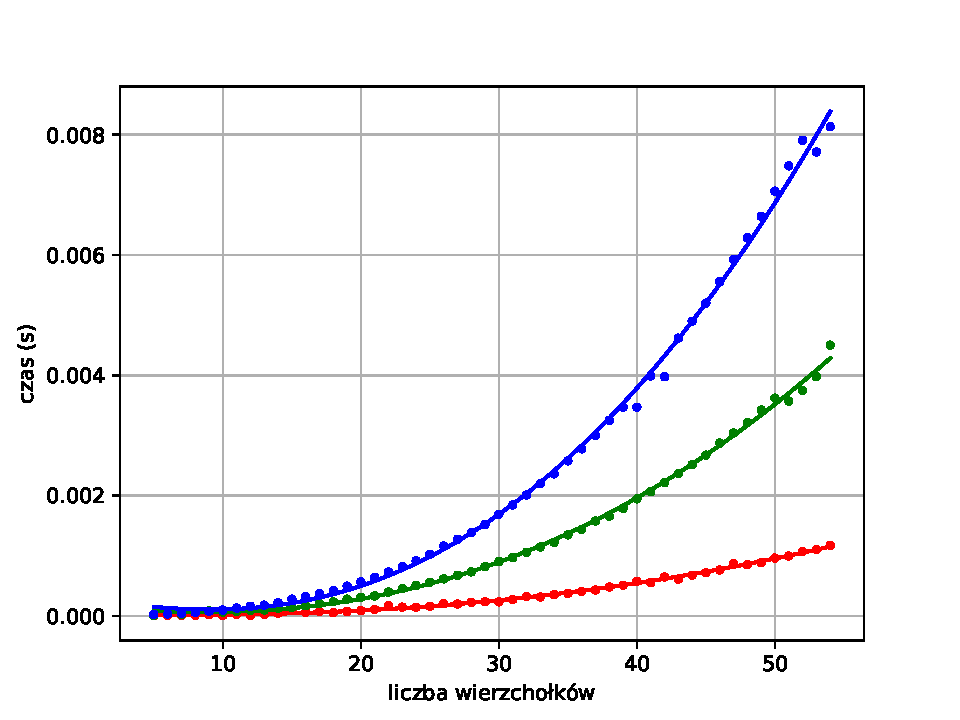
\includegraphics[width=0.9\textwidth]{images/Wykres_Dijkstra_gestosci.pdf}
\caption{Zależność czasu działania algorytmu Dijkstry od liczby wierzchołków w grafie i stałej gęstości (czerwone punkty - gęstość $0.1$, zielone punkty - gęstość $0.4$, niebieskie punkty - gęstość $0.8$). Linie ciągłe oznaczają aproksymacje odpowiednich wykresów punktowych.}
\label{rys_wykres_dij_gestosci}
\end{figure}

\begin{figure}[H]
\centering
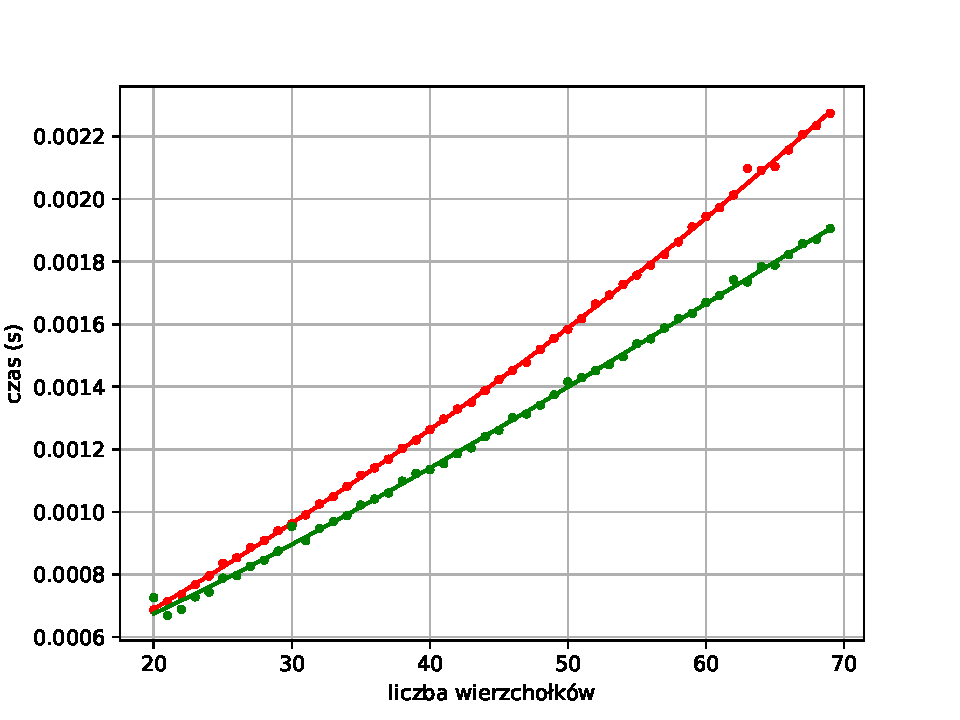
\includegraphics[width=0.9\textwidth]{images/Wykres_Dijkstra_naiwny_kolejka.pdf}
\caption{Porównanie czasu działania dwóch implementacji algorytmu Dijkstry w zależności od zmiany liczby wierzchołków przy stałej liczbie krawędzi. Punkty czerwone - implementacja z użyciem kolejki zaimplementowanej jako zwykła lista, punkty zielone - implementacja z użyciem kolejki zaimplementowanej z~użyciem kopców binarnych. Linie ciągłe -  aproksymacje odpowiednich wykresów punktowych.}
\label{rys_wykres_dij_naive}
\end{figure}



\subsubsection*{Algorytm Bellmana-Forda}
Podczas działania algorytmu Bellmana-Forda dokonywana jest $\big(|V| - 1\big)$-krotna relaksacja każdej krawędzi. Ponieważ graf zawiera $|E|$ krawędzi i dodatkowo wykonywane jest sprawdzanie wystąpienia cykli ujemnych ($|E|$-krotna iteracja), więc czas działania algorytmu wynosi $O(VE+E)= O(VE)$. Jeżeli mamy do czynienia z grafami gęstymi $|E|=O(V^2)$ to złożoność algorytmu Bellmana-Forda wynosi $O(V^3)$, a~w przypadku grafów rzadkich  $|E|=O(V)$ mamy do czynienia ze złożonością równą $O(V^2)$.

Na rysunku \ref{rys_wykres_b_f_gestosci} został pokazany wykres zależności czasu wykonania algorytmu Bellmana-Forda (implementacja przestawiona w rozdziale \ref{ch_3}) w zależności od liczby wierzchołków i stałej gęstości. Zostały użyte trzy zbiory grafów o gęstościach odpowiednio równych: $0.1$, $0.4$ i $0.8$. Zależności czasu działania algorytmu od zmiany liczby wierzchołków i krawędzi (różne gęstości) są zgodne z teoretycznym oszacowaniem. Porównując szybko wykresy z rysunków \ref{rys_wykres_dij_gestosci} i \ref{rys_wykres_b_f_gestosci} widzimy, że algorytm Bellmana-Forda jest ok. dziesięciokrotnie wolniejszy od algorytmu Dijkstry. Jest to oczywiście cena tego, że w przypadku algorytmu Bellmana-Forda możemy badać grafy o~wagach ujemnych, jak również wykrywać cykle ujemne.

\begin{figure}[H]
\centering
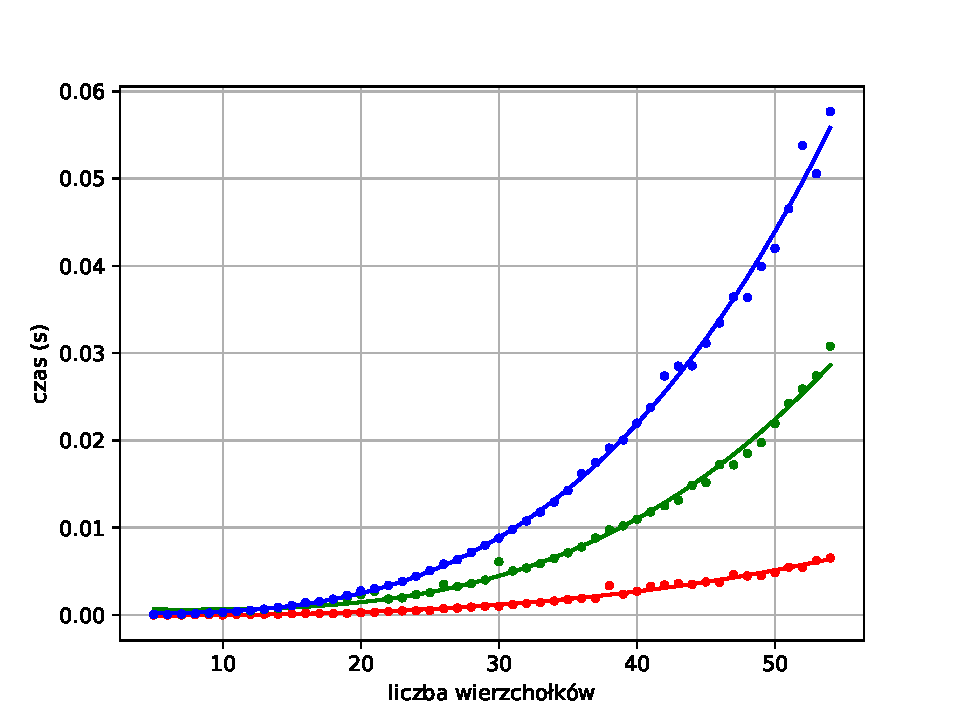
\includegraphics[width=0.9\textwidth]{images/Wykres_Bellman_Ford_gestosci.pdf}
\caption{Zależność czasu wykonywania algorytmu Bellmana-Forda od  liczby wierzchołków przy stałej gęstości (punkty czerwone - gęstość $0.1$, punkty zielone - gęstość $0.4$, punkty niebieskie - gęstość $0.8$).}
\label{rys_wykres_b_f_gestosci}
\end{figure}

\subsubsection*{Algorytm Dijkstry i Bellmana-Forda w kontekście problemu najkrótszych ścieżek między wszystkimi parami wierzchołków}
Jasne jest, że problem  najkrótszych ścieżek między wszystkimi parami wierzchołków może być rozwiązany, jeżeli wykonamy $|V|$ razy algorytm dla problemu najkrótszych ścieżek z jednym wierzchołkiem źródłowym. Jeżeli badamy graf ważony o wagach nieujemnych możemy zastosować algorytm  Dijkstry. Jeżeli implementacja kolejki priorytetowej będzie oparta o jednowymiarową tablicę z wyszukiwaniem liniowym, to czas działania takiego algorytmu będzie wynosił $O(V^3 + VE) = O(V^3)$. Natomiast, jeżeli do implementacji kolejki użyjemy kopców binarnych to złożoność algorytmu będzie równa $O(VE\log V)$, a w przypadku użycia kopów Fibonaciego mamy czas działania równy $O(V^2\log V+VE)$.

Z algorytmu Dijkstry nie możemy skorzystać, jeżeli w grafie dopuszczamy wagi o wartościach ujemnych. W takim przypadku możemy wykorzystać wolniejszy algorytm Bellmana-Forda używając go po razie dla każdego wierzchołka grafu. Czas działania tak otrzymanego algorytmu wynosi $O(V^2E)$, co dla grafów gęstych \big($|E|=O(V^2)$\big) daje $O(V^4)$.

\subsection{Najkrótsze ścieżki między wszystkimi parami wierzchołków}
Przejdziemy teraz do omówienia czasu działania trzech algorytmów służących do rozwiązywania problemu wyznaczania najkrótszych ścieżek między wszystkimi parami wierzchołków w grafach ważonych.

\subsubsection*{Algorytm z iloczynem odległości}

W rozdziale \ref{ch_3}  wykazaliśmy, że algorytm z iloczynem odległości  możemy w~łatwy sposób sprowadzić do problemu mnożenia macierzy. Stąd, czas działania tego algorytmy wynosi $O(V^4)$ - pojedyncze wykonanie mnożenia (iloczynu odległości) macierzy ma złożoność $O(V^3)$, ponadto algorytm oblicza ciąg $(V-1)$ macierzy. W ulepszonej wersji algorytmu liczba obliczanych iloczynów jest zredukowana do $\log(V-1)$, co daje łączny czas działania algorytmu równy $O(V^3 \log V)$. 

\begin{figure}[H]
\centering
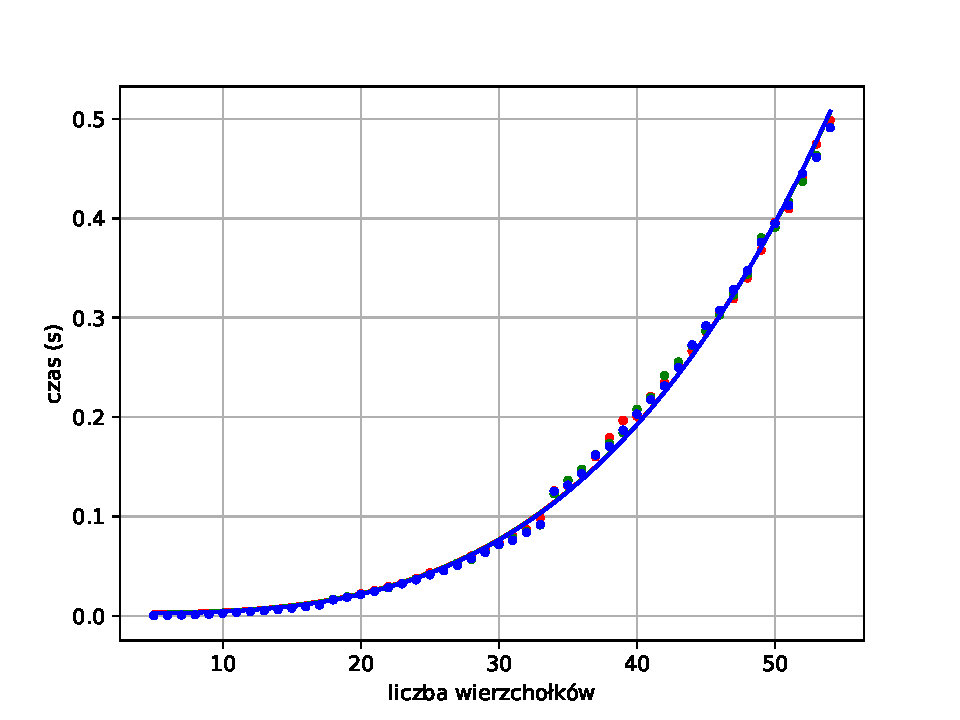
\includegraphics[width=0.75\textwidth]{images/Wykres_Macierze_gestosci.pdf}
\caption{Zależność czasu wykonywania algorytmu z iloczynem odległości od liczby wierzchołków grafu przy stałej gęstości (kolor czerwony - gęstość $0.1$, kolor zielony - gęstość $0.4$, kolor niebieski - gęstość $0.8$).}
\label{rys_wykres_matrix_gestosci}
\end{figure}

Rysunek \ref{rys_wykres_matrix_gestosci} przedstawia wykres, na którym widzimy zależność czasu wykonania ulepszonej wersji algorytmu z iloczynem odległości zaimplementowanego w rozdziale \ref{ch_3} od liczby wierzchołków dla grafów o stałej gęstości. Tak jak we wcześniejszych analizach zostały użyte trzy zbiory grafów o gęstościach odpowiednio $0.1$, $0.4$ i $0.8$. Złożoność czasowa tego algorytmu, jak i algorytmu Floyda-Warshalla nie jest zależna od liczby krawędzi (obydwa algorytmy wykorzystują reprezentację macierzową grafu), a co za tym idzie zmiana gęstości przy ustalonej liczbie wierzchołków nie ma wpływu na czas działania - widzimy, że wykresy dla wspominanych gęstości pokrywają się.




\subsubsection*{Algorytm Floyda-Warshalla}
Złożoność czasowa algorytmu Floyda-Warshalla jest bardzo prosta do wyznaczenia. Wykonywanych jest $|V|$ iteracji dla macierzy o wymiarach $|V|\times |V|$ co daje złożoność $O(V^3)$.

\begin{figure}[H]
	\centering
	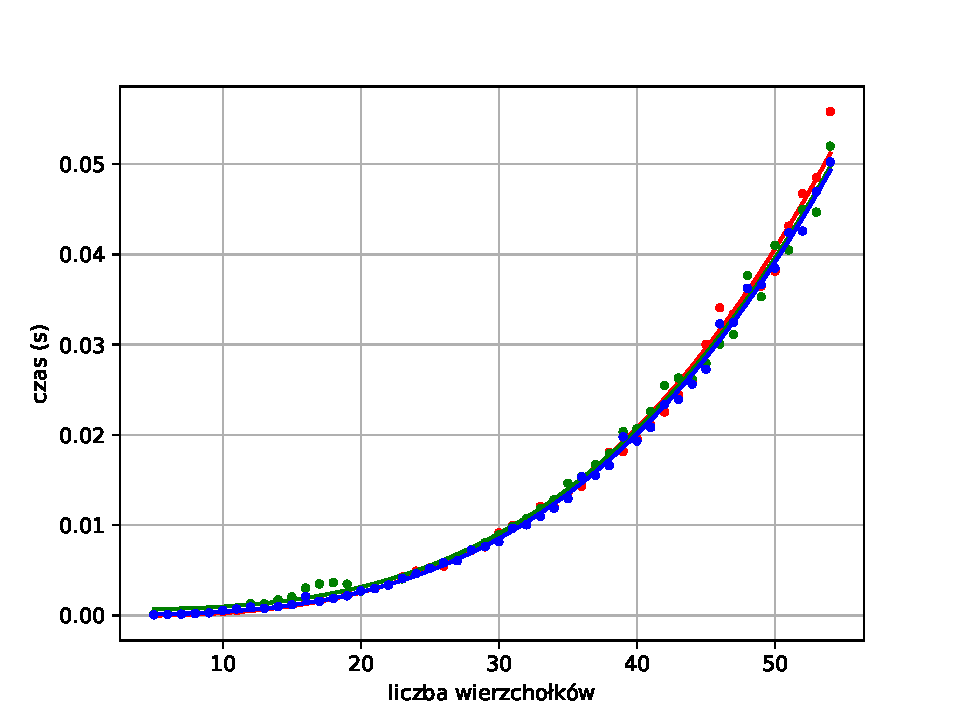
\includegraphics[width=0.75\textwidth]{images/Wykres_Floyd_Warshall_gestosci.pdf}
\caption{Zależność czasu wykonywania algorytmu Floyda-Warshalla od liczby wierzchołków grafu przy stałej gęstości (kolor czerwony - gęstość $0.1$, kolor zielony - gęstość $0.4$, kolor niebieski - gęstość $0.8$).}
	\label{rys_wykres_f_w_gestosci}
	\end{figure}

Na rysunku \ref{rys_wykres_f_w_gestosci} został pokazany wykres zależności czasu wykonania algorytmu Floyda-Warshalla zaimplementowanego w rozdziale \ref{ch_3} od liczby wierzchołków dla grafów o stałej gęstości. Podobnie jak poprzednio zostały użyte trzy zbiory grafów o gęstościach $0.1$, $0.4$ i $0.8$. Jak już wypominaliśmy przy okazji analizy algorytmu z iloczynem odległości, wykres ukazuje brak zależności czasu działania algorytmu Floyda-Warshall od liczby krawędzi grafu. Porównując wykresy na rysunkach \ref{rys_wykres_matrix_gestosci} i~\ref{rys_wykres_f_w_gestosci} widzimy, że zgodnie z oczekiwaniami algorytm Floyda-Warshalla jest znacznie szybszy niż algorytm z iloczynem odległości.



\subsubsection*{Algorytm Johnsona}

W algorytmie Johnsona budowa nowego grafu za pomocą algorytmu Bellmana-Forda wykonywane jest w czasie $O(VE)$. Dla tak zbudowanego grafu używamy algorytmu Dijkstry więc złożoność jest zależna od implementacji algorytmu Dijkstry. W przypadku implementacji używającej kolejki priorytetowej opartej na kopcach binarnych złożoność wyniesie $O(VE \log V + VE)$, używając bardziej skomplikowanej implementacji kolejki opartej na kopcach Fibonacciego uzyskamy złożoność $O(V^2 \log V + VE)$. Jak łatwo zauważyć algorytm Johnsona ma niższą złożoność dla grafów rzadkich niż algorytm Floyda-Warshalla. W przypadku grafów gęstych algorytm Floyda-Warshalla o złożoności $O(V^3)$ jest o wiele bardziej wydajny. 

\begin{figure}[H]
\centering
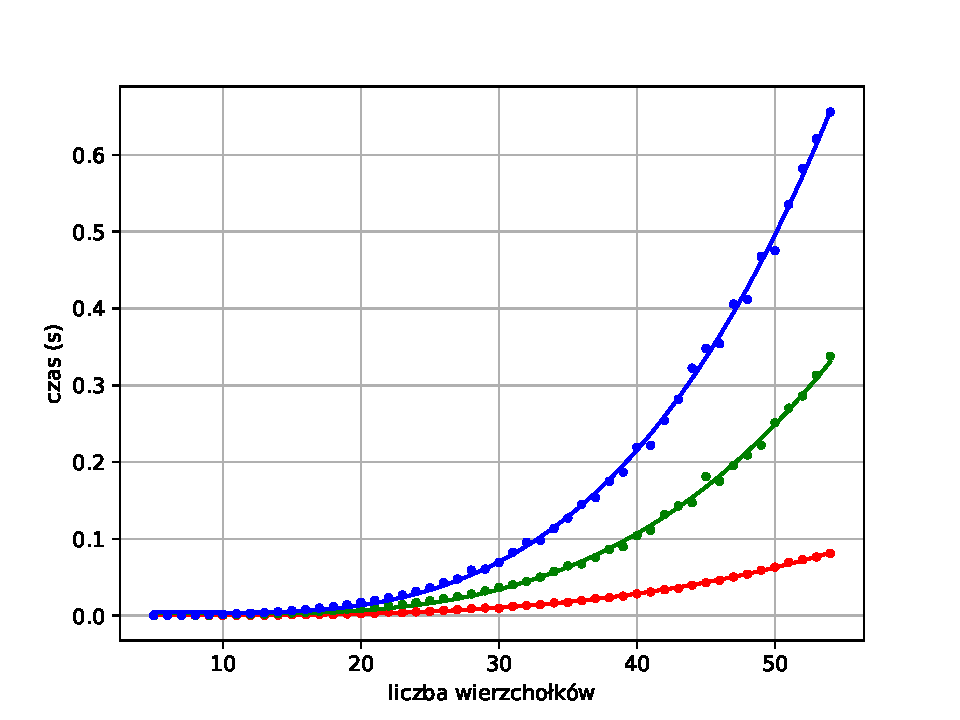
\includegraphics[width=0.75\textwidth]{images/Wykres_Johnson_gestosci.pdf}
\caption{Wykres zależności czasu działania algorytmu Johnsona od liczby wierzchołków przy stałej gęstości. (punkty czerwone - gęstość $0.1$, punkty zielone - gęstość $0.4$, punkty niebieskie - gęstość $0.8$)}
\label{rys_wykres_johnson_gestosci}
\end{figure}

Na rysunku \ref{rys_wykres_johnson_gestosci} został pokazany wykres zależności czasu wykonania algorytmu Johnsona zaimplementowanego w rozdziale \ref{ch_3} od liczby wierzchołków dla grafów o~stałej gęstości. Tu również zostały użyte trzy zbiory grafów o gęstościach $0.1$, $0.4$ i $0.8$. Z wykresu możemy zauważyć, że czas wykonania algorytmu Johnsona szybko rośnie dla dużych ilości wierzchołków i dużych gęstości grafów. Jeśli porównamy wykres dla algorytmu Floyda-Warshalla i wykres dla algorytmu Johnsona można stwierdzić, że na ogół algorytm Floyda-Warshalla jest znacznie szybszy jednak dla grafów wystarczająco rzadkich, algorytm Johnsona działa efektywniej - wrócimy do tego problem w dalszej części tego rozdziału.



\section{Dalsze porównania czasów działania algorytmów}

W tej sekcji skupimy się na dodatkowej analizie czasu działania algorytmów zaimplementowanych w rozdziale \ref{ch_3} w celu sprawdzenia czy złożoność czasowa tych algorytmów jest zgodna z założeniami. 
Podczas omawiania złożoności czasowej algorytmów analizowaliśmy już czas działania naszych implementacji dla zmiennej liczby wierzchołków, ale przy zachowaniu stałej gęstości grafu.

\subsection*{Porównanie dla stałej liczby wierzchołków}

Porównamy teraz między sobą czasy działania wybranych algorytmów dla grafów o stałej liczbie wierzchołków, lecz zmieniającej się liczbie krawędzi. Liczba wierzchołków będzie stała i równa $50$, liczba krawędzi będzie rosła od $0$ do maksymalnej ilości krawędzi w grafie z $50$ wierzchołkami tj. wartości równej $2450$ z krokiem równym $50$.

\begin{figure}[H]
\centering
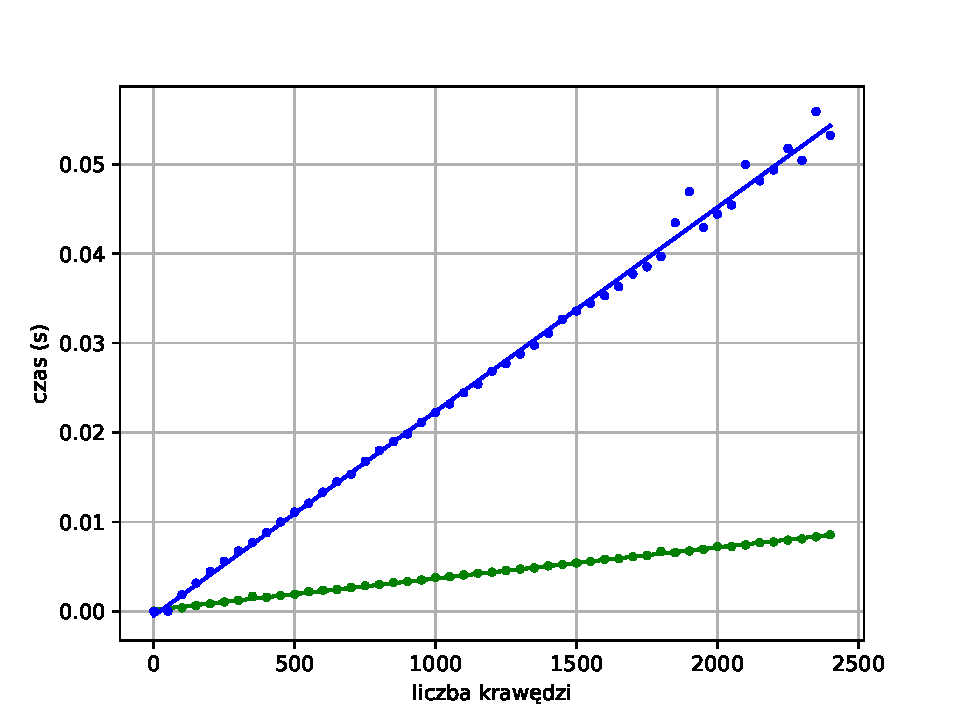
\includegraphics[width=0.75\textwidth]{images/Wykres_stale_wierzcholki_Dijkstra_Bellman_Ford.pdf}
\caption{Zależność czasu działania algorytmów Dijkstry i Bellmana-Forda od liczby krawędzi przy stałej liczbie wierzchołków (zielone punkty - algorytm Dijkstry, niebieski punkty - algorytm Bellmana-Forda). Linie ciągłe oznaczają aproksymacje odpowiednich wykresów punktowych.}
\label{rys_wykres_wierzch_dij_b_f}
\end{figure}

\begin{figure}[H]
\centering
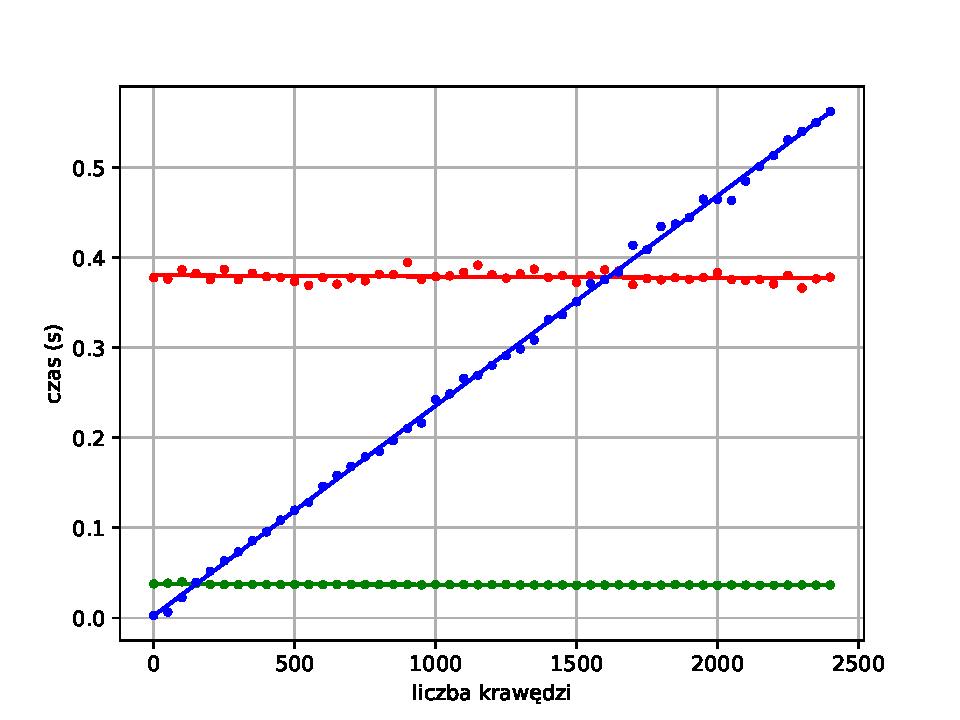
\includegraphics[width=0.75\textwidth]{images/Wykres_stale_wierzcholki_Matrix_Floyd_Warshall_Johnson.pdf}
\caption{Zależność czasu działania algorytmów z iloczynem odległości, Floyda-Warshalla i Johnsona od liczby krawędzi przy stałej liczbie wierzchołków (czerwone punkty - algorytm z  iloczyn odległości, zielone punkty - algorytm Floyda-Warshalla, niebieskie punkty - algorytm Johnsona). Linie ciągłe oznaczają aproksymacje odpowiednich wykresów punktowych.}
\label{rys_wykres_wierzch_mm_fw_j}
\end{figure}

Porównanie algorytmu Dijkstry i Bellmana-Forda (rysunek \ref{rys_wykres_wierzch_dij_b_f}) jest jednoznaczne. Algorytm Dijkstry jest stanowczo szybszy niż Bellmana-Forda. Porównanie algorytmów z iloczynem odległości, Floyda-Warshalla oraz algorytmu Johnsona (rysunek \ref{rys_wykres_wierzch_mm_fw_j}) również potwierdza teoretyczne założenia, algorytm Johnsona dla małej ilości krawędzi (czyli dla grafów rzadkich) będzie szybszy, lecz muszą to być naprawdę rzadkie grafy; po przekroczeniu pewnej ilości krawędzi czas wykonywania algorytmu Johnsona rośnie liniowo w przeciwieństwie do algorytmów z iloczynem odległości i~Floyda-Warshalla, które nie są zależne od ilości krawędzi.



\subsection*{Porównanie dla stałej liczby krawędzi}

Dokonamy teraz porównania między sobą czasów działania wybranych algorytmów dla grafów o stałej liczbie krawędzi, lecz zmieniającej się liczbie wierzchołków. W tym przypadku ilość wierzchołków będzie rosła od $20$ do $70$, ilość krawędzi będzie stała i równa $380$ (maksymalna liczba krawędzi dla grafu o $20$ wierzchołkach). Oczywiście w tym przypadku gęstość grafu będzie się  stale zmniejszać.

Zgodnie z oczekiwaniami algorytm Dijkstry w tym przypadku również jest lepszy niż algorytm Bellmana-Forda (rysunek \ref{rys_wykres_kraw_dij_b_f}).

\begin{figure}[H]
\centering
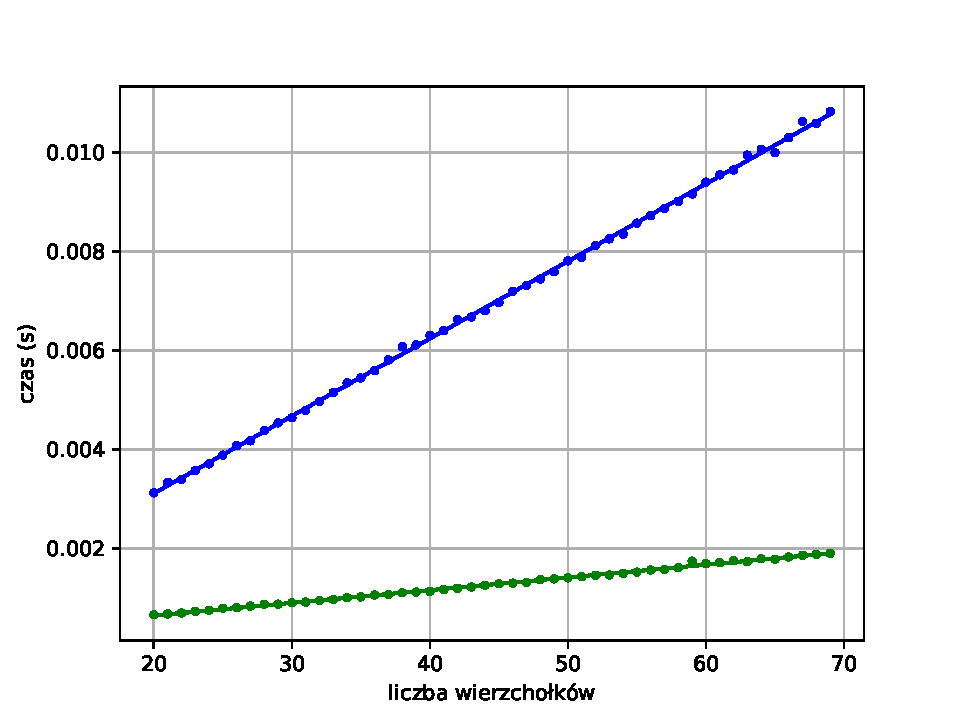
\includegraphics[width=0.75\textwidth]{images/Wykres_stale_krawedzie_Dijkstra_Bellman_Ford.pdf}
\caption{Zależność czasu działania algorytmów Dijkstry i~Bellmana-Forda od liczby wierzchołków przy ustalonej liczbie krawędzi (kolor zielony - algorytm Dijkstry, kolor niebieski - algorytm Bellmana-Forda).}
\label{rys_wykres_kraw_dij_b_f}
\end{figure}

\begin{figure}[H]
\centering
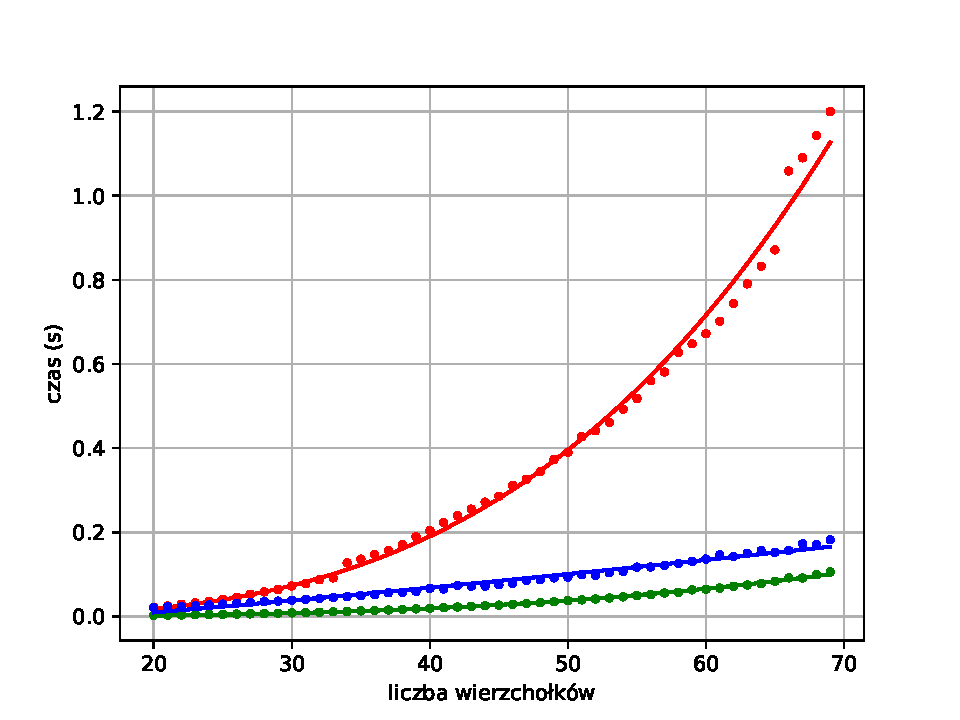
\includegraphics[width=0.75\textwidth]{images/Wykres_stale_krawedzie_Matrix_Floyd_Warshall_Johnson.pdf}
\caption{Zależność czasu działania algorytmów z iloczynem odległości, Floyda-Warshalla i Johnsona od liczby wierzchołków przy stałej liczbie krawędzi w grafie (czerwone punkty - algorytm z iloczynem odległości, zielone punkty - algorytm Floyda-Warshalla, niebieskie punkty - algorytm Johnsona).  Linie ciągłe oznaczają aproksymacje odpowiednich wykresów punktowych.}
\label{rys_wykres_kraw_mm_fw_j}
\end{figure}

Podobnie porównanie algorytmów z iloczynem odległości, Floyda-Warshalla oraz Johnsona pokazuje, że wraz ze wzrostem liczby wierzchołków czas wykonywania znacznie wzrasta zgodnie z teoretycznymi oczekiwaniami. Spośród tych trzech algorytmów najwolniejszy jest algorytm z iloczynem odległości. Wzrost czasu działania algorytmu Johnsona i Floyda-Warshalla jest podobny, lecz to ten drugi przeważnie jest szybszy. W celu lepszego porównania tych dwóch algorytmów użyjemy osobnego wykresu (rysunek \ref{rys_wykres_kraw_fw_j}). Widać, że w przypadku stałej ilości krawędzi czas działania algorytmu Floyda-Warshalla jest lepszy, ale rośnie z podobną szybkością jak czas działania algorytmu Johnsona. 

\begin{figure}[H]
\centering
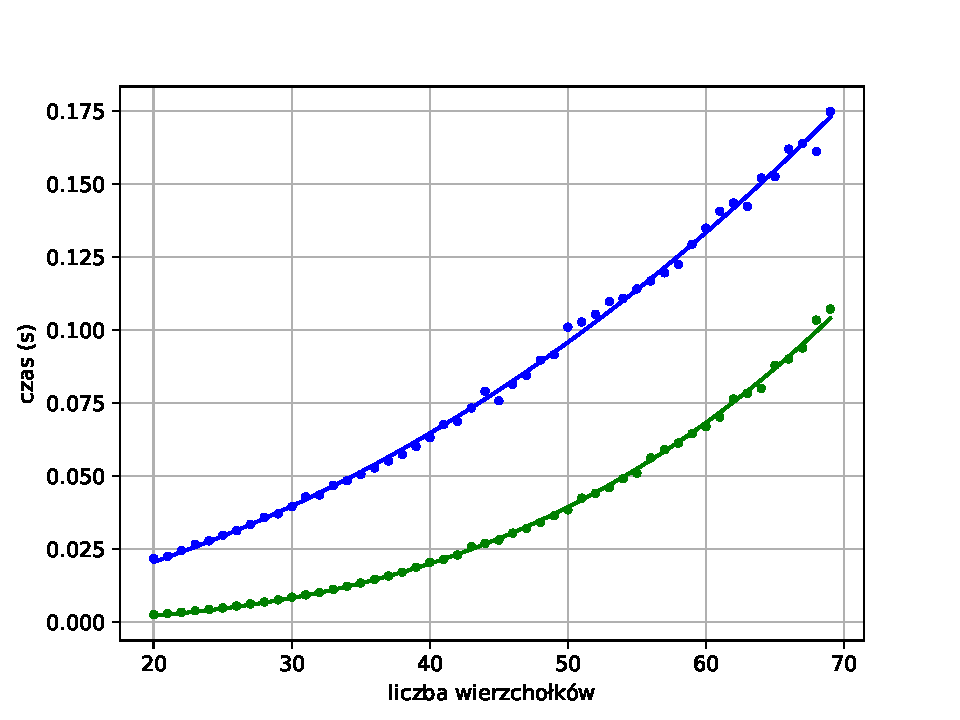
\includegraphics[width=0.75\textwidth]{images/Wykres_stale_krawedzie_Floyd_Warshall_Johnson.pdf}
\caption{Porównanie czasu działania algorytmów Floyda-Warshalla i Johnsona w zależności od liczby wierzchołków przy ustalonej liczbie krawędzi (zielone punkty - Floyda-Warshalla, niebieskie punkty - algorytm Johnsona).  Linie ciągłe oznaczają aproksymacje odpowiednich wykresów punktowych.}
\label{rys_wykres_kraw_fw_j}
\end{figure}

\subsection*{Algorytm Dijkstry dla ścieżek między wszystkim parami wierzchołków}

Przedstawimy teraz porównanie algorytmu Dijkstry w przypadku zastosowania go do wyznaczania najkrótszych ścieżek między wszystkimi parami wierzchołków z~algorytmem Floyda-Warshalla oraz algorytmem Johnsona. W tym celu wykorzystamy  grafy o stałej gęstości równej $0.4$. Oczywiście należy uwzględnić fakt, że ponieważ używamy algorytmu Dijkstry to rozważamy grafy o nieujemnych wagach.

Rysunek \ref{rys_wykres_dijkstra_all_johnson} pokazuje porównanie czasów działania wspomnianych algorytmów. Analizując ten wykres mogłoby się wydawać, że tak użyty algorytm Dijsktry nie jest znacząco lepszy niż algorytm Johnsona. Pamiętajmy jednak, że algorytm Johnsona wykorzystuje algorytm Dijsktry właśnie w takiej postaci, a badamy tu czas działania tylko pod względem zmiany liczby wierzchołków. Ponadto po raz kolejny widać, że algorytm Floyda-Warshalla jest praktycznie zawsze najlepszym wyborem w przypadku problemu najkrótszych ścieżek miedzy wszystkimi parami wierzchołków. 

\begin{figure}[H]
\centering
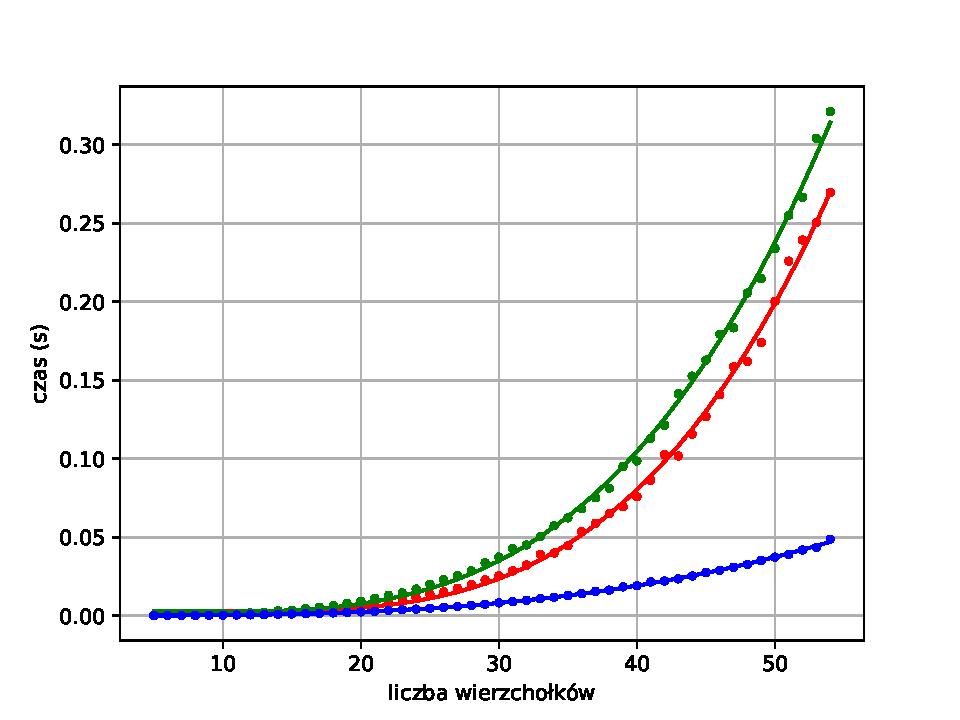
\includegraphics[width=0.9\textwidth]{images/Wykres_Dijkstra_all_vs_Johnson.pdf}
\caption{Zależność czasu działania algorytmów Johnsona, Dijkstry dla wszystkich wierzchołków oraz Floyda-Warshalla od liczby wierzchołków przy stałej gęstości grafu (czerwone punkty - algorytm Dijkstry dla wszystkich wierzchołków, zielone punkty - algorytm Johnsona, niebieskie punkty - algorytm Floyd-Warshall).}
\label{rys_wykres_dijkstra_all_johnson}
\end{figure}

\subsection*{Algorytm Johnsona a pojęcie grafu gęstego}

Wspominaliśmy już w tym rozdziale, że algorytm Johnsona jest szybszy niż Floyda-Warshalla dla grafów rzadkich. Problemem jest jednak fakt, że nie ma ścisłej definicji kiedy dany graf możemy uznać za gęsty lub rzadki. W niniejszej sekcji przeprowadzimy krótką analizę, aby spróbować określić wartość graniczną gęstości dla której powiemy, że graf jest już gęsty.  W tym celu będziemy badać czasy działania algorytmu Johnsona i Floyda-Warshalla.


\begin{figure}[H]
\centering
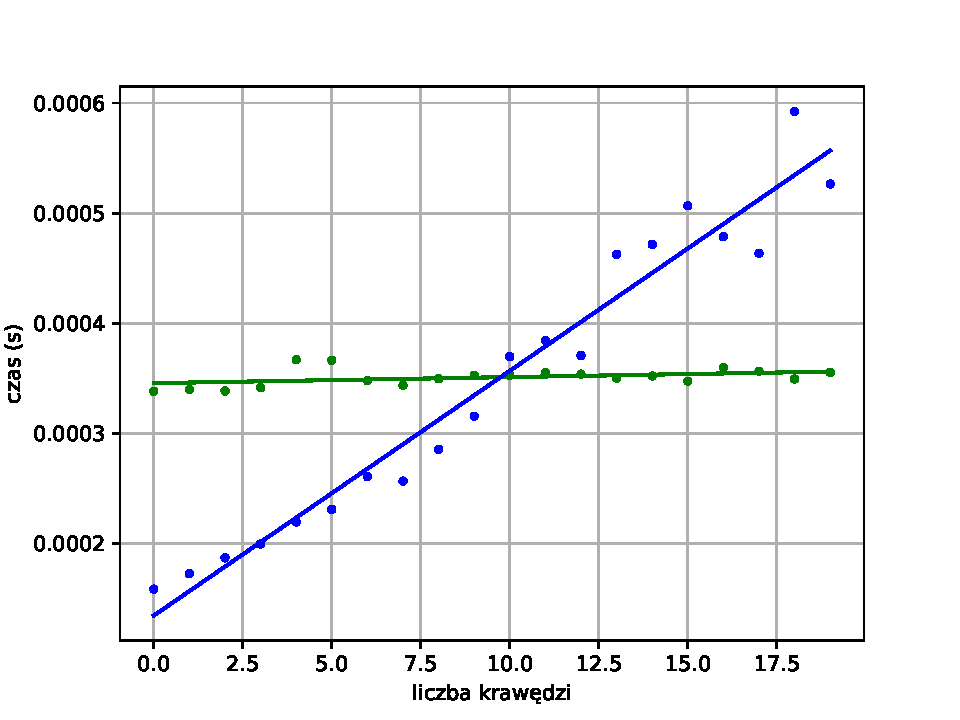
\includegraphics[width=0.8\textwidth]{images/Wykres_granica_gestego_grafu_10_wierzcholkow.pdf}
\caption{Zależność czasu działania algorytmów Johnsona i Floyda-Warshalla od liczby krawędzi przy stałej liczbie wierzchołków grafu równej $10$ (kolor zielony - algorytm Floyda-Warshalla, kolor niebieski - algorytm Johnson).}
\label{rys_wykres_gran_gest_10}
\end{figure}

\begin{figure}[H]
\centering
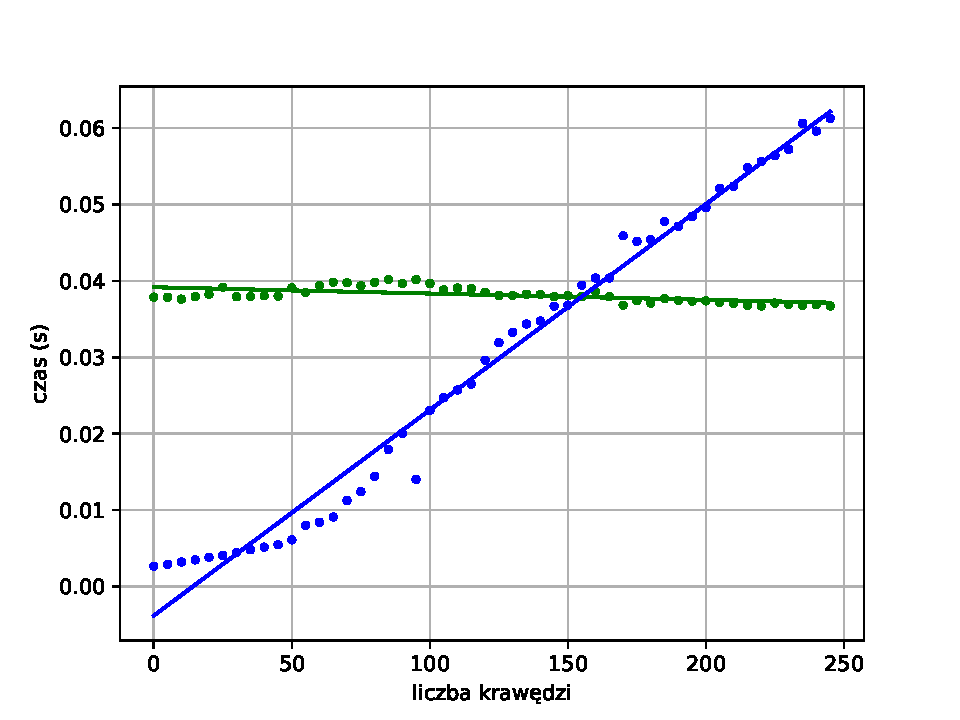
\includegraphics[width=0.8\textwidth]{images/Wykres_granica_gestego_grafu_50_wierzcholkow.pdf}
\caption{Zależność czasu działania algorytmów Johnsona i Floyda-Warshalla od liczby krawędzi przy stałej liczbie wierzchołków grafu równej $50$ (kolor zielony - algorytm Floyda-Warshalla, kolor niebieski - algorytm Johnsona).}
\label{rys_wykres_gran_gest_50}
\end{figure}

Zacznijmy od przypadku grafu mającego $10$ wierzchołków, w którym będziemy zwiększać liczbę krawędzi od $0$ do $20$. Stosowne porównanie czasów działania algorytmów przedstawia rysunek \ref{rys_wykres_gran_gest_10}. Możemy w przybliżeniu stwierdzić, że dla grafów, które mają powyżej dziewięciu krawędzi algorytm Floyda-Warshalla jest już szybszy. Dla grafu o $10$ wierzchołkach jest to gęstość w przybliżeniu równa  $0.1$, czyli bardzo mała. 

Następny analizowany przypadek to grafy ze stałą liczbą wierzchołków równą $50$ oraz liczbą krawędzi zmieniającą się od $0$ do $250$ z krokiem co $5$. Porównanie czasu działania obu algorytmów przedstawia wykres na rysunku \ref{rys_wykres_gran_gest_50}. Teraz, algorytm Johnsona staje się wolniejszy dla liczby krawędzi powyżej wartości ok. $150$ krawędzi, co daje gęstość równą $0.06$.

Kolejny przypadek to grafy o liczbie wierzchołków równej $100$ i liczbie krawędzi zmieniających się od $0$ do $1000$ z krokiem co $20$. Stosowane porównanie czasu działania algorytmów przedstawia rysunek \ref{rys_wykres_gran_gest_100}. Z wykresu można odczytać, że dla liczby krawędzi większej niż $400$ algorytm Floyda-Warshalla działa szybciej, co daje gęstość grafu równą ok. $0.04$. Możemy już przypuszczać, że nasza szukana wartość gęstości nie jest stała i maleje.

\begin{figure}[!htp]
\centering
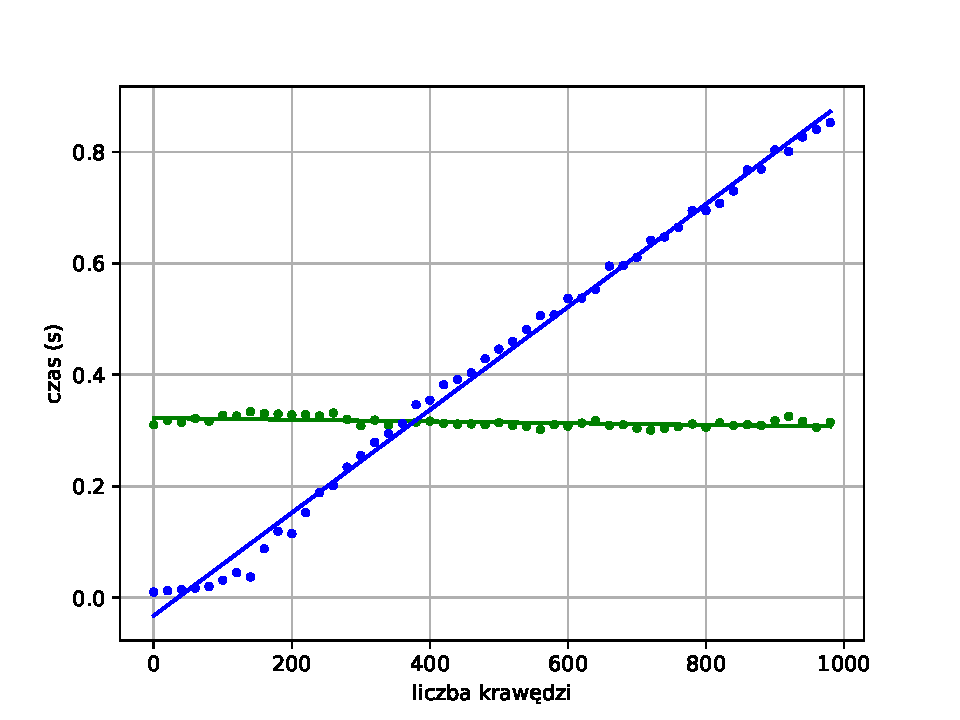
\includegraphics[width=0.8\textwidth]{images/Wykres_granica_gestego_grafu_100_wierzcholkow.pdf}
\caption{Zależność czasu działania algorytmów Johnsona i Floyda-Warshalla od liczby krawędzi przy stałej liczbie wierzchołków grafu równej $100$ (kolor zielony - algorytm Floyda-Warshalla, kolor niebieski - algorytm Johnsona).}
\label{rys_wykres_gran_gest_100}
\end{figure}

Ostatni przypadek, który rozważymy to grafy o stałej liczbie wierzchołków równej $150$ i zmieniającej się liczbie krawędzi od $0$ do $22350$ z krokiem co $45$. Porównanie czasu działania obu algorytmów dla takich grafów przedstawia wykres na rysunku \ref{rys_wykres_gran_gest_150}. Teraz, algorytm Johnsona staje się wolniejszy dla liczby krawędzi powyżej wartości ok. $600$, co daje gęstość równą $0.02$. Wynik ten potwierdza poprzednie przypuszczenia.

\begin{figure}[H]
\centering
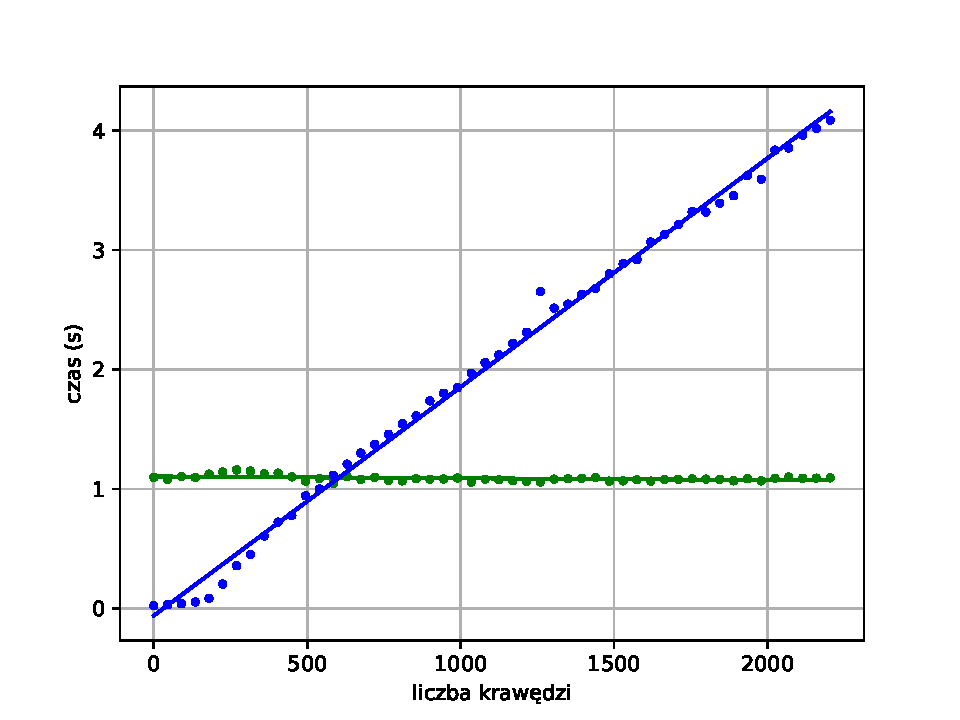
\includegraphics[width=0.8\textwidth]{images/Wykres_granica_gestego_grafu_150_wierzcholkow.pdf}
\caption{Zależność czasu działania algorytmów Johnsona i Floyda-Warshalla od liczby krawędzi przy stałej liczbie wierzchołków grafu równej $150$ (kolor zielony - algorytm Floyda-Warshalla, kolor niebieski - algorytm Johnsona).}
\label{rys_wykres_gran_gest_150}
\end{figure}

Na podstawie przeprowadzonej tej krótkiej analizy możemy stwierdzić, że mówienie o grafach rzadkich i gęstych chociażby tylko w kontekście algorytmu Johnsona jest dość niejednoznaczne i nie da się określić wartości granicznej gęstości dla której powiemy, że dany graf jest rzadki lub gęsty.

\section{Podsumowanie}

Do wyznaczania ścieżek z jednym wierzchołkiem źródłowym w grafie ważonym bez wag ujemnych najlepszym wyborem będzie algorytm Dijkstry. Jeżeli graf posiada ujemne wagi to musimy skorzystać z algorytmu Bellmana-Forda licząc się z~tym, że jest to algorytm wolniejszy. Ponadto, algorytm  Bellmana-Forda możemy wykorzystywać do wykrywania cykli ujemnych. W przypadku problemu wyznaczania najkrótszych ścieżek między wszystkimi parami wierzchołków grafu ważonego najlepszym wyborem będzie algorytm Floyda-Warshalla. Jedynie w przypadku grafów odpowiednio rzadkich warto rozważyć użycie algorytmu Johnsona.

\chapter*{Zakończenie}

\addcontentsline{toc}{chapter}{Zakończenie}
W niniejszej pracy zostały przedstawione podstawowe pojęcia teorii grafów oraz najważniejsze algorytmy wyznaczające najkrótsze ścieżki w grafach ważonych, które są  powszechnie wykorzystywane w praktyce. Można zauważyć podział pracy na część teoretyczną oraz praktyczną.

Cześć teoretyczna pracy, dokładniej są to rozdziały \ref{ch_1} i \ref{ch_2}, skupia się na podstawowych informacjach z teorii grafów oraz na dokładnym opisie wspomnianych algorytmów bazujących na wybranych  informacjach z literatury \cite{ALG_BEZ_TAJ,CORMEN, KOR&LYCZ, WOJ&PIEN}.

Cześć praktyczna, rozdziały \ref{ch_3} i \ref{ch_4}, skupia się na implementacji algorytmów w języku Python oraz analizie i porównaniu tych implementacji w celu niejako sprawdzania ich poprawności - badana była złożoność czasowa zaimplementowanych algorytmów.

Głównym osiągnięciem autora pracy jest przedstawienie w zwięzły sposób opisu teoretycznego omawianych algorytmów, a przede wszystkim samodzielna ich implementacja w~języku Python. Autor pracy przeprowadził także w rozdziale \ref{ch_4} analizę złożoności czasowej swoich implantacji, która to zgadza się z teoretycznymi założeniami. 

Na końcu pracy umieszczono dwa dodatki. Pierwszy z nich zawiera krótkie informacje na temat złożoności obliczeniowej i notacji asymptotycznej. Drugi zawiera wybrane kody źródłowe w języku Python wykorzystane w niniejszej pracy. Wszystkie kody źródłowe, które autor napisał na potrzeby niniejszej pracy zostały załączone na nośniku CD. Można je wykorzystać, by porównać wyniki na różnych maszynach obliczeniowych

Podsumowując, treść zawarta w niniejszej pracy pozwala w prosty i czytelny sposób zaznajomić się z tematyką grafów oraz algorytmów wyznaczających najkrótsze ścieżki w grafach ważonych i może zostać użyta jako podstawowe źródło wiedzy na ich temat. 


\appendix
%######################################################################################
%@@@@@@@@@@@@@@@@@@@@@@@@@@@@@@@@@@@@@@@@@@@@@@@@@@@@@@@@@@@@@@@@@@@@@@@@@@@@@@@@@@@@@@
%######################################################################################

\chapter*{Dodatki}

\addcontentsline{toc}{chapter}{\numberline{6}Dodatki}

%\chapter{Dodatki}
%\appendix
\renewcommand{\thesection}{\Alph{section}}
\renewcommand\thefigure{\thesection.\arabic{figure}}    
\setcounter{figure}{0} 

%\addcontentsline{toc}{chapter}{Dodatki}
%\appendix
%\renewcommand{\thesection}{\Alph{section}}
%\renewcommand{\theequation}{\Alph{section}.\arabic{equation}}
%\renewcommand{\thefigure}{\Alph{section}.\arabic{figure}}


%--------------------------------------------------------------------------------------
%######################################################################################
%--------------------------------------------------------------------------------------

\section{Elementy złożoności obliczeniowej i notacja asymptotyczna}\label{dodatek:zlo}

\numberwithin{de}{section}
W niniejszym dodatku podamy pewne definicje istotne z punktu widzenia analizy algorytmów. Te informacje jak i ich uzupełnienie można znaleźć między innymi w~pracach~ \cite{CORMEN, KOT, WOJ&PIEN}.
\begin{de}
\textit{Złożonością obliczeniową} algorytmów nazywamy miarę, która określa ilość zasobów niezbędnych do wykonania danego algorytmu. Mówiąc o zasobach zwykle mamy na myśli czas i mówimy wtedy o \textit{złożoności czasowej} lub zajętość pamięci i w takim przypadku mamy do czynienia ze \textit{złożonością pamięciową}.
\end{de}

Większość zagadnień obliczeniowych ma wspólną cechę – im większe są rozmiary danych wejściowych, tym więcej zasobów (czasu, pamięci) jest koniecznych do wykonania danych obliczeń. Możemy zatem śmiało powiedzieć, że złożoność algorytmu jest funkcją rozmiaru danych wejściowych.

Przeważnie podczas analizy algorytmów to jego czas działania odgrywa większe znaczenie. Czas działania algorytmu zależy nie tylko od niego samego ale też od szybkości działania komputera, rodzaju danych i ich wielkości. Ponadto, program napisany w języku maszynowym będzie działał szybciej niż  ten napisany w~języku interpretowanym przez system operacyjny.  Dlatego, w celu uzależnienia się od konkretnego komputera zamiast zamiast czasu określa się ilości wykonywanych operacji elementarnych (podstawowych) o których zakładamy, że wykonują się w jednakowym czasie. Inaczej mówiąc miarą złożoności czasowej jest liczba operacji podstawowych w zależności od rozmiaru wejścia. Za operacje elementarne przyjmuje się np.: operacje arytmetyczne, logiczne i relacyjne; postawienie; indeksowanie lub odwołanie do pola struktury; przekazywanie wartości do funkcji; inicjalizacja wywołania funkcji.
\begin{de}
\textit{Złożonością pesymistyczną} nazywamy złożoność algorytmu, która jest wyznaczona w najgorszym przypadku. Dokładniej, jeżeli $D$ jest zbiorem wszystkich możliwych danych wejściowych, $d$ oznacza jeden z elementów zbioru $D$, a $f$ jest funkcją, która dla danego zestawu danych wejściowych $d$ zwraca liczbę operacji podstawowych to złożoność pesymistyczną możemy definiować następująco:
$$
\sup\{f(d)\colon\;d\in D\}.
$$
\end{de}
\begin{de}
Niech $D$ będzie zbiorem wszystkich możliwych danych wejściowych algorytmu, $d$ oznacza pojedynczy zestaw danych wejściowych ze zbioru $D$, $f$ jest funkcją, która dla danego $d$ zwraca liczbę operacji podstawowych. 
\textit{Złożoność oczekiwana} (\textit{średnia}) określa złożoność średnią, czyli wartość oczekiwaną funkcji $f$ traktowanej jako zmienną losową. Jeżeli wszystkie dane wejściowe są jednakowo prawdopodobne (z prawdopodobieństwem różnym od zera), wtedy złożoność oczekiwaną możemy wyznaczyć według wzoru:
$$
\frac{\displaystyle\sum_{d\in D}f(d)}{|D|}
$$
\end{de}

Wyznaczenie dokładnej postaci funkcji danych wejściowych opisującej złożoność obliczeniową algorytmu przeważnie nie jest zadaniem prostym, ale w praktyce wystarczą jej oszacowania. Najbardziej powszechną miarą do zapisu szacowania złożoności jet \textit{$O$-notacja} dotycząca kresu górnego.

\begin{de}
Niech będą dane dwie funkcje $f$ i $g$ o wartościach nieujemnych: $f,g\colon\bN\to\bR^{+}$. Mówimy, że funkcja $f = f(n)$ jest co najwyżej rzędu $g = g(n)$, czyli ma złożoność $O(g(n))$, jeżeli:
$$
\exists_{c>0}\exists_{n_0>0}\forall_{n>n_0} f(n)\leq c\cdot g(n).
$$
Inaczej:
$$
f(n) = O(g(n))\equiv\limsup_{n\to\infty}\left|\frac{f(n)}{g(n)}\right|<\infty.
$$
\end{de}
Możemy powiedzieć nieformalnie, że funkcja $g$ jest kresem górnym dla funkcji $f$. Ponieważ dla danej funkcji $f$ może istnieć niekończenie wiele takich funkcji to w~praktyce  w celu uniknięcia niejednoznaczności wybiera się najmniejszą funkcję $g$~o tej własności.

Innymi miarami do do szacowania złożoności są \textit{$\Omega$-notacja} i \textit{$\Theta$-notacja}, jednak są one rzadziej stosowane.

\begin{de}
Niech będą dane dwie funkcje $f$ i $g$ o wartościach nieujemnych: $f,g\colon\bN\to\bR^{+}$. Mówimy, że funkcja $f = f(n)$ jest co najmniej rzędu $g = g(n)$, czyli ma złożoność $\Omega(g(n))$, jeżeli:
$$
\exists_{c>0}\exists_{n_0>0}\forall_{n>n_0} f(n)\geq c\cdot g(n).
$$
Inaczej:
$$
f(n) = \Omega(g(n))\equiv\liminf_{n\to\infty}\left|\frac{f(n)}{g(n)}\right|>0.
$$
\end{de}
Możemy powiedzieć nieformalnie, że funkcja $g$ jest kresem dolnym dla funkcji $f$. Ponieważ dla danej funkcji $f$ może istnieć niekończenie wiele takich funkcji to w~praktyce w celu uniknięcia niejednoznaczności wybiera się największą funkcję $g$~o~tej własności.

\begin{de}
Notacja $\Theta$ jest połączeniem notacji $O$ oraz $\Omega$. Niech będą dane dwie funkcje $f$ i $g$ o wartościach nieujemnych: $f,g\colon\bN\to\bR^{+}$. Mówimy, że funkcja $f = f(n)$ jest co najmniej rzędu $g = g(n)$, czyli ma złożoność $\Theta(g(n))$, jeżeli $f(n) = \Omega(g(n))$ oraz $f(n) = O(g(n))$
\end{de}
Można by pomyśleć, że notacja $\Theta$ jest najlepsza i najbardziej dokładna ale jest to mylne przekonanie i w praktyce notacja ta jest rzadko używana.

%--------------------------------------------------------------------------------------
%######################################################################################
%--------------------------------------------------------------------------------------

\section{Wybrane kody źródłowe}\label{dodatek:kody}

\lstinputlisting[label = Python_print_dijkstra, caption = {Kod \'{z}r\'{o}d\l{}owy funkcji pomocniczej wypisuj\k{a}cej wyniki algorytmu Dijkstry.}]{python_source/print_dijkstra.py}

\lstinputlisting[label = Python_print_b_f, caption = {Kod \'{z}r\'{o}d\l{}owy funkcji pomocniczej wypisuj\k{a}cej wyniki algorytmu Bellmana-Forda.}]{python_source/print_bellman_ford.py}

\lstinputlisting[label = Python_print_f_w, caption = {Kod \'{z}r\'{o}d\l{}owy funkcji pomocniczej wypisuj\k{a}cej wyniki algorytmu Floyda-Warshalla.}]{python_source/print_floyd_warshall.py}

\lstinputlisting[label = Python_print_johnson, caption = {Kod \'{z}r\'{o}d\l{}owy funkcji pomocniczej wypisuj\k{a}cej wyniki algorytmu Johnsona.}]{python_source/print_Johnson.py}

\lstinputlisting[label = Python_generator, caption = {Kod \'{z}r\'{o}d\l{}owy funkcji generuj\k{a}cej losowe grafy.}]{python_source/generator.py}

\lstinputlisting[label = Python_zapis_do_pliku, caption = {Kod \'{z}r\'{o}d\l{}owy przyk\l{}adowego zapisu wygenerowanych graf\'{o}w do pliku.}]{python_source/graph_to_file.py}

\lstinputlisting[label = Python_make_plot, caption = {Kod \'{z}r\'{o}d\l{}owy funkcji tworz\k{a}cej pojedynczy wykres dla jednej funkcji, na g\l{}\'{o}wnym wykresie (rysunku) mo\.ze by\'c wiele takich pojedynczych wykres\'{o}w.}]{python_source/make_plot.py}

\lstinputlisting[label = Python_make_plot_example, caption = {Kod \'{z}r\'{o}d\l{}owy pokazuj\k{a}cy u\.zycie funkcji \texttt{make}\_\texttt{plot}.}]{python_source/make_plot_example.py}

%--------------------------------------------------------------------------------------
%######################################################################################
%--------------------------------------------------------------------------------------

\def\bibname{Literatura}
\begin{thebibliography}{99}
\addcontentsline{toc}{chapter}{Literatura}

\bibitem{ALG_BEZ_TAJ}
T.H. Cormen, {\it Algorytmy bez tajemnic}, Wydawnictwo Helion, Gliwice, 2013.

\bibitem{CORMEN}
T.H. Cormen, C.E. Leiserson, R.L. Rivest, C.S. Stein, {\it Wprowadzenie do algorytmów}, Wydawnictwo Naukowe PWN, Warszawa, 2012.

\bibitem{KOR&LYCZ}
W. Kordecki, A. Łyczkowska-Hanćkowiak, {\it Matematyka dyskretna dla informatyków}, Wydawnictwo Helion, Gliwice, 2018.

\bibitem{KOT}
P. Kotowski, {\it Algorytmy + Struktury danych = Abstrakcyjne typy danych}, Wydawnictwo BTC, Warszawa 2006;

\bibitem{WOJ&PIEN}
K. Pieńkowski, J. Wojciechowski, {\it Grafy i sieci}, Wydawnictwo Naukowe PWN, Warszawa, 2013.

\bibitem{python_docs}
\url{https://docs.python.org/3/}

\bibitem{wiki_mosty}
\url{https://pl.wikipedia.org/wiki/Zagadnienie\_mostów\_królewieckich}

\end{thebibliography} 

\end{document}